


\begin{document}

\frontmatter % Use roman page numbering style (i, ii, iii, iv...) for the pre-content pages

\pagestyle{plain} % Default to the plain heading style until the thesis style is called for the body content

%----------------------------------------------------------------------------------------
%	TITLE PAGE
%----------------------------------------------------------------------------------------

% - - - - - - - début de la page
\thispagestyle{empty}

%
\includegraphics[scale=0.12]{upmc-logo.png}
\begin{titlepage}
        \begin{center}
            
\includegraphics[width=0.3\linewidth]{upmc-logo.png}
        \end{center}
       
        \begin{center}
           
            \textbf{TH\`ESE}\\
            présentée pour obtenir le grade de\\
            \vspace*{0.5cm}
            \begin{center}\textsc{Docteur de l'université Pierre et Marie Curie}\end{center} \ \\
           
            \vspace*{0.5cm}
           
            Sp\'ecialit\'e \textsc{Informatique}\ \\
           
            \vspace*{0.5cm}
           
            École doctorale Informatique, Télécommunications et Électronique (Paris)
            \vspace*{1cm}
           
        \end{center}
       
            % Thesis title
            {\color{briquered} \hrule height 2px }
            \vspace*{0.3cm}
            {\LARGE\centering \textsc{\ttitle\\ }}
            \vspace*{0.5cm}
            {\color{briquered} \hrule height 2px }
            \vspace*{1cm}
            \begin{center}
            {\LARGE Noé \textsc{Gaumont}}
            \end{center}
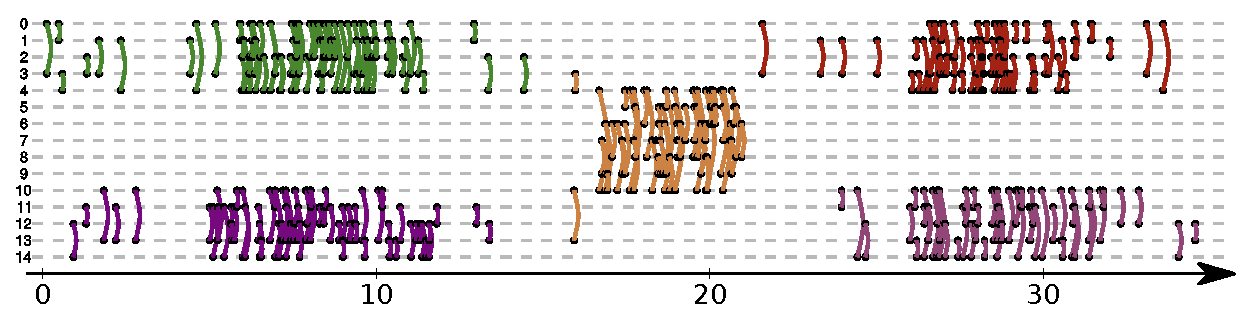
\includegraphics[width=\linewidth]{img/Intro/Dessin_Flot.eps}
            \vspace*{1cm}
            \flushleft{Soutenue publiquement le 11 Octobre 2016 devant le jury composé de}\\[2ex]
            \flushleft{\begin{tabular}{llll}
                    \emph{Rapporteurs:} &  David \textsc{Chavalarias} & Chargé de recherche, \textsc{CNRS}\\
                     &  Jean-Loup \textsc{Guillaume} & Professeur, Université de la Rochelle\\
                     \emph{Examinateurs:} &  Bertrand \textsc{Jouve} & Directeur de recherche, \textsc{CNRS} \\
                     &  Catherine \textsc{Matias} & Directeur de recherches, \textsc{CNRS} \\
                     &  Gilles \textsc{Tredan} & Chargé de recherches, \textsc{CNRS}\\
                     &  Véronique \textsc{Serfaty} & Responsable scientifique, DGA  \\
                     \emph{Directeurs:} &  Clémence \textsc{Magnien} & Directrice de recherche, \textsc{CNRS}\\
                     &  Matthieu \textsc{Latapy} & Directeur de recherche, \textsc{CNRS}\\
                \end{tabular}
            }
      
 \end{titlepage}
% - - - - - - - fin de la page de garde

%\begin{titlepage}
%\begin{center}
%
%{\scshape\LARGE \univname\par}\vspace{1.5cm} % University name
%\textsc{\Large Doctoral Thesis}\\[0.5cm] % Thesis type
%
%\HRule \\[0.4cm] % Horizontal line
%{\huge \bfseries \hspace*{-0.22cm} \ttitle\par}\vspace{0.4cm} % Thesis title
%\HRule \\[1.5cm] % Horizontal line
% 
%\begin{minipage}[t]{0.4\textwidth}
%\begin{flushleft} \large
%\emph{Auteur:}\\
%\authorname % Author name - remove the \href bracket to remove the link
%\end{flushleft}
%\end{minipage}
%\begin{minipage}[t]{0.4\textwidth}
%\begin{flushright} \large
%\emph{Directeurs:} \\
%\supname % Supervisor name - remove the \href bracket to remove the link  
%\end{flushright}
%\end{minipage}\\[3cm]
%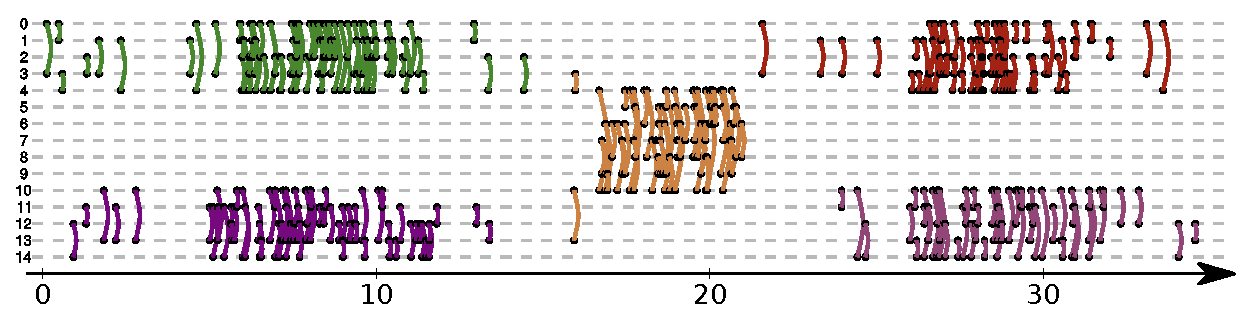
\includegraphics[width=\linewidth]{img/Intro/Dessin_Flot.eps}
%%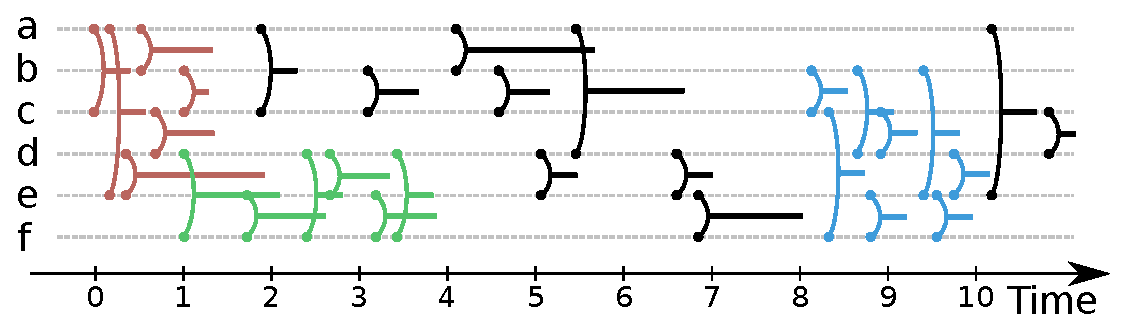
\includegraphics[width=\linewidth]{img/GroupeDense/GroupExample/Zone_dense.eps}
% 
%\large \textit{A thesis submitted in fulfillment of the requirements\\ for the degree of \degreename}\\[0.3cm] % University requirement text
%\textit{in the}\\[0.4cm]
%\groupname\\\deptname\\[2cm] % Research group name and department name
% 
%{\large \today}\\[4cm] % Date
%%\includegraphics{Logo} % University/department logo - uncomment to place it
% 
%\vfill
%\end{center}
%\end{titlepage}


%\begin{acknowledgements}
\addchaptertocentry{Remerciements} % Add the acknowledgements to the table of contents

%The acknowledgments and the people to thank go here.

%\end{acknowledgements}


\tableofcontents


\mainmatter % Begin numeric (1,2,3...) page numbering

\pagestyle{thesis} % Return the page headers back to the "thesis" style

%\listoftodos
\adjustmtc

\chapter*{Introduction}
\addstarredchapter{Introduction}

\chapter{État de l'art sur la détection de communautés et les réseaux dynamiques}
\minitoc
Au cours de cette thèse, nous étudions deux axes de recherches liés aux graphes qui sont orthogonaux.
D'une part, il s'agit de la détection de structures dans les graphes et plus particulièrement de communautés.
Un communauté est un sous-ensemble de n\oe uds de manière à ce qu'ils soient fortement connectés.
Il n'existe cependant aucune définition exact et la notion de communauté fortement connectée dépends du contexte et de la méthode.
Malgré cette définition floue, des structures communautaires ont été trouvées dans de nombreux graphes dans plusieurs domaines tel que les réseaux de [..] \REF.
Ces notions de communautés et les méthodes de détection sont définies dans la section~\ref{sec:intro_communaute}.\\

D'autre part, il a été observé que la modélisation d'un réseau sous la forme d'un graphe peut poser problème notamment quand le réseau change au cours du temps \REF.
Face à ce problème plusieurs extensions de la théorie des graphes ont été proposées et elles sont résumées dans la section~\ref{sec:intro_extension_temporelle}.



\section{Communauté dans les graphes}
\label{sec:intro_communaute}

Ce champs de recherche est très vaste et il est illusoire de vouloir énumérer les méthodes existantes dans ce domaine car les caractéristiques voulues d'une communauté peuvent varier~\cite{Coscia2011}.
Il y a tout de même deux grandes catégories qui permette de séparer les méthodes existantes.
Dans ces deux catégories, les méthodes existantes cherchent à capturer 
des communautés fortement connectées mais elles différent sur ce qu'elles capturent comme structures communautaires.
Les communautés d'une structure communautaires peuvent être disjointes, c'est-à-dire que deux communautés n'ont aucun n\oe uds en commun, ou alors recouvrantes, c'est-à-dire que deux communautés peuvent avoir plusieurs n\oe uds en commun.
Dans le premier cas, on parle de partition des n\oe uds et dans le second on parle de couverture ou partitions chevauchantes de n\oe uds.
Dans ces deux cas, il y a également une contrainte sur le fait que tout les n\oe uds doivent appartenir à au moins une communauté.
C'est deux structures sont correspondent à deux visions possibles de l'organisation d'un graphe et du réseau sous-jacent.
Nous présentons ces deux catégories dans les sous-sections suivantes.

\subsection{Parititons de n\oe uds}
Afin de mieux comprendre ce que peux capturer une parition de n\oe uds, il est plus facile de partir d'un exemple.
Dans l'étude de Stehlé~\emph{et al.}~\cite{Stehle2011}, des enfants d'une école primaire ont eu pendant 2 jours des capteurs enregistrant lorsque deux enfant sont à une distance de moins de 1m50 l'un de l'autre.
Ce dispositif permet de mesurer les interactions entre élèves et de construire le graphe des relations entre élève à l'école.
Une illustration du graphe obtenu est visible dans la figure~\ref{fig:ecole_primaire}.
La classe de chaque élève est également connue.
Comme chaque élève appartient à une et une seule classe, les classes forment une partition des élèves.
Cette partition est une bonne structure communautaire car on remarque que les élèves d'une même classe parle beaucoup entre eux mais ils parlent peu entre élèves de classes différentes.
Cela se remarque particulièrement bien pour la classe 3A.
Il existe beaucoup de liens entre les élèves de la classe 3A et aucun entre eux et les élèves de la classe 5A par exemple.

\begin{figure}
\centering
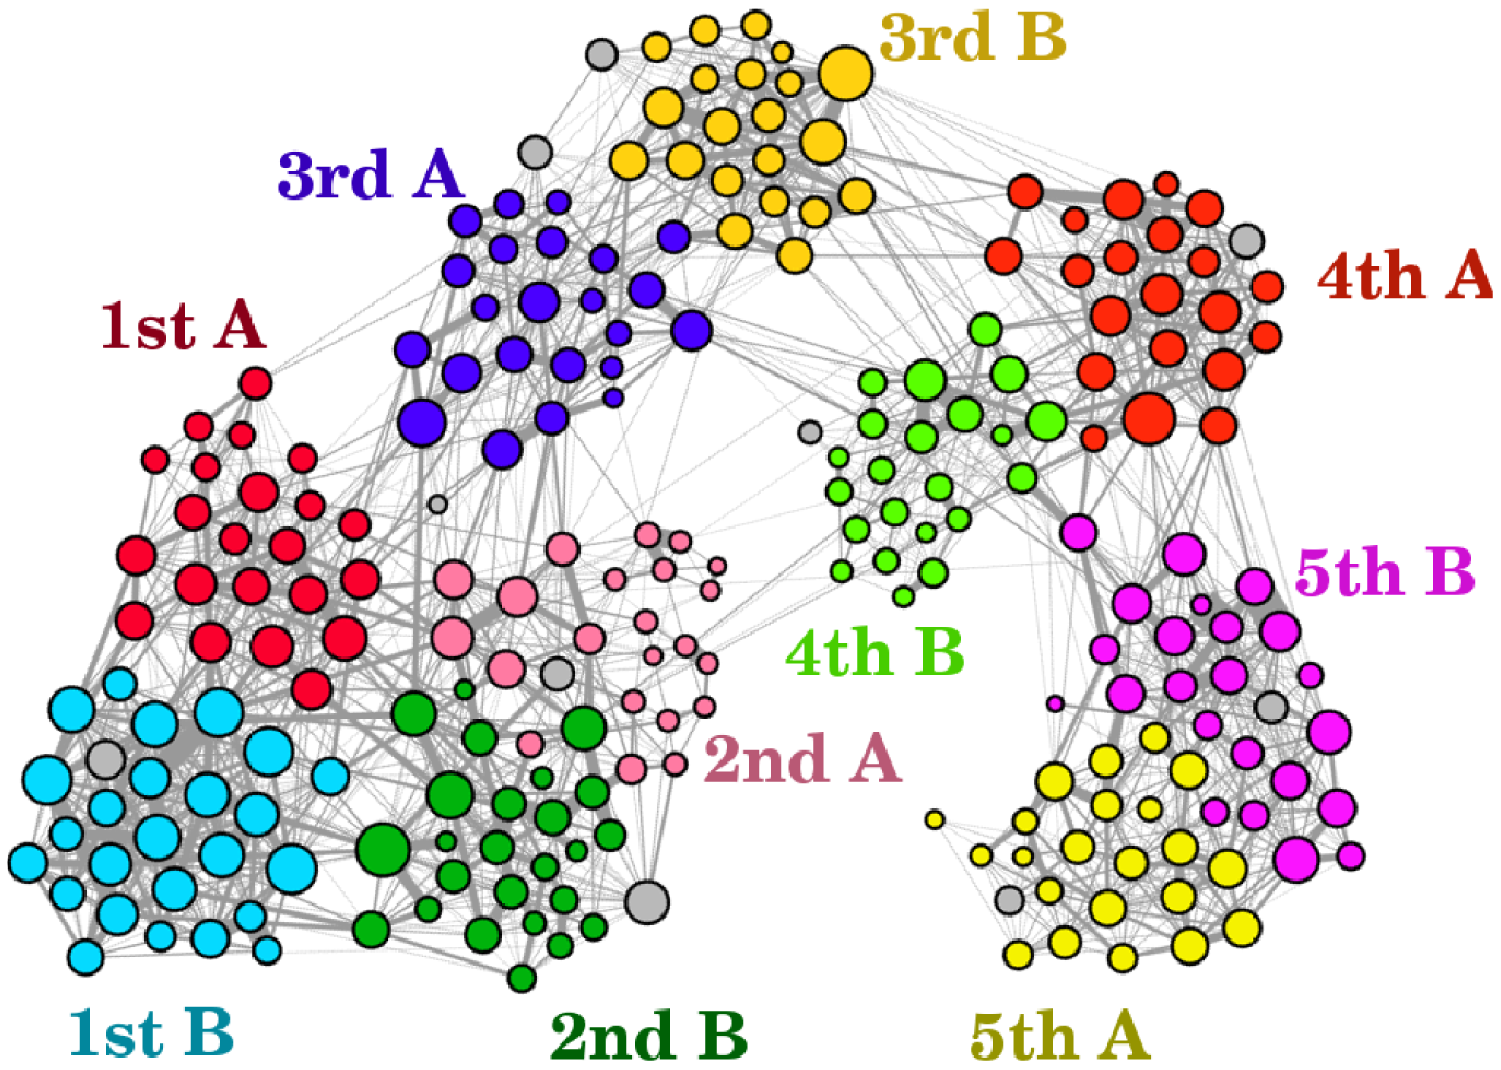
\includegraphics[width=0.7\linewidth]{img/Intro/ecole_primaire}
\caption{Graphe de contact des enfant d'une école primaire. L'épaisseur du lien représente la durée de communication entre deux élèves. La couleur représente la classe de chaque élèves. Les professeurs sont en gris.\protect\footnotemark}
\label{fig:ecole_primaire}
\end{figure}
\footnotetext{Image provenant de \url{http://journals.plos.org/plosone/article?id=10.1371/journal.pone.0023176}.}

Afin de capturer des partitions de n\oe uds, beaucoup de méthodes existent.
Il y a d'ailleurs régulièrement des état de l'art qui sont publiés~\cite{Fortunato2010,Plantie2013a, Malliaros2013a, Harenberg2014a}

limite modu: \cite{Fortunato2007} extension \cite{Reichardt2006, Delvenne2010}
modularité~\cite{Newman2004}, infomap, SBM \cite{Holland1983a}, LPA, Surprise

lien entre SBM et modularité\cite{Newman2016}
\subsection{Couverture de n\oe uds}
\label{subsec:cover}
Etat de l'art.
\cite{Danisch2012, Kanawati2014, Xie2013,Bandyopadhyay2015}

infomap, SBM, MMSBM~\cite{Ball2011,Airoldi2008} , LPA, fonction de qualité locale (conductance, cohésion), fonction de proximité


\subsection{Comapraison}
ARI, NMI, F1-score, Omega index.


\section{Extension temporelle des graphes}
\label{sec:intro_extension_temporelle}

application:
Mobile: \cite{Aledavood2015}
Diffusions \cite{Backlund2014}
Face-to-face interaction: \cite{Barrat2013,Asur2009}
Communauté TVG: \cite{Bassett2013,Bazzi2014}
\subsection{snapshot}
snap\cite{Asur2009,Bassett2013,Bazzi2014} + fenetre glissante
\subsection{TVG/Evolving}
\cite{Casteigts2011}
\subsection{Flots de liens}
Formalisation algébric \cite{Batagelj2015}.
Le formalisme de flot de liens est défini plus en profondeur dans le chapitre~\ref{chap:def_flot}.

temps intrinseque.
\cite{Albano2006}


\chapter{État de l'art sur la détection de communautés et les réseaux dynamiques}
\chaptermark{État de l'art}
\minitoc
\label{chap:etat_art}
Dans cette thèse, nous étudions deux axes de recherches liés aux graphes qui sont orthogonaux.
Avant de présenter ces deux axes de recherches dans les sections~\ref{sec:intro_communaute} et \ref{sec:intro_extension_temporelle}, nous revenons dans la section~\ref{sec:def_graphe} sur quelques définitions et notations utiles pour manipuler des graphes.

Le premier axe de recherche est la détection de structures dans les graphes et plus particulièrement de communautés.
Une communauté est une partie du graphe telle qu'il existe beaucoup de liens à l'intérieur de la communauté et moins avec le reste du graphe.
Cependant aucune définition ne fait l'unanimité.
La notion de communauté dépend du contexte et de la méthode.
Malgré cette définition floue, des structures communautaires ont été trouvées dans de nombreux graphes dans plusieurs domaines tels que le réseau constitué des régions du cerveau \cite{DeReus2014}, un réseau de distribution d'eau \cite{DiNardo2015} et un réseau d'interactions d'animaux \cite{Farine2015}.
Ces notions de communautés et les méthodes de détection sont définies dans la section~\ref{sec:intro_communaute}.

Le second axe de recherche est la prise en compte du temps dans la théorie des graphes.
La première approche fût de complètement ignorer l'information temporelle et de considérer que tous les liens apparaissent en même temps; on parle alors de graphe agrégé.
Cependant, la modélisation d'un réseau sous la forme d'un graphe agrégé manque de pertinence, lorsque le réseau change trop au cours du temps~\cite{Holme2015b}.
Si tel est le cas, certaines structures présentes dans le graphe peuvent n'être que des artefacts de l'agrégation temporelle.
Imaginons par exemple un graphe représentant les alliances politiques dans un pays sur une longue période.
Si toutes les alliances politiques sont agrégées, alors les personnes changeant de parti politique seront faussement considérées comme influentes car connectées à plusieurs partis alors qu'elles peuvent ne plus avoir de contact dans leur ancien parti.
Ainsi, il n'est plus possible d'observer la répartition des alliances politiques dans ce genre de réseau si l'agrégation temporelle est trop importante~\cite{Mucha2010}.

Si on prend en compte le temps, alors il est possible de détecter des structures plus fines que dans le cas statique.
En effet, il devient possible de détecter des instants où l'organisation générale change~\cite{Rosvall2010}, de comprendre quels sont les instants où un n\oe ud est important~\cite{Magnien2015,Costa2015,Takaguchi2016}, ou bien de détecter des groupes temporels~\cite{Cazabet2010}.
Pour ce faire, plusieurs extensions de la théorie des graphes ont été proposées et elles sont présentées dans la section~\ref{sec:intro_extension_temporelle}.


\section{Définition dans les graphes}
\label{sec:def_graphe}

Un graphe $G$ est défini par un couple $(V, E)$  où $V$ est un ensemble de n\oe uds et $E \subseteq V \times V$ est un ensemble de liens; chaque lien étant une paire de n\oe uds.
Sauf mention contraire, nous considérons des graphes non-orientés, c'est-à-dire pour toute paire de n\oe uds $u,v \in V$, les liens $(u,v)$ et $(v,u)$ sont équivalents.
Nous considérons également uniquement des liens non-pondérés, c'est-à-dire qu'un lien est soit présent soit absent.
Enfin, nous ne considérons que des graphes simples, c'est-à-dire qu'il n'existe au maximum qu'un seul lien entre deux n\oe uds et aucun lien de la forme $(u,u)$.
Ceci est en opposition avec les graphes multiples où il peut exister plusieurs liens entre deux n\oe uds.

Par convention, nous notons $n=|V|$ le nombre de n\oe uds et $m=|E|$ le nombre de liens.
On suppose en général que $V=\{1, ..., n\}$.
Il est possible de représenter un graphe $G$ par une matrice carrée $A$ de taille $n$ où l'élément $A_{i,j} \ \forall i,j \in V$ est égale à $1$ si un lien relie les n\oe uds $i$ et $j$ et $0$ sinon.
Avec ces notations, nous définissons les notions suivantes:
\begin{description}
\item[Degré] Le degré d'un n\oe ud $i$, noté $d_i$, est égal au nombre de liens reliés à $i$: $d_i = \sum_{j \in V} A_{i,j}$;
\item[Densité] La densité, $\delta(G)$ d'un graphe est la probabilité que deux n\oe uds pris au hasard soient reliés par un lien: $\delta(G)=\dfrac{2m}{n(n-1)}$;
\item[Degré moyen] Le degré moyen $\tilde{\delta}(G)$ est égal à : $\tilde{\delta}(G)=\dfrac{2m}{n}$;
\item[Chemin] Un chemin dans un graphe est une suite de liens $((u_1,v_1),...,(u_k,v_k))$ de telle sorte que $v_{i}=u_{i+1} \ \forall i \in [1,k-1]$;
\item[Graphe connexe] Les n\oe uds d'un graphe sont dit connexes s'il existe un chemin entre toutes les paires de n\oe uds du graphe;
\item[Composante Connexe] Une composante connexe est un ensemble de n\oe uds $V'\subseteq V$ qui est connexe et maximal, c'est-à-dire qu'il n'est pas possible d'ajouter un n\oe ud dans $V'$ tel que $V'$ soit connexe;
\item[Arbre] Un arbre est le graphe connexe le moins dense et il est constitué de $n-1$ liens pour $n$ n\oe uds;
\item[Clique] Une clique, aussi appelée graphe complet, est le graphe le plus dense et elle est composée de $\dfrac{n(n-1)}{2}$ liens pour $n$ n\oe uds;
\item[Sous-graphe] Un graphe $G'=(V',E')$ est un sous-graphe de $G$ si et seulement si $V' \subseteq V$ et $E' \subseteq E$;
\item[Graphe induit] Le graphe induit par un ensemble de n\oe uds $V' \subseteq V$ est défini par $V'$ et $E'= E \cap (V' \times V')$.  
\end{description}



\subsection{Groupes, partitions et couvertures}
En plus des n\oe uds et des liens, nous manipulons également des ensembles de liens et des ensembles de n\oe uds.
Par convention, notons $X \subseteq V$ un ensemble de n\oe uds et $Y \subseteq E$ un ensemble de liens.
Nous listons les notations utilisées dans le tableau~\ref{tab:notation_groupe_noeuds}.


\begin{table}
  \centering
    \begin{tabular}{|c|c|}
     \hline
    \rule[-1ex]{0pt}{4ex} Notation & Définition \\
  \hline
		\hline
		\rule[-1ex]{0pt}{4ex}$V(Y)=\{u,\ \exists (u,v) \in Y \}$ & n\oe uds induits par les liens de $Y$\\
		\hline
        \rule[-1ex]{0pt}{4ex}$n_X=|X|$ & nombre de n\oe uds dans $X$\\
        \hline
        \rule[-1ex]{0pt}{4ex} $l_{in}(X)=|E \cap (X \times X)|$ & nombre de liens entre les n\oe uds de $X$\\
        \hline
        \rule[-1ex]{0pt}{4ex} $l_{out}(X)=|E \cap (X \times V \setminus X)|$ & nombre de liens entre les n\oe uds de $X$ et de $V \setminus X$ \\
        \hline
        \rule[-1ex]{0pt}{4ex} $l(X)=l_{in}(X)+l_{out}(X)$ & nombre de liens reliés aux n\oe uds de $X$\\
        \hline
        \rule[-1ex]{0pt}{4ex} $d_{in}(u,X)=|\{(u,v) \in E,\ v \in X\}|$ & nombre de liens que partagent $u$ avec $X$ \\
        \hline
        \rule[-1ex]{0pt}{4ex} $d_{in}(X)=\sum_{u \in X} d_{in}(u,X)=2l_{in}(X)$ & somme des degrés internes des n\oe uds dans $X$ \\
        \hline
        \rule[-1ex]{0pt}{4ex} $d_{out}(u,X)=|\{(u,v) \in E,\ v \in V \setminus X\}|$ & nombre de liens que partagent $u$ avec $V \setminus X$ \\
        \hline
       \rule[-1ex]{0pt}{4ex}  $d_{out}(X)=\sum_{u \in X} d_{out}(u,X)=l_{out}(X)$ & somme des degrés externes des n\oe uds dans $X$ \\
        \hline
        \rule[-1ex]{0pt}{4ex}  $d(X)=d_{in}(X)+ d_{out}(X)$ & somme des degrés des n\oe uds dans $X$ \\
        \hline
    \end{tabular}
    \caption{Liste des notations utilisées pour un ensemble de n\oe uds $X$ et un ensemble de liens $Y$.}
         \label{tab:notation_groupe_noeuds}
\end{table}%


\paragraph{Partitions et couvertures}
Nous définissons ici les structures de partitions et de couvertures appliquées au cadre spécifique des graphes.
Une partition de n\oe uds, $\mathcal{V}$, est un ensemble d'ensembles de n\oe uds: $\mathcal{V}= \{V_1,..., V_k\}$ tel que $\forall i \in [1,k]\ V_i \subseteq V$ et tel que:
\begin{enumerate}
\item La partition \emph{recouvre} l'ensemble des n\oe uds: $\bigcup_{i} V_i = V$.
\item Les ensembles de n\oe uds sont disjoints: $V_i \cap V_j = \emptyset\ \forall i,j \in [1,k],\ i \neq j$.
\end{enumerate}
Afin de manipuler une partition, nous définissons $\mathcal{V}(u)=V_i$ si et seulement si $u \in V_i$.
\bigskip

Une couverture est une extension des partitions car elle relâche la contrainte sur l'intersection.
Ainsi, une couverture de n\oe uds, $\mathcal{V}$, est aussi un ensemble d'ensembles de n\oe uds.
L'union des ensembles doit également être égale à $V$ mais en revanche deux ensembles de n\oe uds peuvent partager un n\oe ud: $\exists i,j \in [1,k],\ i \neq j\ V_i \cap V_j \neq \emptyset$.
Une couverture est parfois aussi appelée partition chevauchante.

Nous avons détaillé les notions de partitions et couvertures de n\oe uds mais les mêmes définitions valent pour les partitions et couvertures de liens.
Enfin, il existe d'autres structures possibles comme les structures non-exhaustives où un élément peut n'appartenir à aucun ensemble.

\subsection{Comparaison de partitions et couvertures}
Il est souvent utile de pouvoir comparer deux partitions ou deux couvertures entre elles.
Le but est de calculer une similarité entre deux structures de telle sorte que la similarité est égale à $1$ si les deux structures sont identiques et qu'elle soit égale à $0$ ou $-1$ si elles sont complètement différentes.
Il existe pour ce faire des méthodes tirant parti de la structure d'ensembles et celles provenant de la théorie de l'information.

\paragraph{Approches ensemblistes}
\label{def:graphe_comparaison}
Il est possible de comparer deux ensembles $X$ et $Y$ en utilisant l'indice de Jaccard, $\mathbb{J}(X,Y) = \dfrac{|X \cap Y|}{|X \cup Y|}$, ou le \emph{F1 score} $F_1(X,Y) = 2\dfrac{|X \cap Y|}{|X| + |Y|}$.
Avec l'indice de Jaccard ou le \emph{F1 score}, il est possible de mesurer la similarité entre deux partitions $\mathcal{X}$ et $\mathcal{Y}$:
\begin{equation}
sim(\mathcal{X},\mathcal{Y})=\frac{1}{|\mathcal{X}|}\sum_{X \in \mathcal{X}}\max_{Y\in \mathcal{Y}}\mathbb{J}(X,Y).
\end{equation}

Avec cette formulation, la similarité n'est pas symétrique.
C'est pourquoi la formule suivante lui est souvent préférée:

\begin{equation}
sim_{moy}(\mathcal{X},\mathcal{Y}) = \dfrac{sim(\mathcal{X},\mathcal{Y})+sim(\mathcal{Y},\mathcal{X})}{2}
\end{equation}
Il existe d'autres méthodes pour symétriser la similarité, \emph{e.g.} la moyenne harmonique.
Cette méthode peut s'appliquer indifféremment aux partitions et aux couvertures.

Il existe également le \emph{Rand Index}~\cite{Rand1971} qui lui ne s'applique qu'aux partitions.
Il mesure le nombre de paires de n\oe uds qui sont classées de la même manière dans les deux partitions; c'est à dire pour deux n\oe uds $u$ et $v$ soit $\mathcal{X}(u)=\mathcal{X}(v)$ et $\mathcal{Y}(u)=\mathcal{Y}(v)$ soit $\mathcal{X}(u)\neq \mathcal{X}(v)$ et $\mathcal{Y}(u)\neq \mathcal{Y}(v)$.
Plus formellement, soient $a_{11}$ le nombre de paires de n\oe uds de telle sorte qu'ils soient dans le même ensemble dans les deux partitions, $a_{00}$ le nombre de paires de n\oe uds de telle sorte qu'ils soient dans des ensembles différents dans les deux partitions et $a_{10}$ (resp. $a_{01}$) le nombre de paires de n\oe uds de telle qu'ils soient dans le même ensemble dans $\mathcal{X}$(resp. $\mathcal{Y}$) et dans deux ensembles différents dans $\mathcal{Y}$ (resp. $\mathcal{X}$).
Avec ces notations, le \emph{Rand Index} est défini de la manière suivante:

\begin{equation}
RI(\mathcal{X},\mathcal{Y}) = \dfrac{a_{11} + a_{00}}{a_{11}+a_{01}+a_{10}+ a_{00}}
\end{equation}
Il se peut que, par chance, deux partitions classent de la même manière une paire de n\oe uds, notamment à cause de $a_{00}$.
C'est pourquoi une version ajustée du \emph{Rand Index} (ARI) a été proposée~\cite{Hubert1985}.
Le \emph{Rand Index} et sa version ajustée permettent de comparer des partitions.
Porumbel~\emph{et al.}~\cite{Porumbel2011} ont proposé l'Omega Index qui est une extension de l'ARI pour les couvertures.

\paragraph{Approche venant de la théorie de l'information}
On peut considérer que l'assignation d'un élément à un ensemble est une variable aléatoire.
Dans ce cas, la probabilité d'un élément d'être dans un ensemble $X \in \mathcal{X}$ est $P(X)= n_X/|V|$.
De manière similaire, la probabilité jointe est $P(X,Y) = |X \cap Y|/|V|$.
Avec ces définitions, il est possible de calculer l'entropie d'une partition, $H(\mathcal{X})$, l'entropie conditionnelle, $H(\mathcal{X}|\mathcal{Y})$ et l'information mutuelle $I(\mathcal{X},\mathcal{Y})$.
Cette dernière est définie par $I(\mathcal{X}, \mathcal{Y}) = H(\mathcal{X}) - H(\mathcal{X}|\mathcal{Y})$.
L'entropie, $H(\mathcal{X})$, et l'entropie conditionnelle, $H(\mathcal{X}|\mathcal{Y})$, sont définies dans le sens de Shanon par: 
\begin{equation}
H(\mathcal{X}) = - \sum_{X \in \mathcal{X}} P(X)\log(P(X)),\quad H(\mathcal{X}|\mathcal{Y}) = -\sum_{X \in \mathcal{X},\ Y \in \mathcal{Y}} P(X, Y) \log \dfrac{P(X,Y)}{P(Y)}.
\end{equation}
Afin de normaliser l'information mutuelle, Danon~\emph{et al.}~\cite{Danon2005a} ont défini l'information mutuelle normalsée ($NMI_{shanon}$):
\begin{equation}
 NMI_{shanon}(\mathcal{X},\mathcal{Y}) = \dfrac{2I(\mathcal{X},\mathcal{Y})}{H(\mathcal{X})+H(\mathcal{Y})}.
\end{equation}

Lancichinetti \emph{et al.} l'ont par la suite étendue pour prendre en compte les couvertures~\cite{Lancichinetti2009d}.
Le choix de la normalisation dans le cas chevauchant semble cependant toujours ouvert~\cite{McDaid2011,Zhang2015c}.

\resume{
Il est intéressant de noter que la littérature sur la comparaison de structures est assez restreinte comparé à celle sur la détection de communautés.
En effet, il semble qu'uniquement 3 similarités soient couramment utilisées: la similarité se basant sur Jaccard, l'Omega index et la NMI.
Tout les indices de similarité ont été étendus aux couvertures de manière assez convaincantes.
Il est également important de noter l'existence d'implémentations librement accessible de la majeure partie de ces métriques\, \footnote{\url{https://github.com/aaronmcdaid/Overlapping-NMI}}\,\footnote{\url{http://scikit-learn.org/stable/modules/clustering.html\#clustering-evaluation}}.
}


\section{Communautés dans les graphes}
\label{sec:intro_communaute}

Ce champ de recherche est très vaste et il est illusoire de vouloir énumérer les méthodes existantes dans ce domaine car elles sont extrêmement nombreuses et les caractéristiques voulues d'une communauté peuvent varier selon le contexte~\cite{Leskovec2008,Coscia2011,Yang2015,Jeub2015}.
Les méthodes se séparent tout de même en plusieurs catégories selon qu'elles capturent une partition ou une couverture de n\oe uds.
Ces deux structures correspondent à deux visions possibles de l'organisation d'un graphe et du réseau sous-jacent.
Nous présentons ces deux catégories dans les sous-sections suivantes.
Il existe également une troisième catégorie qui est la détection de communautés sous la forme de partitions de liens que nous traitons dans le chapitre~\ref{chap:Expected_Node}.

\subsection{Parititons de n\oe uds}
\label{subsec:Part_noeuds}
Afin de mieux comprendre ce que peut capturer une partition de n\oe uds, il est plus facile de partir d'un exemple.
Dans l'étude de Stehlé~\emph{et al.}~\cite{Stehle2011}, des enfants d'une école primaire ont eu pendant 2 jours des capteurs enregistrant lorsque deux enfants sont à une distance de moins de 1 mètre 50.
Ce dispositif permet de mesurer les interactions entre élèves et de construire le graphe des relations à l'école.
Un lien existe entre deux élèves s'ils ont interagi au moins une fois ensemble.
Une illustration du graphe obtenu est visible dans la figure~\ref{fig:ecole_primaire}.
La classe de chaque élève est également connue.
Comme chaque élève appartient à une et une seule classe, les classes forment une partition des élèves.
Cette partition est une bonne structure communautaire car on remarque que les élèves d'une même classe interagissent beaucoup entre eux mais peu avec les élèves des autres classes.
Cela se remarque particulièrement bien pour la classe $3A$.
Il existe beaucoup de liens entre les élèves de la classe $3A$ mais aucun avec les élèves de la classe $5A$ par exemple.

\begin{figure}
\centering
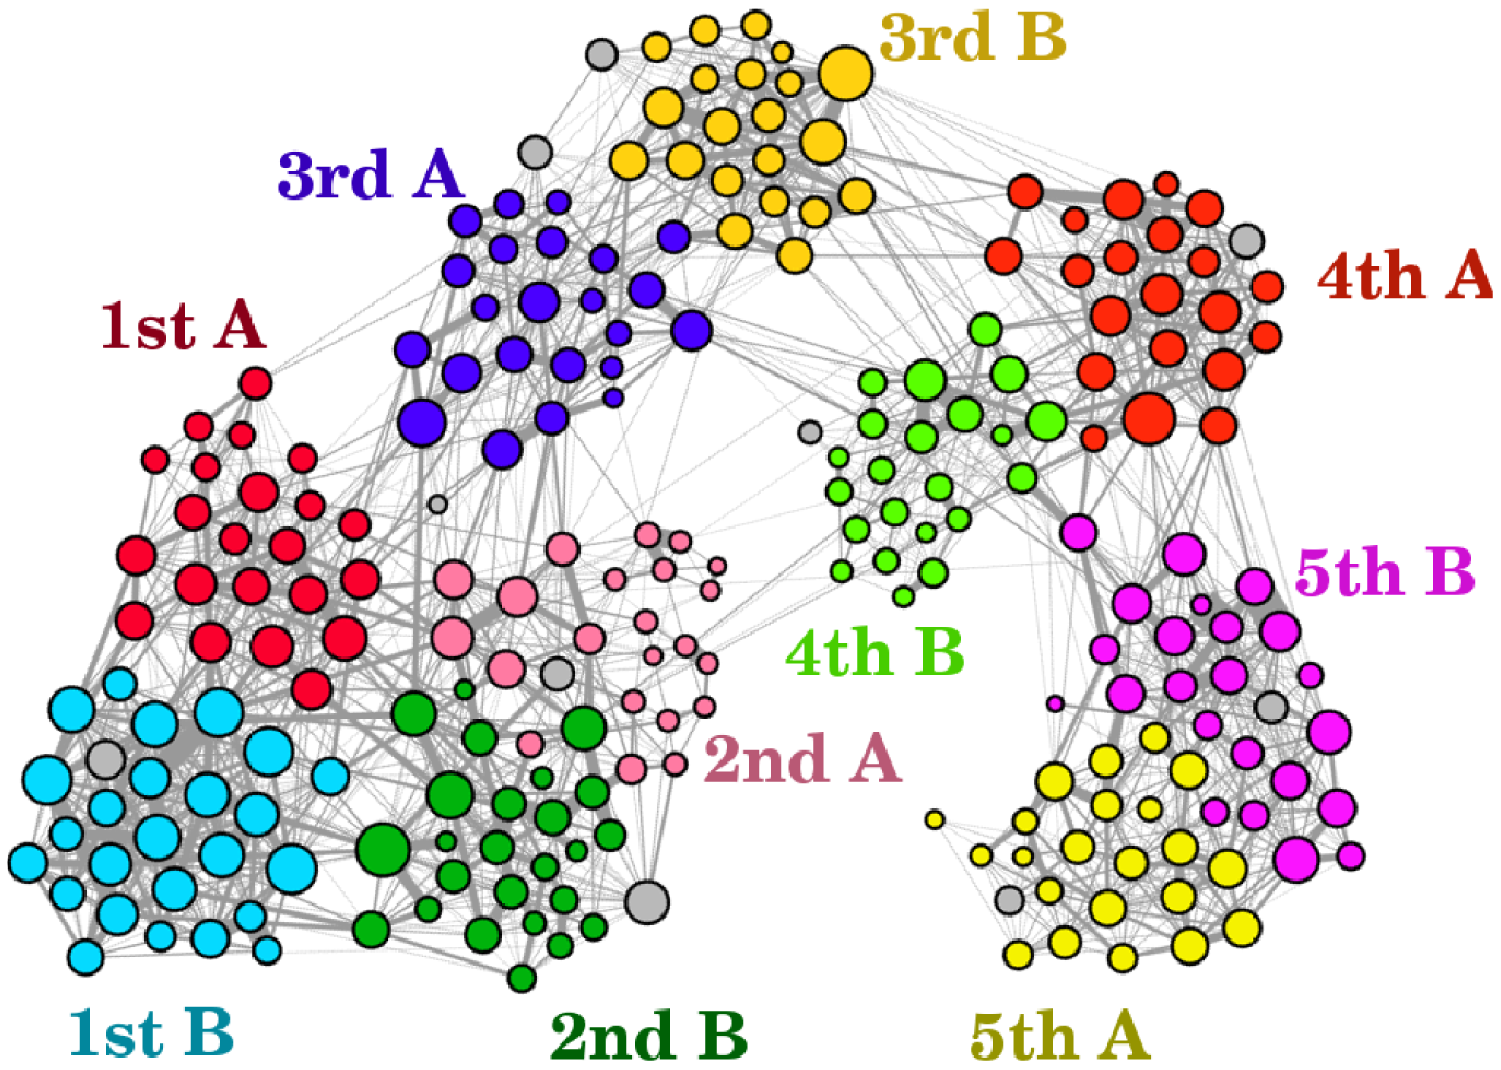
\includegraphics[width=0.6\linewidth]{img/Intro/ecole_primaire}
\caption{Graphe de contact des enfants d'une école primaire. L'épaisseur du lien représente la durée de communication entre deux élèves. La couleur représente la classe de chaque élève et la taille représente le degré du n\oe ud. Les professeurs sont en gris.\protect\footnotemark}
\label{fig:ecole_primaire}
\end{figure}
\footnotetext{Image provenant de \url{http://journals.plos.org/plosone/article?id=10.1371/journal.pone.0023176}.}

Afin de capturer des partitions de n\oe uds, beaucoup de méthodes existent.
Il y a d'ailleurs régulièrement des états de l'art qui sont publiés~\cite{Fortunato2010,Plantie2013a, Malliaros2013a, Harenberg2014a}.
Afin d'aider le lecteur, nous détaillons ici quelques unes des méthodes les plus utilisées.

\subsubsection{Méthodes utilisant un modèle}
\label{def:Modularite}
Comme une communauté est souvent définie comme devant être très densément connectée, le problème est de trouver une fonction capable d'évaluer la qualité d'une communauté.
Pour ce faire, il faut définir une métrique qui mesure la densité, \emph{e.g.} le nombre de liens dans un groupe.
Puis, il est nécessaire de définir comment évaluer cette métrique.

Il est possible d'utiliser une métrique en la normalisant par ses bornes minimum et maximum.
Avec une métrique normalisée entre $0$ et $1$, un groupe est alors considéré comme très connecté si son évaluation est supérieure à un certain seuil.
Par exemple, le nombre de liens entre $n$ n\oe uds peut être normalisé par le nombre de liens dans un arbre et dans une clique de taille $n$. 
Cette approche n'est cependant pas adaptée pour la recherche de communautés car elle ne tient pas compte de la structure du graphe\,\footnote{Cette approche est plus appropriée dans la recherche des groupes les plus denses~\cite{Balalau2015}.}.
Prenons l'exemple du graphe constitué d'une unique clique.
Dans ce graphe, tout groupe de n\oe uds est également une clique et par conséquent tout groupe de n\oe uds a une évaluation parfaite de $1$.
Chaque groupe serait donc une très bonne communauté selon cette évaluation.
Or, le graphe constitué d'une unique clique ne possède pas de structure communautaire contrairement au graphe dans la figure~\ref{fig:ecole_primaire}.
Il est donc nécessaire de trouver une autre approche.

\bigskip

Plutôt que de normaliser une métrique par ses valeurs minimum et maximum, il est intéressant de considérer l'écart à une valeur attendue.
L'idée est la suivante: quelle serait la valeur attendue de la métrique considérée si le graphe n'avait pas de structure communautaire.
Le problème est alors de "retirer" la structure communautaire du graphe ou bien de définir un ensemble de graphes similaires au graphe initial mais n'ayant pas de structure communautaire.
Ce processus définit alors ce qu'on appelle un \emph{modèle nul}.
Détecter des communautés se traduit ainsi en trouver des groupes qui s'éloignent du modèle nul où il n'existe pas de communauté.

Ce changement est astucieux car il est relativement aisé de définir des graphes n'ayant pas de structure.
Il suffit de créer des graphes complètement aléatoires~\cite{Erdos1959} où les liens du graphes sont tirés de manière uniforme.
Afin que les graphes aléatoires puissent être comparés au graphe initial, des contraintes sont généralement ajoutées et donnent lieu à différents modèles nuls.
Le premier modèle nul de graphe est celui de Erdös-Rényi~\cite{Erdos1959} où le nombre de liens et le nombre de n\oe uds des graphes aléatoires doivent être les mêmes que dans le graphe initial.
Un autre modèle très couramment utilisé est le modèle de configuration~\cite{Bender1978a}.
Dans ce modèle, la distribution des degrés est également fixe.
Le modèle de configuration est utilisé car il a été observé que les graphes provenant de données réelles ont une distribution des degrés très éloignée d'une distribution uniforme.
C'est pourquoi l'ajout de la contrainte sur les degrés permet de considérer des graphes plus proche du graphe initial. 
Il existe bien évidement d'autres modèles possibles considérant d'autres contraintes~\cite{Newman2009}.

\paragraph{Modularité}
La modularité~\cite{Newman2004} est une fonction qui associe à chaque partition de n\oe uds une valeur entre $-1$ et $1$.
Plus la valeur de modularité d'une partition est élevée, plus la partition est censée capturer une bonne structure communautaire.
La modularité est définie de la manière suivante pour une partition $\mathcal{C}$:

\begin{equation}
Q(\mathcal{C}) = \dfrac{1}{2m}\sum_{i,j \in V} \left(A_{ij} - \dfrac{d_id_j}{2m}\right)\ \delta_{\mathcal{C}(i)=\mathcal{C}(j)} \ ,
\end{equation}
où $\delta_{C(i)=C(j)}$ est égale à $1$ si $i$ et $j$ sont dans la même communauté et $0$ sinon.
Il s'agit pour deux n\oe uds d'une même communauté de comparer la présence ou l'absence d'un lien, $A_{ij}$, à la probabilité que ces n\oe uds soient reliés dans le modèle de configuration, $\dfrac{d_id_j}{2m}$.
L'idée sous-jacente est que les n\oe uds d'une communauté devraient partager plus de liens qu'espéré dans le modèle de configuration.
De très nombreux travaux ont par la suite étudié les caractéristiques de la modularité et son optimisation.
Tout d'abords, il a été montré que l'optimisation de la modularité est un problème NP-Complet~\cite{Brandes2007}.
Il est donc nécessaire de recourir à des heuristiques afin de trouver rapidement une partition proche de l'optimum.
Parmi l'ensemble des algorithmes existants, l'algorithme de Louvain~\cite{Blondel2008a} est un des plus rapide.
Il existe également des variantes de cet algorithme~\cite{Huang2015,Traag2015c}.

D'autres travaux se sont attachés à l'étude de la modularité.
Il a été montré que la modularité souffre du problème de \emph{résolution limite}~\cite{Fortunato2007,Lancichinetti2011} car le modèle de configuration présuppose une répartition uniforme des tailles des communautés.
Il a par ailleurs été montré que la modularité n'offre pas de maximum clair et que beaucoup de partitions différentes ont des évaluations proches~\cite{Good2010}.
Pour répondre à ces problèmes, il existe différentes variantes de la modularité~\cite{Reichardt2006,Delvenne2010}.

%\paragraph{Surprise}
%La fonction Surprise~\cite{Aldecoa2011,Traag2015b} est une autre fonction de qualité qui se base quant à elle sur le modèle de Erdös-Rényi pour évaluer la surprise d'observer un groupe de n\oe uds relié par $l$ liens.

\paragraph{\emph{Stochastic Block Model}}
Nous avons défini précédemment la notion de modèle nul permettant de se comparer à l'absence de communautés.
Il est également possible de modéliser une structure communautaire puis de vérifier \emph{a posteriori} si ce modèle pourrait être à l'origine du graphe observé.
Le problème de détection de communauté est alors un problème d'inférence qui est traité avec des outils statistiques tel que le \emph{stochastic block model} (SBM)~\cite{Holland1983a,Nowicki2001}.
L'idée derrière le SBM est la suivante: la probabilité que deux n\oe uds soient reliés dépend uniquement de leur groupe respectif.
Si le graphe a une structure communautaire\,\footnote{Il est également possible de représenter d'autres type de structures.}, alors deux n\oe uds d'une même communauté devraient avoir une forte chance d'être connecté.
\`A l'inverse, deux n\oe uds de deux communautés différentes devraient avoir une probabilité assez faible d'être connecté.
Le SBM est défini par de nombreux paramètres: le nombre de groupes, l'assignation d'un groupe à chaque n\oe ud et les probabilités d'interactions entre les groupes.
Avec un jeu de paramètres donné, il est possible de calculer la vraisemblance que ce jeu de paramètres soit à l'origine du graphe.
Trouver une partition de n\oe uds dans ce contexte est alors équivalent à trouver le jeu de paramètre qui est le plus vraisemblablement à l'origine du graphe.


Dans le SBM, tout les n\oe uds sont considérés comme équivalents en particulier vis-a-vis du degré ce qui n'est pas le cas dans beaucoup de graphes provenant de données réelles.
C'est pourquoi une version tenant compte du degré des n\oe uds a été proposée: le Degree-corrected Stochastic Block Model (DSBM)~\cite{Karrer2011}.
Enfin d'après des récents travaux~\cite{Newman2016}, il semblerait que le DSBM et l'optimisation de la modularité soient liés.

\subsubsection{Méthodes utilisant des marches aléatoires}
Il existe d'autres approches que celles utilisant un modèle nul ou un modèle génératif.
Notamment, il y a les méthodes utilisant les marches aléatoires \cite{Pons2005,Rosvall2008}.
Ces méthodes tirent parti du fait que si une communauté est densément connectée alors un marcheur aléatoire devrait y rester assez longtemps.
En particulier, la méthode Infomap~\cite{Rosvall2008} repose sur une idée très élégante qui est la suivante.
Une partition de n\oe uds est une carte du graphe et, en ce sens, elle doit aider sa lecture.

Une carte est efficace si elle permet de mieux comprendre l'objet d'étude en réduisant sa complexité.
Dans une carte d'un pays, les départements découpent l'espace en zones disjointes et la majorité des routes se trouvent à l'intérieur des départements.
Dans une carte, il est courant qu'un nom de ville soit unique dans un département mais qu'un même nom puisse être utilisé dans plusieurs départements.
De plus, un voyageur se déplaçant aléatoirement sur les routes a peu de chance de sortir d'un département.
Pour décrire, \emph{a posteriori}, l'ensemble des villes traversées par ce voyageur, il suffit alors de donner le département initial puis la liste des villes visitées.
Il n'est pas nécessaire de répéter le département pour chaque ville si le voyageur n'en est pas sorti.
En ce sens, la découpe d'un pays en département permet de réduire la complexité de la description du voyage.
Il s'agit donc d'un problème lié à la théorie de l'information et de sa compression.
De manière similaire, Rosval~\emph{et al.} utilise des marcheurs aléatoires se déplaçant sur les n\oe uds du graphe et les communautés comme zones du graphe.
Si les communautés sont bien formées, alors les marcheurs aléatoires restent bloqués à l'intérieur des communautés et la description de leur marche est courte.
La longueur de cette description devient alors la signature de la partition et plus la signature est courte, meilleure la partition est.

Le phénomène de résolution limite a également été étudié dans le cadre de Infomap~\cite{Kawamoto2015}.
Il semble que cet effet existe également dans Infomap mais qu'il soit beaucoup moins prononcé.

\paragraph{Autres méthodes}
Il existe bien d'autres méthodes pour détecter des communautés en tant que partition de n\oe uds.
Il y a les méthodes spectrales~\cite{Donetti2004,Mitrovic2009} qui se basent sur les vecteurs propres de la représentation d'un graphe sous la forme d'une matrice.
De manière moins formelle, il existe également les méthodes de propagation de labels (LPA)~\cite{Raghavan2007a,Li2014c}.
Dans ces méthodes, chaque n\oe ud a initialement un label puis à chaque itération chaque n\oe ud prend comme label un des labels de ses voisins.
En général, un n\oe ud prend comme label celui qui est le plus présent parmi ses voisins.
Au bout d'un certain nombre d'itérations ou une fois à l'équilibre, il ne reste que quelques labels dans le graphe et ils représentent les communautés.


\resume{Il existe de très nombreuses méthodes pour la détection de communautés en tant que partition de n\oe uds. Il semble que les méthodes d'optimisation de \textbf{modularité}, la méthode \textbf{infomap} et  les \textbf{Stochastic Block Model} soient les plus utilisées dans la littérature.}

\subsection{Couverture de n\oe uds}
\label{subsec:cover}
Jusqu'à maintenant, nous avons considéré les communautés comme des partitions de n\oe uds.
Or, les partitions sont très restrictives et ne peuvent pas capturer toutes les situations possibles.
Prenons l'exemple d'un graphe reflétant des interactions entre personnes.
Il existe des communautés qui sont disjointes comme le travail et la famille mais bien souvent des personnes appartiennent à plusieurs groupes, voir l'exemple dans la figure~\ref{fig:ex_overlap_communaute}.
Ainsi le groupe des personnes faisant du sport et le groupe des personnes travaillant ensemble peuvent ne pas être disjoints.
Si tel est le cas, alors il n'est plus possible de représenter ces communautés avec une partition.
Il est nécessaire de manipuler une couverture de n\oe uds.
Ainsi dans l'exemple dans la figure~\ref{fig:ex_overlap_communaute}, les n\oe uds rouges appartiennent à deux groupes au lieu d'un seul.

\begin{figure}
	\centering
	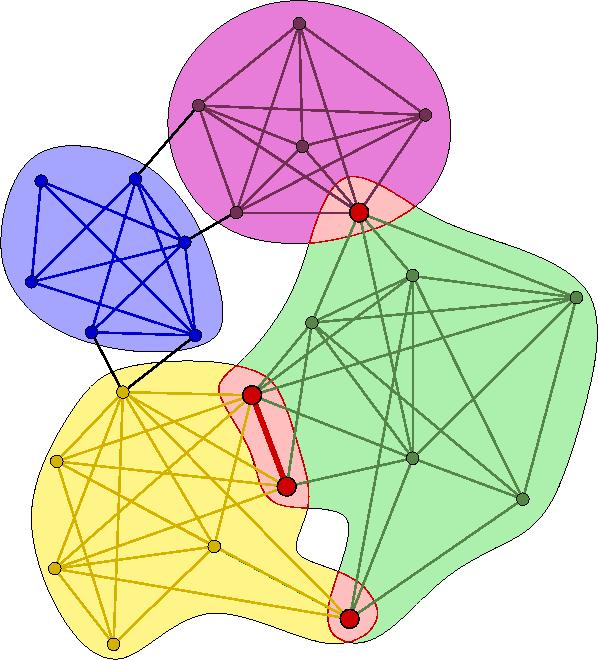
\includegraphics[width=0.31\linewidth]{img/Intro/Illustration_of_overlapping_communities.jpg}
	\caption{Exemple graphe avec une structure communautaire chevauchante représentée par les couleurs\,\protect\footnotemark.}
	\label{fig:ex_overlap_communaute}
\end{figure}
\footnotetext{Image provenant de \url{https://en.wikipedia.org/wiki/Clique_percolation_method}.}

Une fois encore, la littérature est très vaste dans ce domaine et nous ne ferons pas une liste exhaustive des méthodes existantes.
Il existe de nombreux état de l'art dans le domaine~\cite{ Kanawati2014, Xie2013,Bandyopadhyay2015, Hric2014a}.

Une des premières méthodes de détection de couverture de n\oe uds est la \emph{Clique Percolation Method} (CPM)~\cite{Palla2005}.
L'algorithme CPM repose sur le principe de transitivité qui serait à l'origine des communautés: si $i$ et $j$ sont reliés par un lien, alors un n\oe ud $k$ qui serait relié à $i$ aurait une forte chance d'être également connecté à $j$.
Il s'agit de la formalisation du proverbe "Les amis de mes amis sont mes amis".
Si ce principe est réellement à l'origine des communautés, alors les communautés doivent être composées de plusieurs cliques.
C'est pourquoi CPM cherche l'ensemble des cliques d'une taille $k$ donnée\,\footnote{En général, $k$ est compris entre 3 et 5 pour des raisons de coût de calcul.} puis fusionne toutes les cliques qui partagent suffisamment de n\oe uds, en général $k-1$. 
Comme cette méthode est relativement coûteuse, Kumpula \emph{et al.}~\cite{Kumpula2008} ont repris le même mécanisme en optimisant le mode de calcul.

\subsubsection{Extension des méthodes de détection de partitions}

La majorité des méthodes existantes pour les partitions ont été adaptées pour manipuler les couvertures de n\oe uds.
Il existe notamment plusieurs extensions de la modularité~\cite{Shen2009,Nicosia2009}.
Cependant ces extensions ne reposent plus sur un modèle nul car elles introduisent des termes de normalisation.
Par conséquent, ces extensions sont beaucoup moins utilisées que la modularité initiale.

\paragraph{Stochastic Block Model}
En revanche, le SBM s'adapte très bien aux couvertures de n\oe uds.
Une extension du SBM est le Mix-Membership Stochastic Block Model (MMSBM)\cite{Airoldi2008} qui permet à un n\oe ud d'avoir plusieurs groupes.
Dans~\cite{Gopalan2013a}, les auteurs utilisent la même méthode mais en échantillonnant le graphe initial afin de réduire le coût de calcul.
Il existe d'autres méthodes à base de modèle génératif~\cite{Ball2011,Yang2013}.
Ces méthodes se basent sur des graphes d'affiliations~\cite{BreigerRonald1974}.
Un graphe d'affiliation est un graphe biparti entre les n\oe uds d'une part et les communautés de l'autre part.
Dans la méthode de Ball~\emph{et al.}~\cite{Ball2011}, ce graphe d'affiliation est pondéré et la pondération représente la propension d'un n\oe ud à créer des liens dans un groupe donné tandis que pour Yang~\emph{et al.} il s'agit du facteur d'appartenance du n\oe ud au groupe.
Une fois le graphe d'affiliation défini, il est nécessaire de savoir recréer la matrice d'adjacence et, en ce sens, ces méthodes se rapprochent des méthodes de factorisation en matrices non-négatives~\cite{Lee1999}.
Le but de la factorisation non-négative d'une matrice donnée est d'être capable de trouver deux matrices dont les entrées sont non-négatives telles que leur combinaison permette de retrouver la matrice initiale.

Jusque récemment ce genre de technique généralisant le SBM ne pouvait s'appliquer qu'à des graphes relativement petits.
Cependant les méthodes récentes~\cite{Gopalan2013a, Yang2013} arrivent à traiter des graphes ayant énormément de liens, de l'ordre $10^{9}$ à $10^{12}$ liens.



\paragraph{Propagation de label}
Des méthodes ont étendu la propagation de label aux couvertures de n\oe uds~\cite{Gregory2010,Xie2011}.
Le principal changement est qu'un n\oe ud ne stocke plus un unique label mais soit plusieurs labels soit des fréquences d'apparition de labels.
Ainsi à la fin de l'algorithme, il suffit de choisir les labels les plus fréquents.
Cependant ce mécanisme de propagation change radicalement l'idée initiale.
En effet, la diffusion d'un label n'est plus directement contrainte par la diffusion des autres labels.
Dans cette nouvelle configuration, il est possible qu'un label soit présent dans tous les n\oe uds.
De plus selon les auteurs de ces méthodes, des communautés non connexes peuvent apparaître ce qui nécessite l’ajout d’un mécanisme de \emph{post-processing}.


\paragraph{Infomap}
Il s'agit sûrement avec le SBM de la méthode étant la moins "déformée" par l'adaptation aux couvertures de n\oe uds.
En effet, il suffit de relâcher la contrainte sur le fait qu'un n\oe ud n'appartienne qu'à un seul groupe.
Il est toujours possible de décrire un trajet par un nom de groupe puis une liste de n\oe uds visités dans le même groupe.
Ainsi, la notion de longueur de description est toujours valide dans ce contexte.
Ce travail d'extension a été fait par Esquivel~\emph{et al.}~\cite{Esquivel2011}.

\subsubsection{Méthodes utilisant des communautés égocentrées}
On a vu avec la modularité qu'il est assez difficile de définir une fonction de qualité évaluant une couverture de n\oe uds en fonction des caractéristiques des groupes.
C'est pourquoi certaines méthodes s'affranchissent complètement de fonction de qualité globale et se concentrent sur des propriétés locales.
Dans cette philosophie, il y a les méthodes se basant sur des fonctions de proximité et celle utilisant des fonctions de qualité locales.

Dans le premier cas, le but est de mesurer la proximité entre tous les n\oe uds et un n\oe ud appelé égo.
Puis une fois les n\oe uds ordonnés selon leur similarité, il suffit de définir une coupe pour séparer les n\oe uds appartenant à la même communauté que l'égo et les autres.
Le choix de la coupe se fait, en général, en fonction de la présence de forte décroissance de la similarité.
Pour obtenir une couverture de n\oe uds, il est nécessaire d'appliquer ce processus égocentré sur plusieurs égos.
Danisch~\emph{et al.}~\cite{Danisch2012} utilise une méthode de diffusion pour mesurer la similarité, alors que Whang~\emph{et al.}~\cite{Whang2013} utilise le \emph{Personalized Page Rank}.
Ces méthodes ne sont cependant pas à même d'évaluer les communautés qu'elles trouvent.
\bigskip

D'autres méthodes prennent le contre-pied des méthodes de proximité en utilisant des fonctions de qualité locales.
Il s'agit d'algorithmes qui initialement considèrent de très petites communautés puis essayent de les étendre itérativement en ajoutant des n\oe uds.
Afin de ne pas étendre un groupe indéfiniment, un ajout n'est fait que s'il améliore la fonction de qualité locale.
Ainsi dans ce type d'algorithme, il y a deux critères important:
le choix des communautés initiales et le critère d'évaluation.
Dans la majorité des cas, chaque n\oe ud constitue initialement une communauté. 
OSLOM\cite{Lancichinetti2011a} diffère de cette situation car OSLOM utilise comme point de départ une partition trouvée par l'algorithme de Louvain ou par infomap.

Les fonctions de qualité applicables sont très nombreuses et nous n'en mentionnerons que trois.
Tout d'abord, il est possible d'utiliser le degré relatif~\cite{Luo2008} d'un groupe comme critère.
Il s'agit du ratio entre le nombre $l_{in}$ de liens internes à un groupe de n\oe uds et le nombre de liens total $l_{in}+l_{out}$: $ \dfrac{l_{in}}{l_{in}+l_{out}}$.
En effet, plus le degré relatif est élevé, plus le groupe est dense comparé à son voisinage et plus il a de fortes chances d'être une bonne communauté. 
Cette formulation est assez proche de la conductance ou coupe normalisée~\cite{Shi2000}:
\begin{equation}
\phi =\dfrac{l_{out}}{\min \left( 2(l_{in}+l_{out}),m-2(l_{in}-l_{out}) \right) }
\end{equation}

Ces deux notions se rapportent à la notion de densité vis-à-vis de leur voisinage.
Il est également possible d'évaluer une communauté locale par rapport aux nombre de triangles présents dans la communauté.
C'est ce que mesure la cohesion~\cite{Friggeri2011} pour un groupe de taille $k$: 
\begin{equation}
cohesion=\dfrac{\Delta_3}{ {k \choose 3} } \times \frac{\Delta_3}{\Delta_3+\Delta_2},
\end{equation}
où $\Delta_3$ est le nombre de triangles dont les 3 n\oe uds sont à l'intérieur du groupe et $\Delta_2$ est le nombre de triangles dont uniquement 2 n\oe uds sont à l'intérieur du groupe.

D'autres méthodes d'initialisation ainsi que fonctions de qualité sont détaillées dans l'article de Kanawati~\cite{Kanawati2014}.
Ces méthodes semblent très prometteuses car elles permettent de traiter efficacement de très grands graphes tout comme les algorithme de propagations de label mais elles profitent des fonctions de qualité locales qui permettent d'une certaine manière d'évaluer le résultat obtenu.



\resume{
La littérature sur la détection de couverture de n\oe uds est encore très récente.
Il est donc délicat de commencer à tirer des conclusions.
Cependant, il semble que les extensions de la modularité ne soient pas réellement capables de trouver des couvertures de n\oe uds.
En plus d'infomap, c'est surtout les méthodes utilisant des modèles génératifs et celles utilisant des fonctions de qualité locales qui semblent les plus à même de capturer des couvertures de n\oe uds pertinentes.
Les modèles génératifs ne semblent en effet plus limités à de petits graphes.
Les méthodes utilisant des fonctions de qualité locales sont quant à elle très rapides et le choix de la fonction de qualité permet de s'adapter au contexte.
}


\section{Extension temporelle des graphes}
\label{sec:intro_extension_temporelle}

Les graphes sont utilisés pour représenter une situation ou résoudre un problème réel.
Dans la section précédente, nous nous sommes attachés à présenter une partie des méthodes considérant le problème de la détection de communautés recouvrantes ou non.
Cependant toutes ces méthodes reposent sur la validité de la représentation du problème par un graphe.
Cette hypothèse est justifiée dans énormément de cas mais elle ne l'est plus lorsque l'objet d'étude évolue beaucoup.

Afin d'illustrer ce propos, nous nous appuyons sur le même exemple de réseau de personnes que nous avons présenté dans la sous-section~\ref{subsec:Part_noeuds} et qui est illustré dans la figure~\ref{fig:ecole_primaire}.
Dans cet exemple, deux élèves sont reliés dans le graphe s'ils ont interagi au moins une fois au cours de la capture.
Comme la capture n'a duré que deux jours, il est fort probable que les élèves n'aient pas changé d'habitude durant la capture.
En étudiant le graphe agrégé, il est possible de mettre en avant l'organisation générale des élèves mais déjà de l'information a été perdue.
En effet, il n'est pas possible de différencier le comportement observé le matin de celui observé le soir car l'ensemble des interactions sont agrégées dans le graphe.
Ce n'est pas tout, imaginons que la capture ait duré plusieurs mois voire plusieurs années.
Dans ce cas de figure, il ne sera plus possible de dégager un comportement général des élèves car il aura changé durant ce laps de temps.
En particulier, de nouveaux groupes d'amis se seront formés et d'autres auront disparu.
Tout ces changements impactent le graphe agrégé et tendent au fur et à mesure à le rapprocher d'une clique ce qui le rend complètement inexploitable.
Le temps est donc une dimension qu'il est nécessaire de prendre en compte.

Le domaine de l'épidémiologie est un très bon exemple de l'importance du temps.
Un modèle épidémique représente la propagation d'une maladie dans une population en fonction des contacts qui existent.
Il est donc tout naturel de s'appuyer initialement sur un graphe où les n\oe uds représentent des personnes et les liens représentent les interactions entre personnes.
En plus du graphe, il est nécessaire d'ajouter l'état de chaque n\oe ud, \emph{e.g.} sain ou infecté.
Ainsi, un n\oe ud sain ne peut devenir infecté que s'il est relié à un n\oe ud infecté dans le graphe.
Ce genre de modèles met donc en avant un chemin de diffusion, \emph{e.g.} une suite de personnes transmettant la maladie à l'autre.

Afin d'illustrer ce phénomène, les premiers travaux~\cite{Vespignani2008}
s'appuient sur un graphe d'interactions de personnes agrégeant toute l'information temporelle.
Or, la prise en compte du temps dans ce contexte est primordiale car il est possible que le chemin d'infections simulé dans le graphe agrégé ne soit pas réalisable si l'on prend en compte le temps.
Imaginons 3 personnes $A$, $B$, $C$ tel que $A$ et $B$ interagissent à l'instant $1$, $B$ et $C$ interagissent à l'instant $2$.
Dans le graphe agrégé, il est possible pour $C$ d'infecter $A$ via $B$ alors que dans la réalité cela n'est pas possible.
L'ajout du temps impacte donc fortement les résultats obtenus dans le contexte épidémiologique et ce phénomène est d'ailleurs très étudié~\cite{Gauvin2015a,Karsai2011,Jo2014,Horvath2014,Holme2014a,Scholtes2014,Perotti2014a}.

Une fois reconnue l'importance du temps, il est nécessaire de trouver un nouveau formalisme étendant la théorie des graphes pour en tenir compte.
Nous présentons maintenant différentes extensions possibles de la théorie des graphes, dans les sous-sections~\ref{subsec:perte_info} et \ref{subsec:pasperte_info}.
Nous détaillons également comment la recherche de communautés se transpose dans ces nouveaux formalismes et plus généralement quels sont les problèmes qu'ils permettent de résoudre.
Des états de l'art dans ce domaine ont d'ailleurs déjà été esquissés~\cite{Boccaletti2014,Cazabet2014,hartmann2014clustering}.

\subsection{Extensions avec pertes d'informations temporelles}
\label{subsec:perte_info}
\subsubsection{Séries de graphes}
\begin{figure}[h]
\centering
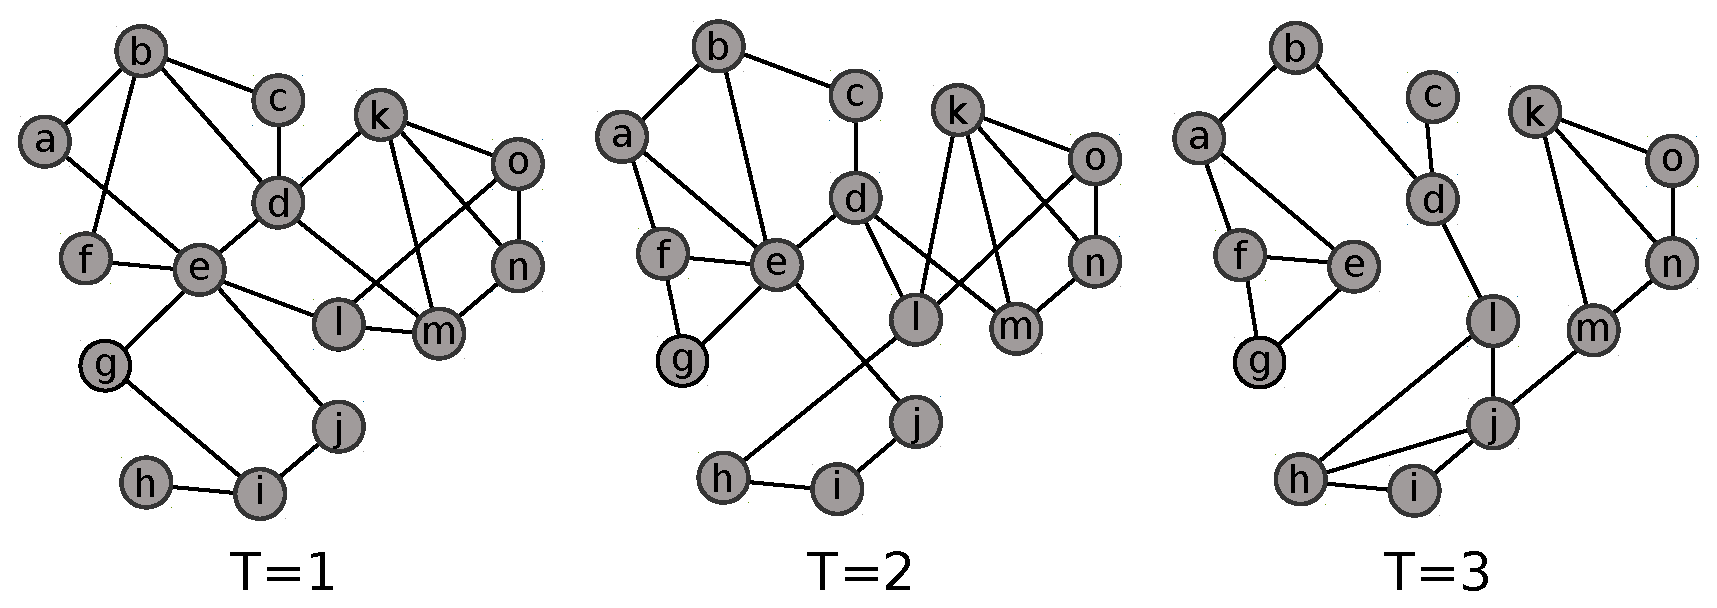
\includegraphics[width=0.8\linewidth]{img/Intro/TVG.eps}
\caption{Exemple de série de graphes sur trois intervalles de temps.}
\label{fig:exemple_TVG}
\end{figure}
La première solution qui a été apportée ne prend le temps en compte que partiellement.
Il s'agit de manipuler une série de graphes où chaque graphe représente le réseau durant un intervalle de temps donné.
Ainsi, il est possible d'appliquer les outils de la théorie des graphes sur chaque intervalle.
Cependant chaque intervalle de temps est représenté par un graphe agrégé.
Il y a donc toujours une perte d'information.
Plus formellement, une série de graphe est définie par $\mathcal{G}=\{G_i\}_{i < T}$ où $T$ est un entier, voir l'illustration~\ref{fig:exemple_TVG}.

Cette définition initiale laisse le choix sur la découpe du temps en intervalle.
Il est possible de choisir des intervalles de tailles égales ou non et disjoints ou chevauchants~\cite{Wang2012}.
Utiliser des intervalles à durée variable permet de mieux tenir compte de la dynamique.
Par exemple lors de l'étude d'interactions de personnes, il est très courant d'observer une très faible activité la nuit et une plus forte la journée.
Un graphe agrégeant ce qui se passe sur un intervalle de 5h sera vide dans le premier cas et peut être trop dense dans le second.
La détection d'intervalle pertinent est donc un vaste sujet de recherche~\cite{Rosvall2010,Krings2012,Ribeiro2013,Caceres2013,Peel2015,de2016detection}.

La notion même de temps est importante.
Albano~\emph{et al.}~\cite{Albano2014} propose d'utiliser une autre mesure que la seconde mais plutôt le nombre de changements comme mesure du temps.
Ainsi, le temps n'avance pas si aucun changement n'a lieu et au contraire il avance beaucoup si énormément de changements apparaissent.
Cette manière de procéder se rapproche des travaux de Lamport~\cite{Lamport1978} dans les systèmes distribués.

\paragraph{Détection de communautés}
Dans ce contexte de série de graphes, il y a eu assez tôt des méthodes de détection de communautés~\cite{Hopcroft2004,Sun2007,Lin2008,Asur2009}.
Il est, en effet, assez naturel d'appliquer une méthode de détection statique sur chaque graphe puis d'essayer de faire du suivi de communautés.
Le suivi de communautés consiste à comprendre comment une communauté donnée évolue, étant donné une série de graphes et une série de partitions.
Palla~\emph{et al.}~\cite{Palla2007} ont été parmi les premiers à décrire les évolutions possibles d'une communauté.
Muni d'indicateurs de similarité tels que l'indice de Jaccard, voir la section~\ref{def:graphe_comparaison}, il est possible de trouver les communautés les plus proches aux instants précédent et suivant.
\`A partir de ces informations, six type d'évolutions d'une communauté sont définis:
\begin{description}
\item[Naissance] Une nouvelle communauté apparait.
\item[Agrandissement] La communauté continue d'exister et s'agrandit.
\item[Fusion] Deux communautés fusionnent pour donner lieu à une nouvelle communauté.
\item[Division] Une communauté se sépare en deux nouvelles communautés à l'étape suivante.
\item[Retrescissement] La communauté continue d'exister mais perd quelques n\oe uds.
\item[Mort] Une communauté cesse d'exister dans les graphes suivants.
\end{description}

Ce type de méthodes souffre souvent de l'instabilité des méthodes de détection~\cite{Aynaud2010,Harenberg2014a}.
Si les partitions changent complètement entre deux graphes consécutifs, alors il est difficile de faire un réel suivi de communautés.
C'est pourquoi des méthodes essayent de forcer une certaine stabilité de la partition en ajoutant un coût de transition~\cite{Chakrabarti2006,Chen2013,Kalavathi2015}.
Une approche détournée pour garder une certaine stabilité est d'utiliser la partition trouvée précédemment comme base de recherche pour l'intervalle suivant~\cite{Lancichinetti2011a}.

Des extensions des Stochastic Block Models ont également été proposées par différents auteurs dans le cadre des séries de graphes.
Yang~\emph{et al.}~\cite{Yang2011} sont parmi les premiers à considérer ce cas de figure.
Ils considèrent que la probabilité d'un lien entre deux communautés est fixe et que ce qui change est l'affiliation des n\oe uds au cours du temps.
Ce processus de changement de communauté suit alors une chaine de markov cachée.
\`A l'inverse, Corneli~\emph{et al.}~\cite{Corneli2016} considèrent une partition de n\oe uds fixe tout au long du temps et c'est l'activité entre deux communautés qui change selon l'intervalle de temps.
Xu~\emph{et al.}~\cite{Xu2014} permettent à l'affiliation et à l'activité entre deux communautés de changer selon l'intervalle de temps.
Cependant, il semblerait que cette relaxation se fasse au dépens de l'identifiabilité des paramètres d'après Matias~\emph{et al.}~\cite{Matias2015}.
Ils ont donc proposé une nouvelle méthode afin de résoudre ce problème.
De plus, leur méthode permet de traiter des séries de graphes pondérés.

\subsubsection{Tenseur 3D}
Les tenseurs 3D ne sont pas en soi différents des séries de graphes.
Il est possible de voir un graphe comme une matrice carrée d'adjacence.
Il est donc normal de concevoir une série de graphes comme un tenseur appartenant à $\mathcal{R}_{nnT}$.
Ce changement de point de vue permet ainsi d'appliquer les méthodes d'algèbre linéaire, notamment la décomposition de tenseur.
C'est la méthode proposée par Gauvin~\emph{et al.}~\cite{Gauvin2014} pour étudier la structure communautaire des interactions d'élèves.
Cependant ce genre de décomposition semble moins expressive que les SBM.


\subsubsection{Graphes multicouches}
\begin{figure}[h]
\centering
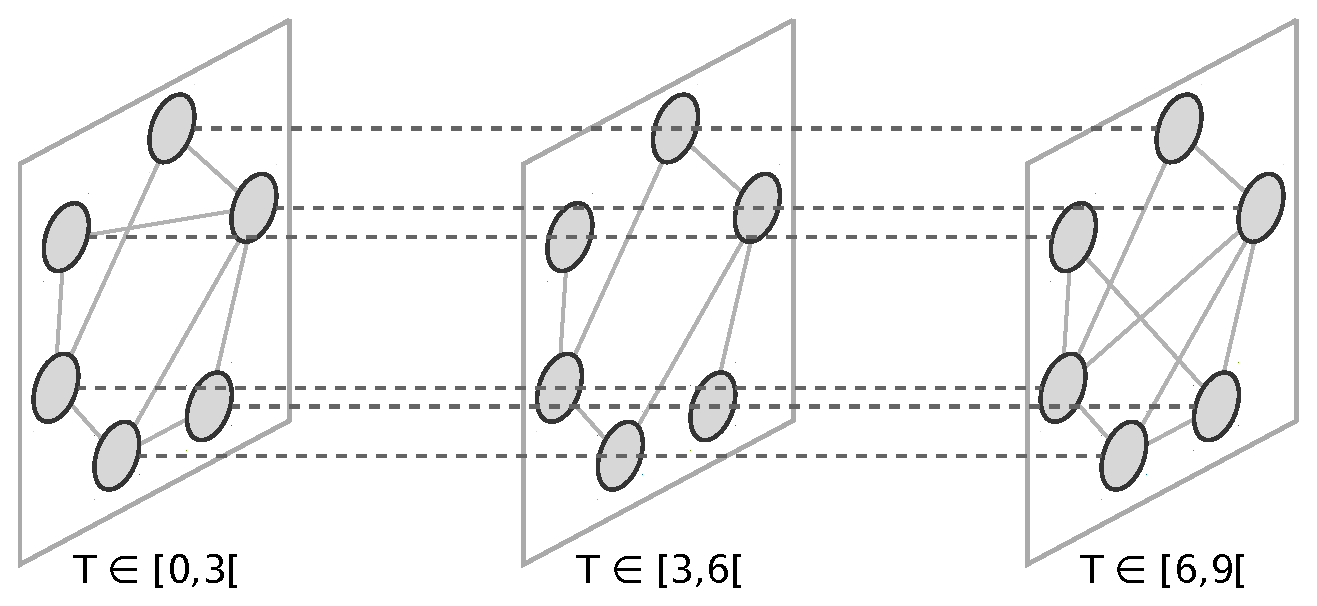
\includegraphics[width=0.7\linewidth]{img/Intro/multiplex.eps}
\caption{Graphe multicouches avec trois couches représentant le temps.
Les liens pleins (resp. pointillés) sont les liens intra-couches (resp. inter-couches).}
\label{fig:exemple_multiplex}
\end{figure}
La construction de graphes multicouches (\emph{multilayer} ou \emph{multiplex}) est proche de l'idée des séries de graphes.
Tout comme les séries de graphes, des n\oe uds et des liens sont créés à chaque intervalle pour représenter ce qui s'est déroulé durant l'intervalle de temps.
Cependant, le graphe multicouches ajoute des liens entre les n\oe uds de deux intervalles, voir l'illustration~\ref{fig:exemple_multiplex}.
Par conséquent, un graphe multicouches est un graphe où il existe deux types de liens, les liens intra-couches et les inter-couches et il existe $T$ répliques d'un même n\oe ud, une par intervalle de temsp.
Les liens intra-couches représentent un connexion entre deux n\oe uds durant un intervalle de temps.
Les liens inter-couches représentent un lien entre deux n\oe uds sur deux intervalles différents.
Ces derniers sont utilisés pour identifier un même n\oe ud sur plusieurs intervalles et sont en général limités à relier deux couches consécutives.

Les graphes multicouches représentent les données évoluant dans le temps mais ils modélisent aussi très bien d'autres situations.
Par exemple, ils permettent de représenter facilement les différents moyens de transport dans une ville où chaque moyen de transport (bus, voiture, métro ...) est représenté par une couche.
Plusieurs travaux~\cite{DeDomenico2013,Kivela2014,Boccaletti2014} décrivent les graphes multicouches et leurs applications.



\paragraph{Détection de communautés}
Grâce au formalisme de graphe multicouches, il est possible de traiter le temps de manière un peu plus fine que dans les séries de graphes car il permet de mieux suivre l'évolution des n\oe uds.
Comme un graphe multicouches est un graphe, il est possible d'adapter les méthodes existantes pour tenir compte des différents types de liens.
C'est le cas d'infomap~\cite{DeDomenico2014}, de la modularité~\cite{Mucha2010,Bassett2013,Bazzi2016} et du SBM~\cite{Stanley,Peixoto2015c}.


\resume{
Les séries de graphes, les tenseurs et les graphes multicouches permettent de prendre en compte le temps tout en autorisant l'utilisation de méthodes conçues sur un graphe statique.
Cette liberté d'utilisation a un coût.
Ces approches reposent sur une découpe du temps en sous-intervalles durant lesquelles le temps n'est plus pris en compte afin d'obtenir un graphe statique.
Or, il peut être délicat de définir ces intervalles de temps.
De plus, la construction des graphes agrégés entraine une perte d'information temporelle et cela impacte la précision temporelle des structures communautaires qui sont manipulables.
Il n'est pas envisageable d'augmenter le nombre d'intervalles de temps car cela induirait d'une part des graphes agrégés avec très peu de liens et d'autre part le temps de calcul serait très fortement impacté.
}

\subsection{Extension sans perte d'information temporelle}
\label{subsec:pasperte_info}
\subsubsection{Graphe temporel}
\begin{figure}[h]
\centering
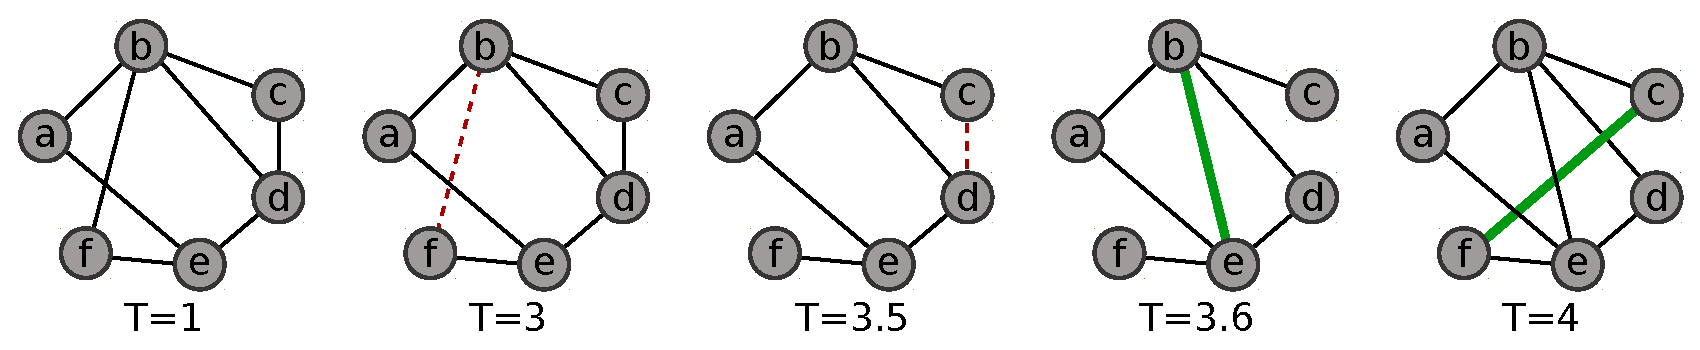
\includegraphics[width=0.9\linewidth]{img/Intro/evolvingGraph.eps}
\caption{Graphe temporel avec des ajouts de lien représentés en trait épais vert et des retraits de lien représentés par des liens pointillés rouge.
}
\label{fig:exemple_evolving}
\end{figure}
Les graphes temporels (\emph{Time Varying Graph} ou \emph{Evolving Graph})
permettent de tenir compte de l'ensemble de l'information temporelle.
Pour cela au lieu de considérer des intervalles de temps, ils considèrent l'ensemble des modifications qui affectent le graphe: les ajouts et retraits de liens.
En pratique, cela revient à considérer sur chaque lien une fonction de présence en fonction de temps qui vaut $1$ à un instant $t$ si le lien existe à cet instant et $0$ sinon.
Ainsi, il est possible de connaitre la structure de graphe à chaque instant.
Ce formalisme est présenté dans différents travaux~\cite{Casteigts2011,Wehmuth2015} et illustré dans la figure~\ref{fig:exemple_evolving}.
Dans cette figure, on voit apparaitre l'ordre de modification du graphe.
Tout d'abord, les liens $(b,f)$ et $(c,d)$ disparaissent puis les liens $(b,e)$ et $(f,c)$ apparaissent chacun leur tour. 

\paragraph{Détection de communautés}
Dans un graphe temporel, une structure de graphe existe à chaque instant.
Il est donc possible de calculer après chaque modification l'évolution d'une métrique.
Par exemple, il est possible de calculer après l'ajout d'un lien le nouveau degré interne des n\oe uds impactés par ce changement.
En fonction de l'évolution de cette métrique, il est alors décidé d'ajouter ou retirer un n\oe ud voire de fusionner deux communautés.
Li \emph{et al.}~\cite{Li2012a} se base sur le nombre de liens que partage un n\oe ud avec les communautés environnantes.
Ainsi, un n\oe ud est toujours dans la communauté avec laquelle il partage le plus de liens.
Shang\emph{et al.}~\cite{Shang2014a}, Cordeiro~\emph{et al.}~\cite{Cordeiro2016} et Sun\emph{et al.}~\cite{Sun2014} se basent sur l'évolution de la modularité.
Cependant, ces approches ne permettent pas l'ensemble des évolutions de communauté possibles, en particulier l'apparition d'une nouvelle communauté.
C'est pourquoi l'évolution de la structure courante peut mener à une structure ayant une faible qualité.
Une autre approche a été proposée par Cazabet~\emph{et al.}~\cite{Cazabet2010} afin d'améliorer l'évolution de la partition.
Ils utilisent une métrique locale basée sur le nombre de chemins de longueur $2$ existant entre un n\oe ud et une communauté.
Après chaque modification, ils considèrent également la possibilité de créer une nouvelle communauté sous la forme d'une petite clique.
Ainsi, ils assurent une meilleure qualité de la partition au cours de l'évolution.


\subsubsection{Flot de liens}
\begin{figure}[h]
\centering
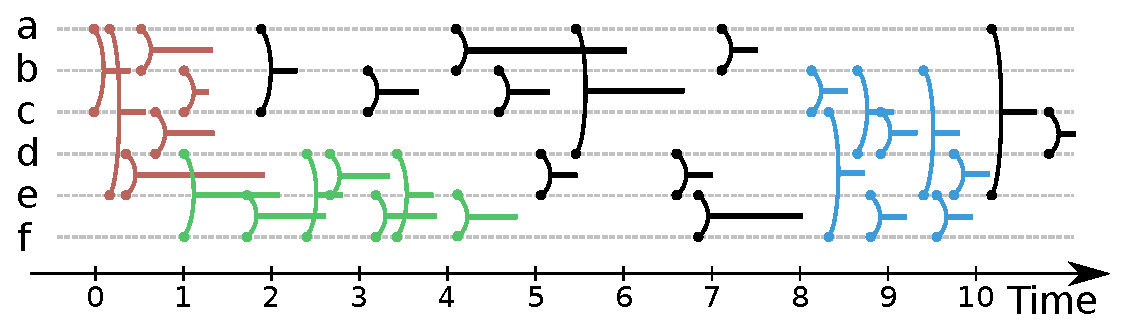
\includegraphics[width=0.9\linewidth]{img/Intro/Flot_de_liens.eps}
\caption{Flot de liens entre $6$ n\oe uds, représentés sur l'axe des ordonnées, au cours du temps représenté sur l'axe des abscisses.
Dans l'exemple, il existe un lien entre $a$ et $b$ durant l'intervalle $[4,6]$.
}
\label{fig:exemple_Flot_de_liens}
\end{figure}
Dans les graphes temporels, toute l'information temporelle est gardée.
Cependant, l'intuition derrière cette méthode est qu'il existe une structure de graphe à chaque instant.
Cette hypothèse n'est pas toujours vérifiée, en particulier lorsque les liens apparaissent et disparaissent très rapidement.
C'est le cas des appels téléphoniques qui durent rarement plus d'une heure ou bien de manière plus frappante avec les SMS et les courriels qui n'ont même pas de durée.
Dans ces contextes, il n'est pas possible de supposer qu'à chaque instant une structure de graphe existe.
Il faut donc un formalisme et des mesures qui s'adaptent à ce contexte.
C'est pour répondre à ce besoin que le formalisme de flot de liens a été pensé.
Le but est de construire un objet ne présupposant aucune structure et qui stocke toute l'information disponible.
Même si le formalisme ne présuppose aucune contrainte structurel, il se peut en revanche que le réseau représenté en ait.
Par exemple dans les télécommunications, une personne ne peut appeler qu'une ou deux personnes en même temps.
Plusieurs travaux~\cite{Holme2013a,Holme2015b,Holme2015e} font un tour d'horizon des méthodes existantes pour étudier les flots de liens qui sont souvent appelés \emph{temporal networks} mais il n'existe, à notre connaissance, qu'un seul travail donnant un fondement théorique solide au flot de liens.
Il s'agit de Batagel~\emph{et al.}~\cite{Batagelj2016} qui se basent sur l'algèbre.
Malheureusement avec une formulation purement algébrique, il semble difficile de transcrire l'ensemble des notions de graphes pour l'instant.
\bigskip

Prenons l'exemple des appels téléphoniques, c'est-à-dire qui parle avec qui à quelle heure et pendant combien de temps.
Un appel peut donc être représenté par un quadruplet $(b,e,u,v)$ où $b$ (res. $e$) est le début (resp. la fin) de l'appel et $u$ et $v$ représentent des personnes.
Il est donc possible de modéliser des appels téléphoniques par un ensemble de quadruplet.
En faisant cela, aucune information n'est perdue et, en ce sens, flots de liens et graphes temporels sont équivalents. 
Cependant, ce changement de perspective induit une réflexion différente selon le formalisme considéré.

Les différences dans les méthodes de représentation des graphes temporels de la figure~\ref{fig:exemple_evolving} et celle des flots de liens de la figure~\ref{fig:exemple_Flot_de_liens} illustrent bien ce changement de perspective, bien que les deux figures ne représentent pas le même réseau.
Dans l'exemple de la figure~\ref{fig:exemple_Flot_de_liens}, les n\oe uds sont représentés sur l'axe des ordonnées et le temps sur l'axe des abscisses.
Un lien dans cette visualisation est représenté par: un arc vertical reliant deux axes de n\oe uds et un trait horizontal représentant la durée du lien.
Ainsi dans l'exemple, il existe un lien entre les n\oe uds $a$ et $b$ dans l'intervalle $[4,6]$.

Dans un graphe temporel, on abordera plus souvent les questions d'évolution de communautés de n\oe uds ou de l'importance d'un n\oe ud.
Dans un flot de liens, on s'intéressera plus souvent au temps nécessaire pour que deux n\oe uds soient de nouveau en contact ou à l'importance d'un lien.
De manière très manichéenne et inexacte, le formalisme de graphe temporel pousse à étudier les relations et leur évolution alors que celui de flot de liens mets plus l'accent sur les interactions et leur dynamique.

\bigskip



Avec ce formalisme, la majorité des travaux sont encore descriptifs car ce type d'objet n'a jamais été étudié sous cet angle.
Il existe de nombreux travaux étudiant le temps séparant l'apparition de deux liens pour un n\oe ud~\cite{Malmgren2008,Malmgren2009}.
Il semblerait que ces temps inter-contacts soient très hétérogènes et que de nombreuses connexions apparaissent dans un faible intervalle de temps suivie de longues durées sans activité.
On parle alors de temps inter-contact \emph{bursty}.
Les effets des temps inter-contacts sur les phénomènes de diffusions et de marches aléatoires sont très étudiés~\cite{Karsai2011,Karsai2012a,Starnini2012b,Rocha2013}.
Il semble cependant ne pas y avoir de conclusion définitive sur le sujet car la diffusion peut être accélérée ou ralentie par les temps inter-contacts selon la structure sous-jacente.

Il existe également quelques méthodes qui s'intéressent plus à la structure des flots de liens.
Des études~\cite{Kovanen2011a,Kovanen2013a} s'intéressent à la présence de motifs.
Un motif dans un graphe est un petit sous-graphe comme le triangle qui est l'un des motifs les plus étudiés.
Dans les flots de liens, le temps est également pris en compte dans les motifs.
Il y a donc plusieurs variantes temporelles d'un même motif dans un graphe.
Prenons l'exemple d'un chemin entre quatre n\oe uds $A$, $B$, $C$ et $D$ qui est représenté dans le graphe par  $\{(A,B), (B,C), (C,D)\}$.
Dans un flot de liens, il existe deux variantes à ce motif soit
$\{(t_1,A,B), (t_2,B,C), (t_3,C,D)\}$ soit $\{(t_1,A,B), (t_2,C,D), (t_3,B,C)\}$ avec $t_1<t_2<t_3$.
Dans un cas,  une information peut être propagée au fur et à mesure de $A$ vers $D$ tandis que dans l'autre ce n'est pas possible.
L'étude de la fréquence d'apparition de ces motifs dans le cas temporel permet d'observer si le flot de liens a une structure particulière. 



\paragraph{Détection de structures}
Il existe peu de méthodes détectant des structures décrivant l'ensemble d'un flot de liens.
Rozenshtein~\emph{et al.}~\cite{rozenshtein2014} se penchent sur la détection de la zone la plus dense dans les flots de liens.
Ils permettent de capturer un ensemble de n\oe uds et plusieurs intervalles de temps disjoints tels que ces n\oe uds sur ces intervalles aient le degré moyen le plus élevé dans le graphe agrégé sur ces intervalles.
Bien que la mesure utilisée ne tienne pas directement compte du temps, leur méthode permet ainsi de mettre en évidence une partie du flot de liens.

Il existe également des travaux conduits dans l'équipe~\cite{Viard2016,viard:hal-01208330} sur la notion de clique  dans les flots de liens sans durée, c'est à dire un ensemble de $(b,b,u,v)$.
Ils généralisent la notion de cliques à ces flots de liens: pour un delta donné, une delta-clique est un ensemble de n\oe uds et un intervalle de temps, tels que toutes les paires de n\oe uds dans cet ensemble interagissent au moins tous les delta sur cet intervalle.
Dans ce cadre, ils proposent un premier algorithme permettant d’énumérer les delta-cliques.
Ils ont de plus appliqué leur algorithme avec succès sur différents jeux de données.



Une méthode de type Stochastic Block Model a été proposée par Matias~\emph{et al.}~\cite{Matias2015a}.
Elle est très proche de celle proposé par Corneli~\emph{et al.}~\cite{Corneli2016}.
En effet, l'affiliation des n\oe uds est fixe et c'est l'activité d'une communauté qui change au cours du temps.
La grosse différence ici est que l'activité varie de manière continue dans le temps.
Ainsi l'apparition d'un lien dépend de la réalisation d'un processus de Poisson non homogène qui change selon les communautés.
Cependant, leur méthode ne permet pas de considérer les changements de communauté.



% centralité \cite{,Kim2012, Pfitzner2013a,Praprotnik2015,Scholtes2015,Costa2015,Takaguchi2016}

\resume{
Les graphes temporels et les flots de liens ne souffrent pas d'agrégation temporelle.
Ils ont donc un pouvoir expressif plus important que les formalismes présentés précédemment.
Formellement, flots de liens et graphes temporels sont équivalent dans le sens où un graphe temporel peut être représenté en un flot de liens et \emph{vice versa}.
En revanche, ils diffèrent dans le point de vue considéré.
Dans un graphe temporel, il existe une structure de graphe représentant le réseau à chaque instant et les métriques de graphes sont pertinentes.
Dans un flot de liens, il n'existe pas de structure pertinente à un instant donné et par conséquent les métriques de graphes ne sont pas pertinentes dans ce contexte.
Cette différence implique d'utiliser des mesures différentes et, en particulier, de créer de nouvelles métriques pour les flots de liens.
Cela explique notamment pourquoi il n'existe pour l'instant qu'assez peu de travaux traitant de la structure des flots de liens.
Cette différence de perspective entraine également un déplacement du centre d'intérêt.
Dans les graphes temporels, on aura plutôt tendance à étudier les relations et leur évolution.
\`A l'inverse, on s'intéresse plutôt aux interactions et leur répartition dans les flots de liens.
Ainsi, les deux formalismes coexistent et répondent à des besoins différents.}

\section{Bilan}

Dans un graphe statique, il existe de très nombreuses méthodes capturant une structure des n\oe uds soit via une partition soit via une couverture.
L'abondance de méthodes existantes s'explique par la diversité des définitions de communautés existantes.
Les structures capturées permettent de mieux comprendre l'organisation générale du graphe mais aussi de mieux comprendre le type d'un n\oe ud.


Avec l'émergence de nouvelles données incorporant l'information temporelle, il est pertinent d'adapter la théorie des graphes pour prendre en compte le temps.
L'extension temporelle des graphes est un champ de recherche très récent et il n'y a pas à douter que de nombreuses méthodes de détection de communautés dans ce contexte vont voir le jour.
Cependant, tout les formalismes existants ne sont pas équivalents et ils limitent parfois les solutions possibles.


Il y a d'une part les formalismes se rapprochant de la théorie des graphes: séries de graphes, tenseurs 3d et graphes multicouches.
Ces formalismes sont proches des graphes statiques et il est même possible d'y appliquer des méthodes statiques.
En revanche, la prise en compte du temps n'est que partielle.
Il y a toujours une forme agrégation temporelle et il n'est pas possible d'avoir une vision très fine de l'objet d'étude.
De plus, les solutions existantes reposent sur le suivi de communautés qui ne semble pas être un problème résolu.


D'autre part, les formalismes de graphes temporels et de flots de liens capturent toute l'information temporelle.
Ils ne souffrent donc pas de perte d'information.
Ces deux formalismes, bien qu'équivalent, ne présupposent pas la même structure sur les données sous-jacentes.
Dans un graphe temporel, les liens durent assez longtemps et par conséquent il existe une structure de graphe pertinente à chaque instant.
Dans les flots de liens, les liens sont plus courts et il n'existe aucune structure de graphe à un instant donné.
Par conséquent, ces deux formalismes répondent à des situations différentes.
Par exemple, les études des temps inter-contacts sont très majoritairement conduites en utilisant le formalisme de flot de liens.
Il semble donc plus aisé d'utiliser un flot de liens qu'un graphe temporel lorsque l'on souhaite étudier la structure des interactions.



Au cours de cette thèse, nous nous intéressons à la structure communautaire que peuvent former les liens dans le temps.
Nous ne pouvons pas utiliser les formalismes utilisant une agrégation temporelle car l'identité du lien est perdue et le formalisme de graphe temporel considère des situations assez différentes de celles que nous étudions.
C'est pourquoi le formalisme de flot de liens semble être le plus adapté pour étudier la structure des liens.
Il n'existe que peu de travaux définissant formellement les flots de liens et traitant de leur structure.
C'est pourquoir dans le chapitre~\ref{chap:def_flot}, nous définissons plus formellement ce qu'est un flot de liens ainsi que les métriques utilisées tout au long de cette thèse avant de présenter nos travaux sur la structure des liens dans les chapitres suivants.




\chapter{Flots de liens: extension temporelle des graphes}
\minitoc
\label{chap:def_flot}

\section{Définition}
\label{sec:definition}

Nous avons décrit le formalisme de flot de liens dans le chapitre précédent.
Nous nous attachons maintenant à définir plus formellement les flots de liens et quelques notions utilisées dans le reste de cette thèse.
Un flot de liens est défini par un triplet $L=(T,V,E)$ où $T=[\alpha, \omega]$ est un intervalle de temps, $V$ un ensemble de $n$ n\oe{}uds et $E\subseteq T\times T \times V \times V$ un ensemble de $m$ liens.
Les liens de $E$ sont des quadruplets $(b,e,u,v)$, signifiant que le lien $(u, v)$ existe sur l'intervalle $[b,e] \subseteq [\alpha,\omega]$.
Nous notons le nombre de liens dans le flot par $|L|=|E|=m$ et sa durée par $\bar{L}=\omega-\alpha$.
De manière analogue, la durée d'un lien $l=(b,e,u,v) \in E$ est notée   $\bar{l}=e-b$.
On note $\beta(E)= min_{(b,e,u,v) \in E} (b)$ et $\psi(E)= max_{(b,e,u,v) \in E} (e)$ l'apparition du premier lien et la disparition du dernier lien dans le flot de liens.

Nous considérons les flots de liens non orientés et sans boucles, \emph{i.e.}$(b,e,u,v)=(b,e,v,u)$ et $u \neq v$.
Enfin de manière analogue aux graphes et aux multigraphes, nous définissons les flots de liens simples.
Un flot de liens est simple si pour tout $l_1=(b,e,u,v) \in E$ et $l_2=(b',e',u, v) \in E$, $[b,e]\cap [b', e'] = \emptyset$ si $l_1 \neq l_2$.
Dans les graphes, il est possible de transformer un multigraphe en graphe simple.
Nous définissons également cette opération que nous nommons simplification: $\sigma(L)$.
Afin de définir la simplification, nous nous aidons de la fonction de présence $\zeta_{L}(u,v,t)$ d'un flot de liens qui est égal à $1$ si au moins un lien existe dans $L$ entre $u$ et $v$ à l'instant $t$ et $0$ sinon.
$L'=(T,V,E')= \sigma(L)$ est la simplification de $L=(T,V,E)$ si et seulement si $L'$ est simple et si $\forall u,v \in V,\ \forall t\in T, \zeta_{L}(u,v,t)= \zeta_{L'}(u,v,t)$.

Il est parfois nécessaire d'augmenter la durée de chaque lien.
C'est notamment utile lorsque les liens sont de la forme $(t,t,u,v)$, ce qui est le cas lorsqu'on étudie des envois de courriels par exemple.
Nous notons $\xi(L,\Delta)$ l'augmentation de la durée de chaque lien de $\Delta$.
Il y a plusieurs moyens d'augmenter de $\Delta$ un intervalle $[b,e]$.
Nous considérons l'ajout symétrique c'est à dire qu'un intervalle $[b,e]$ est transformé en l'intervalle $[b-\Delta/2,e+\Delta/2]$.

Enfin, il est parfois intéressant d'agréger l'information temporelle pour créer un graphe statique.
Un graphe $G=(V,E')=G(L)$ est le graphe agrégé de $L$ si et seulement si $\forall (u,v) \in E',\ \exists b,e \in T$ tel que $(b,e,u,v) \in E$ et réciproquement.


%Une fois défini les flots de liens, nous pouvons commencer à définir différentes opérations pour les analyser.


\section{Sous-flots}
Dans les graphes, il existe la notion de sous graphes, voir la section~\ref{sec:def_graphe}, que nous étendons également aux flots de liens.
Un flot de liens $L'=(T',V',E')$ est un sous-flot de $L$, ce que l'on note $L' \subseteq L$, si et seulement si $T'\subseteq T$, $V'\subseteq V$ et  $\forall u,v \in V,\ \forall t\in T, \zeta_{L'}(u,v,t) \leq \zeta_{L}(u,v,t)$.
Cette notion est en particulier utile pour définir des sous-flots induits par différents ensembles d'éléments.
Nous illustrons ces notions dans les figures~\ref{fig:exemple_sous_flot1} et \ref{fig:exemple_sous_flot2} avec le flot initial dans la figure~\ref{fig:exemple_sous_flot_init}.
 
Nous définissons $L(E')$ , le sous-flot de $L$ induit par un ensemble de liens $E' \subset E$: $L(E')=([\beta(E'),\psi(E')],V(E'),E')$ où $V(E')=\{u, \exists (b,e,u,v) \in E\}$ est l'ensemble des n\oe{}uds induits par $E'$.

 
Nous définissons $L(S)$ , le sous-flot de $L$ induit par un ensemble de paires de n\oe{}uds $S \in V2$: $L(S)=([\beta(E'),\psi(E')],V',E')$ avec $E'= \{(b,e,u,v) \in E, (u,v) \in S\}$ et $V'=\{u, \exists (u,v) \in S\}$.
Par convention, on note $L(v)= L(\{v\}\times V)$, le sous-flot induit par un n\oe{}ud.
Un exemple de sous-flot induit par un n\oe{}ud est dans la figure~\ref{fig:exemple_sous_flot1}.


Enfin, nous définissons $L_{t..t'}=([t, t'], V,E')$, le sous-flot de $L$ induit par l'intervalle de temps $[t,t'] \subset [\alpha, \omega]$ où $E'= \{(b',e',u,v),\ \exists (b,e,u,v) \in E,\ b'= max(b,t),\ e'=min(e,t'),\ [b,e]\cap [t,t']\neq \emptyset\}$.
Il est également possible de définir $L_{t..t'}$ via la fonction de présence: $\forall u,v \in V,\ \forall x \in [t,t']\  \zeta_{L_{t..t'}}(u,v,x) = \zeta_{L}(u,v,x)$.
Tous les liens qui sont présents durant au moins un instant de l'intervalle $[t, t']$ sont dans le sous-flot.
Un exemple de sous-flot induit par un intervalle de temps est présenté dans la figure~\ref{fig:exemple_sous_flot2}.
Il est intéressant de noter que le sous-flot $L_{t..t}$, que l'on note $L_t$, est équivalent au graphe statique à l'instant $t$,  que nous notons $G(L_t)$.
Ce graphe statique à un instant correspond au formalisme de graphe temporel présenté précédemment.


\begin{figure}[]
\centering
	\begin{subfigure}{0.25\linewidth}
		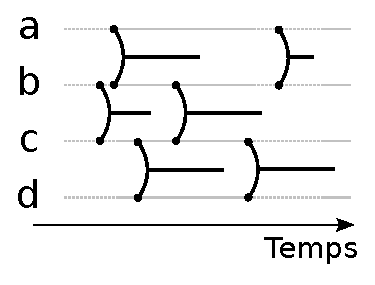
\includegraphics[width=\linewidth]{img/Intro/sous_flots.eps}\hfill
		\caption{Flot de liens initial $L$}
		\label{fig:exemple_sous_flot_init}	
	\end{subfigure}\hspace{0.1\linewidth}
	\begin{subfigure}{0.25\linewidth}
		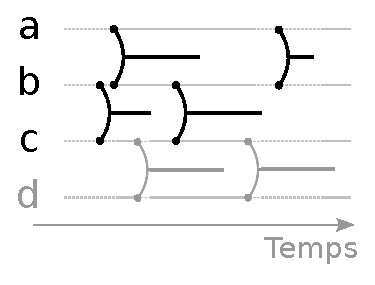
\includegraphics[width=\linewidth]{img/Intro/sous_flots1.eps}\hfill
		\caption{Sous-flot induit par des n\oe{}uds: $L(b)$}	
		\label{fig:exemple_sous_flot1}	
	\end{subfigure}\hspace{0.1\linewidth}
	\begin{subfigure}{0.25\linewidth}
		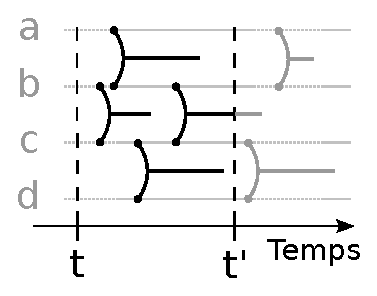
\includegraphics[width=\linewidth]{img/Intro/sous_flots2.eps}\hfill
		\caption{Sous-flot induit par le temps:  $L_{t..t'}$}
		\label{fig:exemple_sous_flot2}	
	\end{subfigure}
	\caption{Exemple de différents sous-flots, (B) et (C), du flot initial en (A). Les liens en noirs sont les liens sélectionnés dans le sous-flot. }
\label{fig:exemple_sous_flot}
\end{figure}
Enfin, il est aussi possible de combiner ces notions.
Par exemple avec $V' \subset V$, $L_{t..t'}(V'\,^2)$ est le sous-flot correspondant aux liens entre les n\oe{}uds de $V'$ sur l'intervalle $[t, t']$.

\bigskip

Un sous-flot induit par un ensemble de paires de n\oe{}uds peut être construit de manière quasiment linéaire en nombre de liens dans le sous-flot.
Pour un ensemble de paires de n\oe{}uds $S= V_1 \times V_2$, il suffit d'itérer sur l'ensemble des liens qui sont reliés aux n\oe{}uds de $V_1$ et de vérifier que l'autre n\oe{}ud du lien appartient à $V_2$. ce qui se fait en $O(\log(|V_2|))$ pour chaque lien.
Le parcours des liens reliés à $V_1$ peut être fait en $O(|L(V_1 \times V)|)$ si chaque n\oe{}ud a la connaissance des liens auxquels il est relié.
Si tel est le cas alors il est possible de construire le sous-flot en $O(|L(V_1\times V)|\log(|V_2|))$.
Il faut tout de fois distinguer le cas où $S= V_1 \times V$ car il n'est alors pas nécessaire de faire la vérification et la complexité est alors $O(|L(V_1\times V)|)$.

Pour l'intervalle de temps, la situation est plus compliquée car il n'est pas facile de connaître l'ensemble des liens existant à un instant donné.
Il est possible de les trier par ordre d'apparition ou de disparition mais il n'y a pas d'ordre total sur la présence des liens.
Pour qu'un lien, $l= (b,e,u,v)$ appartienne au sous-flot temporel sur $[t,t']$, il doit remplir les deux conditions suivantes:
\begin{itemize}
\item \textbf{$b \leq t'$} le lien commence avant la fin de l'intervalle $[t,t']$.
\item \textbf{$e \geq t$} le lien finit après le début de l'intervalle $[t,t']$.
\end{itemize}


Il n'est donc pas nécessaire de considérer les liens ayant un temps de fin inférieur à $t$.
De manière analogue, il n'est pas nécessaire de considérer les liens ayant un temps de début supérieur $t'$.
Cependant ces deux conditions ne peuvent pas être combinées pour restreindre le nombre liens considérés.
Une manière de construire le sous-flot temporel est d'itérer sur tous les liens dans l'ordre temporel d'apparition et d'arrêter le parcours dès qu'un lien a un temps de début supérieur à $t'$.
Il faut cependant tester l'appartenance de chaque lien parcouru.
Il n'est pas possible de restreindre d'avantage le parcours car l'ensemble des liens débutant entre $\alpha$ et $t$ peuvent être dans le sous-flot en respectant la dernière condition.
De manière analogue, il est possible d'itérer sur les liens dans l'ordre inverse de disparition des liens et de s'arrêter dès qu'un lien a un temps de fin inférieur à $t$.


Dans le pire des cas, ces méthodes sont donc linéaires sur le nombre total de liens dans le flot et non dans le sous-flot comme précédemment.
Il n'y a alors que deux optimisations possibles.
Il est possible de choisir le sens du parcours si les deux ordres sont disponibles.
Si la plus longue durée de liens, $\bar{l}_{max}$, est connue, alors il est possible de commencer la recherche à partir du premier lien respectant $b+\bar{l}_{max} \geq t$.



\section{Degré et densité}
\label{sec:def_densite}
Nous avons défini des outils pour manipuler et extraire des sous-flots d'un flot de liens.
Nous nous intéressons maintenant à étendre quelques notions existantes dans les graphes, en particulier le degré et la densité.


Il est assez trivial de définir le degré temporel d'un n\oe{}ud $u$ de la manière suivante:
\begin{equation}
d(t,u)= |L_t(u)|= \sum_{v \in V} \zeta_{L}(u,v,t).
\end{equation}
Le degré temporel n'est alors pas une valeur comme dans les graphes mais une fonction qui dépend du temps.
Comme les liens apparaissent et disparaissent de manière instantanée, la fonction de degré est une fonction constante par morceaux.
Un exemple de degré temporel est présenté dans la figure~\ref{fig:exemple_degre}.

\begin{figure}
\centering
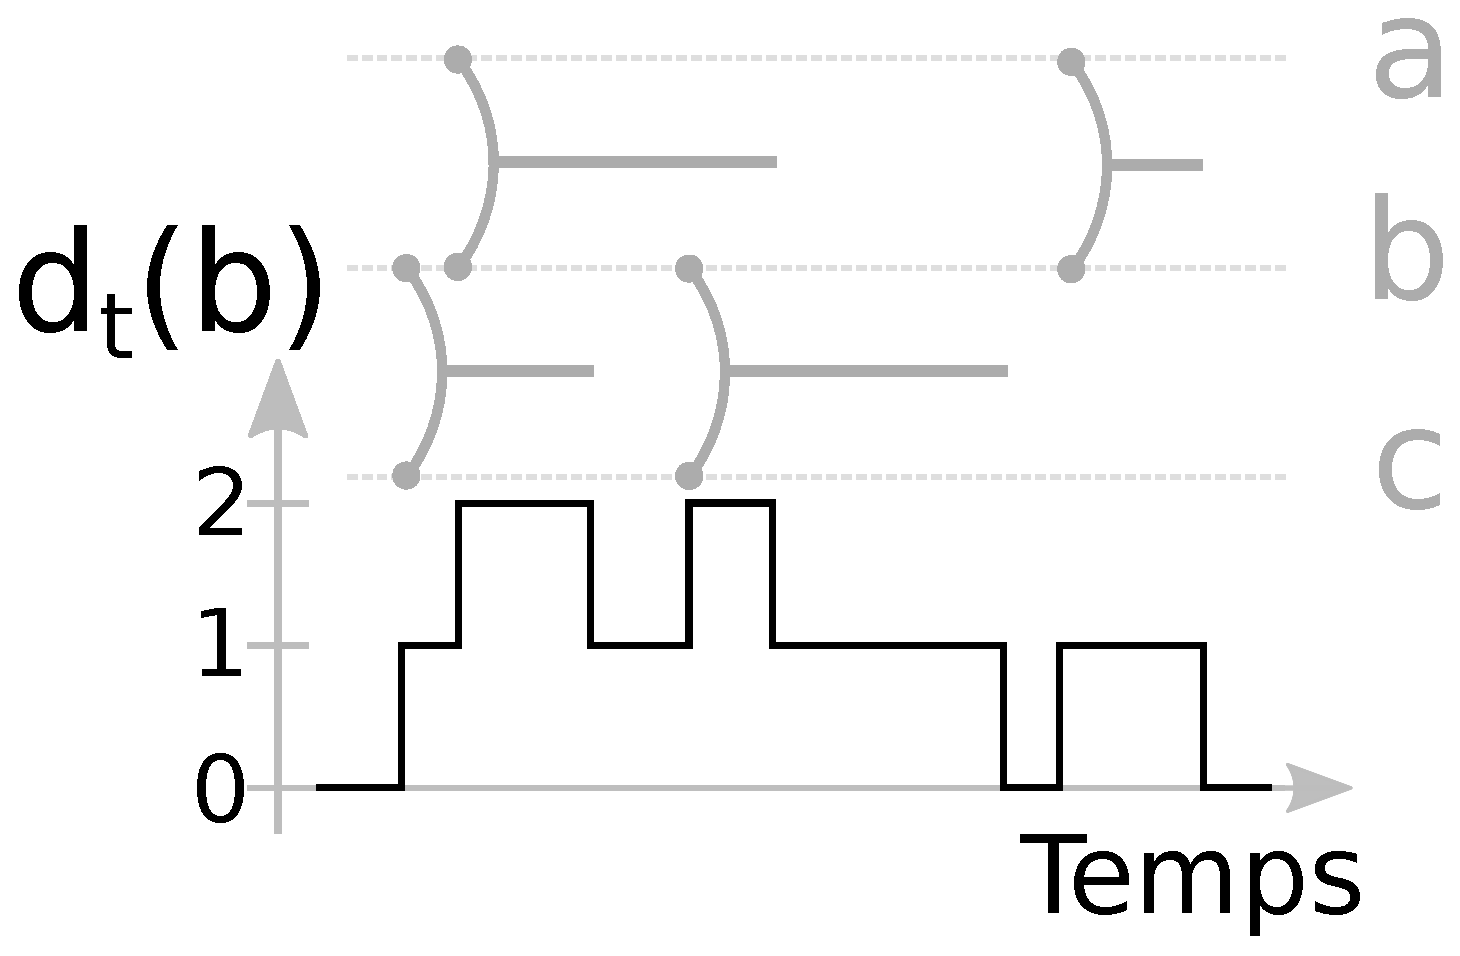
\includegraphics[width=0.35\linewidth]{img/Intro/degre2.eps}
\caption{Degré temporel du n\oe{}ud $b$ dans le flot de liens dans la figure~\ref{fig:exemple_sous_flot_init} qui est également rappelé en grisé dans cette figure.
}
\label{fig:exemple_degre}
\end{figure}

De manière analogue aux graphes, il est également possible de définir le degré temporel d'un ensemble de n\oe{}uds, $d_t(V')$ , ou d'un ensemble de liens, $d_t(E')$:

\begin{equation}
d(t, V') = \sum_{v \in V'} d(t,v) = 2 |L_{t}(V'\times V')|+ |L_{t}(V'\times V \setminus V')|\,,
\end{equation}

\begin{equation}
d(t, E')=2|L_{t}(E')| \,.
\end{equation}

Avec ces définitions, il est aussi possible définir les notions de degré temporel interne, $d_{in}(t,V') = 2 |L_{t}(V'\times V')|$, et externe $d_{out}(t,V')=|L_{t}(V'\times V \setminus V')|$.
Les degrés temporels d'un n\oe{}ud, d'un ensemble de n\oe{}uds ou de liens peuvent se calculer rapidement.
Il faut pour ce faire considérer les liens appartenant au sous-flot induit respectivement par un n\oe{}ud, ensemble de liens ou un ensemble de paires de n\oe{}uds.
Il faut d'abord transformer les liens $(b,e,u,v)$ du sous-flot en une suite de modifications de la forme $(b,+1)$ et $(e,-1)$ ce qui a une complexité en $O(m)$.
Une fois cette liste créée, il suffit d'ordonner ces modifications dans l'ordre temporel, ce qui peut être fait en temps $O(2m\log(2m))$, puis d'itérer sur l'ensemble des modification en sommant au fur et à mesure les apparitions et disparitions de lien, ce qui peut être fait en temps $O(2m)$.
Ainsi, le degré temporel à un instant $t$ est égal à la valeur de la somme des modification à cet instant.
\bigskip

Les degrés sont des fonctions du temps mais il est souvent intéressant de regarder la somme pondérée du degré, que l'on note $D_{t..t'}(u)$, et le degré moyen, que l'on note $d_{t..t'}(u)$, sur un intervalle donné:
\begin{equation}
D_{t..t'}(u)= \int_{t}^{t'}d(t,u) dt  = \sum_{l \in L_{t..t'}(u)}\bar{l} \qquad
d_{t..t'}(u)= \dfrac{D_{t..t'}(u)}{t'-t}\, .
\label{eq:deg_moyen}
\end{equation}

Lorsque cela n'est pas ambigu, nous notons $d_{\alpha..\omega}(u) = d(u)$.
Il est intéressant de noter dans cette formulation que si tous les liens durent tout au long du flot de liens alors le degré dans le graphe agrégé et le degré moyen dans le flot de liens sont égaux, c'est-à-dire  $d_{\alpha..\omega}(u) = d_{G(L)}(u), \forall u \in V$.

\`A partir du degré, il est possible de définir beaucoup de notions différentes et notamment la densité.
Pour rappel, la densité dans un graphe est définie par $\delta(G)=2m/(n(n-1))=d(V)/n(n-1)$ et est égal à la probabilité qu'il existe un lien entre 2 n\oe{}uds pris au hasard.
Si l'on transpose l'idée au formalisme de flot de liens, la densité dans un flot de liens est la probabilité qu'il existe un lien entre 2 n\oe{}uds à un instant donné aléatoire.
Cela se traduit par la formule suivante:
\begin{equation}
\delta(L)= \dfrac{2 \sum_{l \in E}\bar{l}}{n(n-1) (\omega-\alpha)}.
\end{equation}

Cette formulation est équivalente à la densité moyenne des graphes $G(L_t)$:

\begin{equation*}
\dfrac{1}{\omega-\alpha} \int_{\alpha}^{\omega} \delta(G(L_t)) dt=
\dfrac{1}{\omega-\alpha} \int_{\alpha}^{\omega} \dfrac{d(t,V)}{n(n-1)}dt=
 \dfrac{1}{\omega-\alpha} \int_{\alpha}^{\omega} \dfrac{\sum_{u \in V} d(t,u)}{n(n-1)}dt
 \end{equation*}

 \begin{equation*}
= \dfrac{\sum_{u \in V} \int_{\alpha}^{\omega}d(t,u)dt}{n(n-1)(\omega-\alpha)} =
\dfrac{\sum_{u \in V} \sum_{l \in L_(u)} \bar{l}}{n(n-1)(\omega-\alpha)} =
\dfrac{2\sum_{l \in E}\bar{l}}{n(n-1) (\omega-\alpha)} .
\end{equation*}

Pour arriver à ce résultat, nous utilisons la relation entre degré temporel moyen et somme des durées de l'équation~\ref{eq:deg_moyen}.

La notion de densité que nous avons définie est donc cohérente avec notre notion de degré et traduit le même concept que dans les graphes.
Ainsi, la densité dans les flots de liens est aussi comprise entre à $0$ et $1$.
Enfin, cette formulation de densité est une généralisation de la densité proposée par Viard \emph{et al.}~\cite{Viard2014a} qui ne considérait que les liens sans durée.
Les auteurs considèrent l'ajout de temps arbitraire sur chaque lien.
Leur formulation est équivalente à la densité suivante: $\delta( \sigma(\xi(L,\Delta)))$ si l'augmentation de la durée ne se fait pas de manière symétrique.
Un lien est $(t,t,u,v)$ est transformé en un lien $(t-\Delta,t,u,v)$.

Le calcul de la densité d'un flot est linéaire en le nombre de liens car il est dépendant du calcul de $d_{\alpha..\omega}(V)$  qui est fait de manière linéaire.


\begin{table}
	\centering
	\begin{tabular}{|c|c|}
	\hline Symbole & description \\
	\hline $L$ & Flot de liens \\ 
	$T$ & intervalle de temps  \\
	$V$ & ensemble de n\oe{}uds\\
	$E$ & ensemble de liens: $(b,e,u,v)$ \\
	$|L|,|E|$ & nombre de liens dans le flot \\
	$\beta(E)$ & temps d'apparition du premier lien\\
	$\psi(E)$ & temps de disparition du dernier lien\\
	$\xi(L,\Delta)$ & augmentation de la durée de chaque lien de $\Delta$\\
	$\sigma(L)$ & Simplification du flot de liens $L$\\
	$G(L)$ & graphe agrégé de $L$\\
	$L(V_1\times V_2)$ & sous-flot induit par l'ensemble de paires de n\oe{}uds $V_1\times V_2$ \\
	$L_{t..t'}$ & sous-flot induit par l'intervalle $[t,t']$ \\
	$L_{t}$ & sous-flot induit par un instant $t$\\
	$d_t(v)$ & degré de $v$ à l'instant $t$\\
	$d_t(V)$ & somme des degrés des n\oe{}uds dans $V$ à l'instant $t$\\
	$d_{in}(t,V')$ & somme des degrés internes des n\oe{}uds dans $V'$ à l'instant $t$\\
	$d_{t..t'}(v)$ & degré moyen de $v$ sur $[t,t']$\\
	$D_{t..t'}(u)$ & somme pondérée du degré de $v$ sur $[t,t']$\\
	$d(v)$ & degré moyen $v$ sur $T$\\
	$\delta(L)$ & densité du flot\\
%	$\delta_{\Delta}(L)$ & densité du flot où chaque lien dure $\Delta$\\
	\hline
	\end{tabular} 
		\caption{Liste des notations pour les flots de liens}
\end{table}

\bigskip
D'autres notions ont par ailleurs été définies dans les flots de liens  dans la thèse de Tiphaine Viard~\cite{viard2016flots}.

\section{Manipulation concrète des flots de liens}

Nous avons défini formellement quelques notions pour les flots de liens.
Afin de manipuler ces notions simplement, nous avons mis en place une librairie capable de les calculer.
Le but est de fournir une implémentation générale qui soit simple d'accès.
Ainsi, il sera possible à n'importe qui de calculer ces notions.
La démarche, bien que beaucoup plus modeste, est similaire à ce qui est fait pour les graphes avec \emph{networkx}\,\footnote{\url{https://networkx.github.io/}}.

L'implémentation est en \emph{C++} pour la rapidité avec un export en \emph{python} pour faciliter l'utilisation.
Le code de cette implémentation est en ligne\,\footnote{\url{https://bitbucket.org/nGaumont/liblinkstream/}} et la documentation également\,\footnote{\url{https://linkstream.ngaumont.fr/}}.
Il est, par exemple, possible avec la librairie de lire un flot de liens et de calculer la densité moyenne d'un sous-ensemble de n\oe{}uds sur un intervalle arbitraire.
Comme le but de cette librairie est d'être généraliste, l'implémentation n'est pas optimisée pour un calcul spécifique.
Ainsi, il est aisé d'étendre la librairie afin de permettre le calcul de nouvelles notions.
 

Un intérêt de cette implémentation est de permettre, en python, la génération de visualisation\,\footnote{Pour  l'instant, uniquement un export en svg est possible.}, voir le dessin dans la figure~\ref{fig:exemple_Flot_de_liens_lib}.
Parmi les possibilités offertes par la visualisation, il est possible de n'afficher qu'une partie des n\oe{}uds ou de ne garder qu'un sous intervalle de temps.
De plus, il est possible de choisir la couleur des liens de manière manuelle ou en fonction d'une partition de liens.

\begin{figure}
\centering
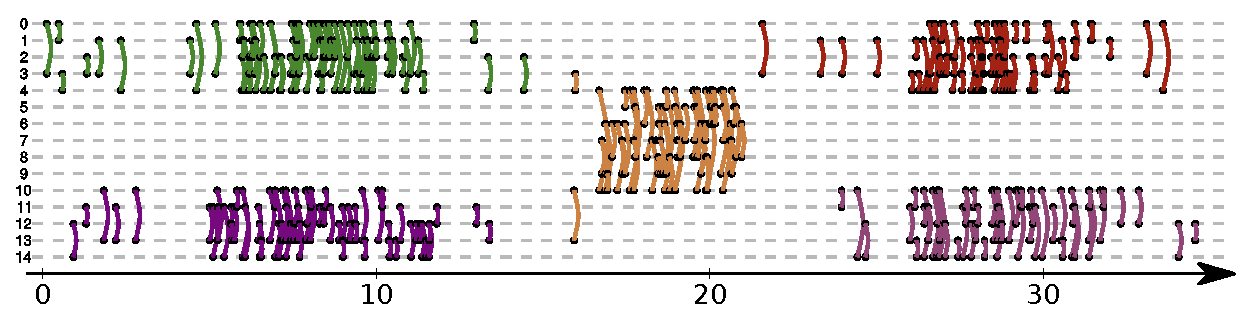
\includegraphics[width=\linewidth]{img/Intro/Dessin_Flot.eps}
\caption{Exemple d'une visualisation d'un flot de liens sans durées entre $15$ n\oe{}ds au cours du temps qui a été généré par notre librairie.
La couleur des liens a été fixée par l'utilisateur de la librairie.
}
\label{fig:exemple_Flot_de_liens_lib}
\end{figure}

La lisibilité de ce genre de visualisation est très dépendante de l'ordre attribué aux n\oe{}uds sur l'axes des ordonnées.
C'est pourquoi avec notre outil, il est également possible de fixer un ordre arbitraire.
Comme il peut être fastidieux d'écrire un ordre, nous avons implémenté un algorithme rudimentaire pour améliorer l'ordonnancement des n\oe{}uds dans la visualisation.
Afin de pouvoir améliorer une visualisation, il est nécessaire de pouvoir quantifier la complexité de la visualisation actuelle.
Empiriquement, on se rend vite compte que ce sont les longs traits verticaux qui rendent la visualisation complexe.
Il faut donc les limiter.

C'est pourquoi nous décidons d'évaluer un ordonnancement par la somme des longueurs des traits représentant les liens.
Avec la fonction d'ordre $Ordre: V \longmapsto \mathbb{N}$, trouver le meilleur ordonnancement se résume à résoudre:

\begin{equation}
 Ordre* = \argmin_{Ordre}  \sum_{(b,e,u,v) \in E} |Ordre(u)- Ordre(v)|
\end{equation}

Malheureusement, trouver l'optimum ne semble pas trivial et il n'est pas envisageable de tester l'ensemble des ordres.
C'est pourquoi nous utilisons un algorithme probabiliste qui teste des permutations aléatoires.
Une permutation est appliquée si elle améliore l'évaluation de la visualisation.
Il s'agit bien sûr d'une première approche qu'il est possible d'améliorer.

Une piste possible est la construction d'un ordre potentiellement proche de l'optimum.
Par exemple, il serait intéressant de trier chaque paire de n\oe{}uds $(u,v)$ en fonction du nombre de liens existants entre $u$ et $v$ puis de construire itérativement un ordre des n\oe{}uds en fonction de l'ordre des paires de n\oe{}uds.




\chapter{Étude de la structure d'un flot de liens}

L'étude de la structure des réseaux est un sujet qui est étudié depuis assez longtemps \REF.
Ces études ont, dans un premier temps, permis de trouver comment caractériser une structure puis, dans un second temps, de proposer des méthodes de détections de ces structures.
La littérature sur l'étude des flots de liens est encore récente et il n'existe que peu d'études \REF\ sur les spécificités des structures dans les flots de liens.

Nous nous intéressons à une archive de courriels publiquement disponibles\footnote{\url{https://lists.debian.org/debian-user/}}.
L'étude de fil de discussions a déjà étudié dans le passé~\cite{Dorat2007} mais cela a été fait en utilisant des méthodes statiquement.
Cette archives l'ensemble des courriels échangés par différent utilisateurs lors de l'utilisation de debian.
Typiquement, une personne ayant un problème lors de l'installation envoie un courriel à la liste afin de demander de l'aide.
Toutes personnes inscrites sur la liste reçoit cette demande et peut y répondre.
Ces données se transposent facilement sous forme de flot de liens car une personne est un n\oe uds et chaque courriel entre deux personnes donne lieu à un lien dans le flot à l'instant où le courriel a été envoyé.
Le message initiant la conversation est ignoré pour éviter les boucles.
L'avantage de ces données de communications est que nous connaissons la discussion dans laquelle a lieu chaque message.
Une discussion est un ensemble de courriels dont tout les messages répondent à un message précédant excepté pour le premier qui a initié la discussion et que nous appelons $racine$.
Ainsi, nous étudions la structure des discussions dans le flot liens représentant les courriels envoyés sur la liste.

Utiliser le formalisme de flot de liens est particulièrement intéressant car cette lite de diffusion existe depuis 1994.
L'aspect temporelle des discussion est donc important.



\section{Prétraitement sur le jeu de données}
Bien que disponible, ce jeu de données nécessite un ensemble de traitement avant de pouvoir exploiter les 724985 courriels que contenait l'archive en janvier 2015.
Tout d'abords, les données ne sont pas sous la forme d'un flot de liens avec la structure des conversations.
Les données sont accessibles via le site internet.
Pour avoir ces informations sous la forme d'un flots de liens, un script d'extraction a été développé \com{URL}.
Lors de l'extraction, 2269 courriels n'ont pas pu être pris en compte car certaines informations étaient manquantes ou mal formées.

Une fois les informations récupérées, il est nécessaire de vérifier leurs cohérences.
Pour chaque courriel, sont connus d'envoie, l'auteur, le destinataire, le courriel auquel il répond et la discussion dans laquelle il apparait.

Un message peut être filtré pour différentes raisons: le courriel apparait avant le message auquel il est censé répondre, le message auquel il réponds n'est pas présent dans l'archive, l'auteur et le destinataire sont la même personne\footnote{Ce cas est relativement rare.}.
Il s'agit de vérifications simple auquel il faut ajouter les vérification de la cohérence de la structure de discussions.
Ainsi, une discussion est retirée du jeu de donnée si il manque la racine, un de ces messages a été retiré précédemment ou si la discussion a débuté trop récemment ou si elle dure trop longtemps.
Les deux dernières conditions permettent d'éviter un biais envers les conversations incomplètes car trop longues ou trop récentes.
La limite pour considérer une discussion trop récente ou trop longue a été fixé à 2 ans en observant la distribution de durées des discussions, voir la figure~\ref{fig:dists_discussion}.

Une fois tout ces messages filtrés, nous obtenons un flot de liens avec 554233 liens entre 34648 personnes pendant presque 19 ans et 116999 discussions.
Mis à part les courriels de début de discussions, ce sont 53753 courriels qui ont été filtrés soit environ $7\%$.

\inline{Parler de la transformation données -> formalismes flot}
\section{Caractéristiques basiques des discussions}

Les caractéristiques les plus basiques des discussions sont le nombre de courriels, le nombre de personnes, le nombre de paires de personnes distincte en interaction direct et leur durée.
Sur la figure~\ref{fig:dists_discussion} sont présentes les distributions cumulatives inverses de ces notions et on remarque qu'elles sont hétérogènes.

\begin{figure}
\centering
	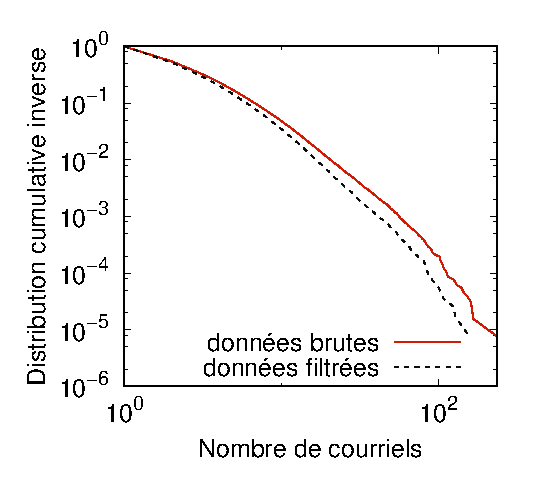
\includegraphics[angle=-90, width=0.49\linewidth]{img/mailing/sizes-ccdf.eps}
	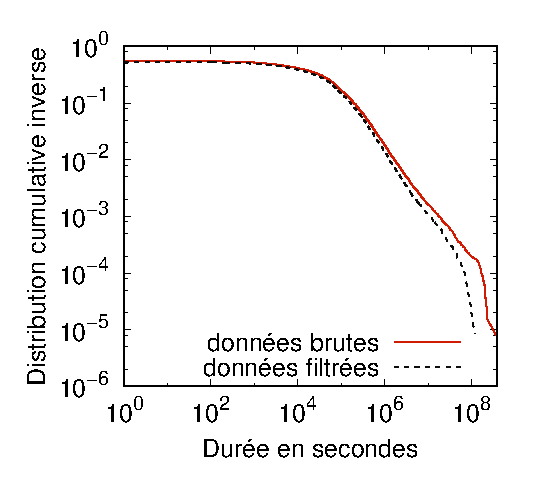
\includegraphics[angle=-90, width=0.49\linewidth]{img/mailing/durations-ccdf.eps}\\
	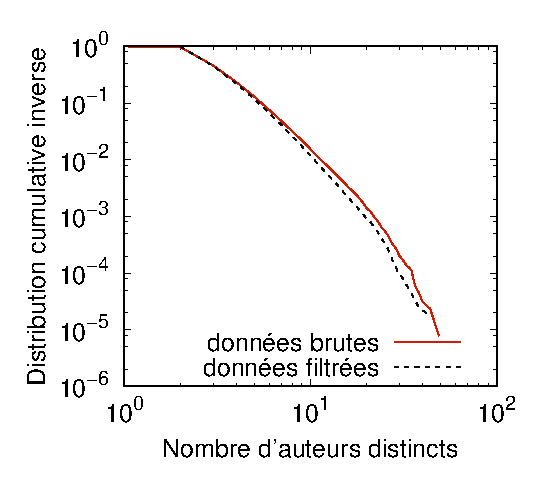
\includegraphics[angle=-90, width=0.49\linewidth]{img/mailing/authors-ccdf.eps}
	\includegraphics[angle=-90, width=0.49\linewidth]{img/mailing/authorpairs-ccdf.eps}
	
	\caption{Distribution cumulative inverse de différentes caractéristiques pour les données brutes (ligne pleine) et filtrées (ligne pointillé). En haut à gauche: nombre de courriels dans une discussion; en haut à droite: durée d'une discussion; en bas à gauche: nombre de personnes dans une discussion; en bas à droite: nombre de paires d'auteurs distinct dans une .}
	\label{fig:dists_discussion}
\end{figure}

La distribution des durées des discussions, mets en avant que la majorité des discussions dure environ une journée (100000 secondes équivaux à moins de 28 heures).
Par ailleurs, on remarque qu'il n'existe que quelques discussions durant plus d'un an.
C'est pourquoi, la limite sur la durée a été fixée à 2 ans.
Enfin, on remarque que les données filtrées ne diffèrent pas qualitativement des données brutes.

Ces premières observations sont nécessaires mais pas suffisante pour comprendre les caractéristiques d'une discussion.
Nous avons également étudié la corrélation de ces différentes notions et une partie d'entre elles sont présentées sur la figure~\ref{fig:corr_discussion}.


\begin{figure}
	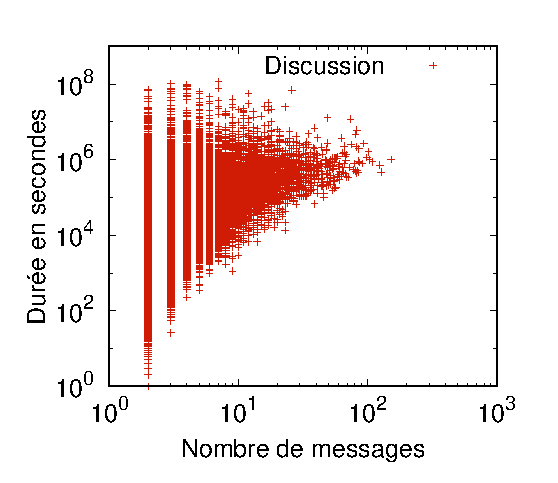
\includegraphics[angle=-90, width=0.49\linewidth]{img/mailing/sizes-durations-corr.eps}
	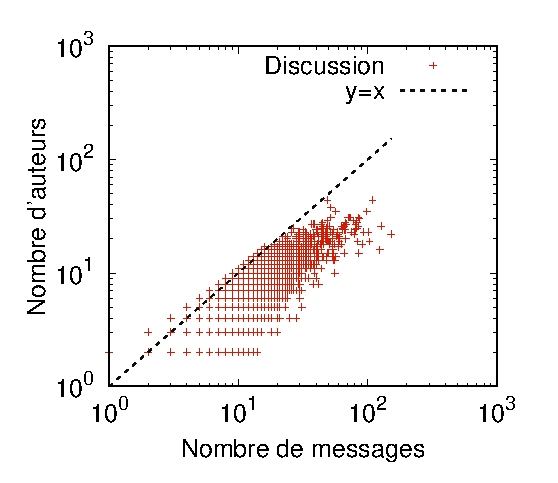
\includegraphics[angle=-90, width=0.49\linewidth]{img/mailing/sizes-authors-corr.eps}
	\caption{Gauche: Corrélations entre le nombre de courriels et la durée d'une discussion. Droite: Corrélation entre le nombre de courriels et le nombre d'auteurs dans une discussion.}
	\label{fig:corr_discussion}
\end{figure}

La corrélation entre la durée et le nombre de courriels, figure de gauche, mets en évidence que plus une discussion est grande en nombre de courriels plus elle dure longtemps ce qui est attendu.
Par contre, on observe également que les petites discussions ont des durées très variables. 
Sur la figure de droite présentant la corrélation entre le nombre de courriels et d'auteurs, on observe également un fait attendu~~\cite{Dorat2007} qui est qu'il y a plus de courriels que d'auteurs. Ainsi lors d'une discussion, c'est un petit nombre de personnes qui partagent beaucoup de messages. 

Enfin, il est intéressant d'observer la dynamique des échanges entre deux personnes.
Soit $\tau(u,v) = (t_{i+1}-t_i)_{i=0..k+1}$ la séquence des temps inter-contacts d'une pair de n\oe uds $u$ et $v$ dans $V$\note{$t_0=\alpha$ et $t_k+1=\omega$}.
Il s'agit du temps écoulé avant que deux personnes se contactent à nouveau.
Sur la figure~\ref{fig:ict_discussion} est représentée la distribution cumulative inverse du temps inter-contacts. 
On remarque que $21\%$ des temps inter-contacts est inférieurs à 30 jours.
Ce chiffre bien que relativement faible est tout de même important car il s'agit d'un fil de discussions ouvert où tout le monde peut participer. 
En particuliers, une personne peut envoyer une demande d'aide à un moment donner et ne plus jamais participer.
\begin{figure}
	\centering
	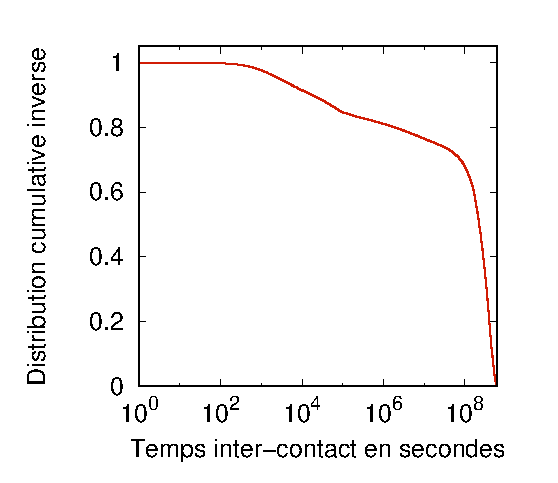
\includegraphics[width=0.49\linewidth]{img/mailing/ict-ccdf.eps}
	\caption{Distribution des temps inter-contacts dans le fil de discussions.}
	\label{fig:ict_discussion}
\end{figure}

\section{Applications de la densité aux discussions}

Jusqu'à maintenant aucune notion intrinsèquement liées aux flot de liens n'a été utilisée pour caractériser les discussion et leur répartition dans le flot de liens.
Le but est d'évaluer si cette structure de flot peut se rapprocher d'une structure communautaire.
Comme dit précédemment, les communautés sont souvent définies comme étant des structure devant être densément connectées.
C'est pourquoi nous nous attachons à étudier la densité des discussions.

Comme ces données se modélisent par un flot de liens ou chaque lien n'a pas de durée, nous étudions la $\Delta$-densité pour différentes valeurs de $\Delta$.
Tout d'abord sur la figure~\ref{fig:dens_fil_discusion} est représenté la $\Delta$-densité globale de tout le flot de liens.
En couvrant un spectre aussi large de $\Delta$, on observe que la $\Delta$-densité est croissante avec $\Delta$ mais surtout on observe bien la convergence de $\Delta$-densité vers la densité du graphe agrégé lorsque $\Delta$ est proche de $\omega - \alpha$.
\inline{Ajout bar horizontal de la densité statique.}

\begin{figure}
	\centering
	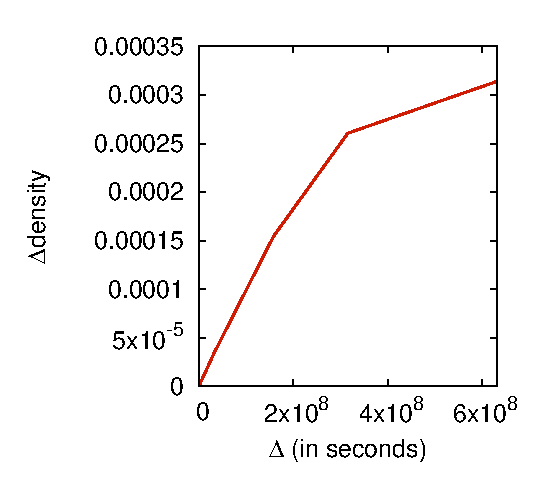
\includegraphics[width=0.48\linewidth]{img/mailing/global_linlin.eps}
	\caption{Évolution de la $\Delta$-densité du flot de liens pour $\Delta$ de $1$ seconde à $20$ ans.}
	\label{fig:dens_fil_discusion}
\end{figure}

La $\Delta$-densité du flot liens, cependant, n'apporte que peu d'informations en elle-même.
Elle est surtout utile pour comparer les valeurs de $\Delta$-densité des sous-flots que sont les discussions.
Ainsi sur la figure~\ref{fig:intra_dens_discussion} est présentée la distribution cumulative inverse de la $\Delta$-densité des discussions pour différentes valeurs de $\Delta$.
On remarque que les différentes valeurs de $\Delta$ ne semblent pas influencer qualitativement la distribution de $\Delta$-densité.
Cette courbe mets surtout en évidence que les discussions sont des structures beaucoup plus denses que le flot.
En effet, la densité médiane des discussions est, selon la valeur de $\Delta$, entre $2.69 \times 10^{-4}$ et $0.28$ alors que le flot a une densité entre $1.05  \times 10^{-10}$ et $3.42 \times 10^{-5}$.
La $\Delta$-densité des discussions est donc en moyenne $10^{5}$ fois plus élevé que celle du flot.
Bien que notable, ce fait est attendu notamment car le flot dure beaucoup plus longtemps et concerne beaucoup plus de n\oe uds.
\begin{figure}
\centering
%\subfloat[Inverse cumulative distribution of intra-threads density.]{
	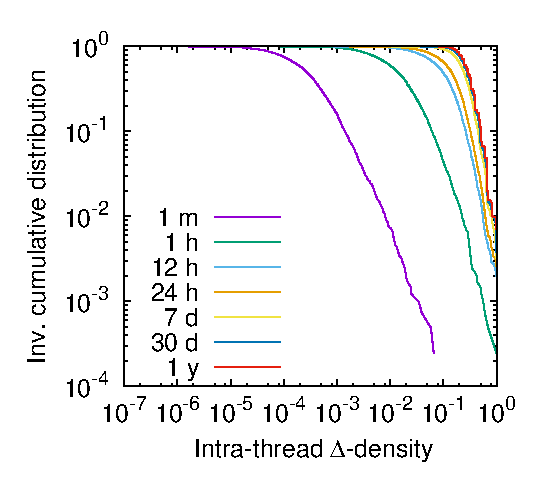
\includegraphics[width=0.48\linewidth]{img/mailing/delta.eps}
%}

\caption{Distribution cumulative inverse de la $\Delta$-densité des discussions pour différentes valeurs de $\Delta$s. Right: Inverse cumulative distributions of values of inter-thread $\Delta$-density for different $\Delta$s.}
\label{fig:intra_dens_discussion}
\end{figure}

Afin d'aller plus loin dans l'étude de cette structure, .


\begin{figure}
\centering
%\subfloat[Inverse cumulative distribution of inter-threads density.]{
	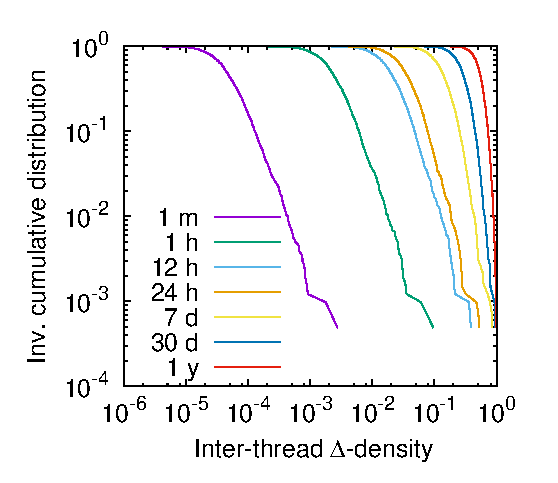
\includegraphics[width=0.48\linewidth]{img/mailing/inter_delta.eps}
%}
\caption{Left: Inverse cumulative distributions of values of intra-thread $\Delta$-density for different $\Delta$s. Right: Inverse cumulative distributions of values of inter-thread $\Delta$-density for different $\Delta$s.}
\label{fig:inter_dens_discussion}
\end{figure}

\section{Détection automatique des discussions?}

Nope

\chapter{Détection de groupes pertinents dans les flots de liens}
\minitoc

\label{groupesDense}
Nous avons vu précédemment qu'il est possible de trouver des groupes de liens dans un flot de liens via l'intermédiaire d'une projection du flot de liens en un graphe statique.
Pour ce faire, nous avons appliqué l'algorithme de Louvain sur la projection pour obtenir une partition des liens en communautés.
Parmi l'ensemble des communautés, il se peut que certaines capturent des structures plus importantes et plus pertinentes que d'autres.
Le but ici est de réussir à extraire parmi ces groupes ceux qui sont pertinents.
En ce sens, nous nous posons la question de la décomposition partielle d'un flot de liens en sous-flots pertinents.
Il s'agit donc d'un problème légèrement différent de la détection de partition car d'une part, certains liens peuvent n'appartenir à aucun groupe et, d'autre part, les groupes doivent être pertinents.

Toute la difficulté pour réussir à trouver les groupes pertinents est de trouver une définition de la pertinence.
La notion de densité, que nous avons utilisée précédemment, est une première approche mais ce n'est pas suffisant.
En effet, il peut exister de grand groupes pertinents mais peu denses et de petits groupes très denses mais peu pertinents.
Il n'est pas possible de faire la différence entre ces deux catégories en utilisant juste la densité.
C'est pourquoi, nous utilisons une notion de voisinage.
Un groupe est alors pertinent s'il est plus dense que son voisinage.
Ainsi, un groupe peu dense peut être pertinent s'il est plus dense que son voisinage.
Comme le but est de pouvoir décrire le flot de liens, nous nous limitons aux groupes ayant une taille supérieure à un minimum donné.
Un exemple de flot avec une décomposition en groupes pertinents est présenté dans la figure~\ref{fig:exemple_groupe_dens}.

Afin de trouver des groupes pertinents, nous procédons de la manière suivante:
\begin{itemize}
\item nous construisons la projection du flot de liens en un graphe statique;
\item nous appliquons sur cette projection un algorithme de détection de communautés afin d'obtenir une partition des liens du flot de liens;
\item nous ne gardons dans la partition que les groupes qui sont considérés comme pertinents, c'est-à-dire ceux qui sont assez gros et qui sont plus denses que leur voisinage.
\end{itemize}

Afin de montrer la pertinence de cette approche, nous l'appliquons sur différents jeux de données et faisons une analyse manuelle de certains groupes trouvés.
Par ailleurs, nous montrons que les groupes que nous détectons ne le sont pas par une méthode statique.

Le chapitre est organisé de la manière suivante.
Dans la section~\ref{sec:groupe_dense_existant}, nous revenons sur les travaux existants qui traitent de sujets similaires.
Puis dans la section~\ref{sec:groupe_dense_method}, nous présentons notre méthode de détection et de validation de groupes pertinents.
Enfin, les jeux de données que nous utilisons sont présentés dans la section~\ref{sec:groupe_dense_result} et les résultats associés dans la section~\ref{sec:groupe_dense_data}.

\begin{figure}
\centering
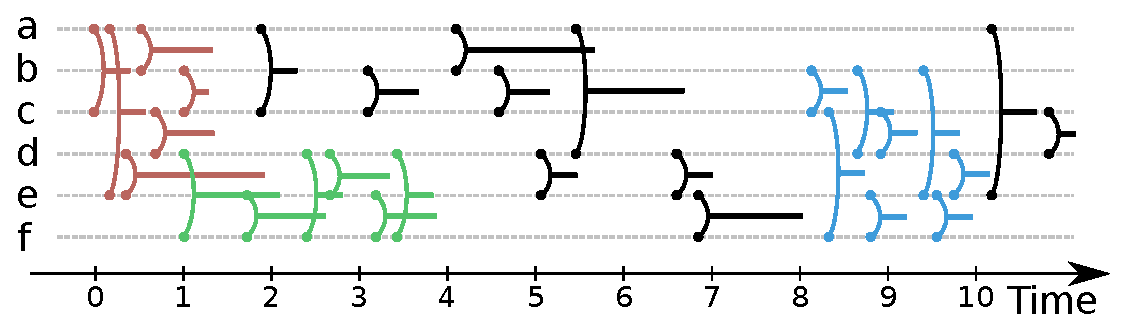
\includegraphics[width=\linewidth]{img/GroupeDense/GroupExample/Zone_dense.eps}
\caption{Exemple de flots de liens avec 3 groupes denses représenté par la couleur des liens (\textcolor{brique}{\textbf{rouge}}, \textcolor{vert_turquoise}{\textbf{vert}} et \textcolor{bleu_window}{\textbf{bleu}}).
}
\label{fig:exemple_groupe_dens}
\end{figure}

\section{Travaux existants}
\label{sec:groupe_dense_existant}

Comme nous l'avons vu dans le chapitre~\ref{chap:etat_art}, il existe assez peu de méthodes cherchant des structures dans un formalisme sans perte d'information.

Mitra~\emph{et al.}~\cite{Mitra2012a} et Speidel~\emph{et al.}~\cite{Speidel2015} ont développé une méthode de détection de communautés mais dans les réseaux diachroniques.
Dans un tel réseau, ce sont les n\oe uds qui ont un \emph{timestamp} et non les liens.
Ce cas de figure s'applique parfaitement aux réseaux de citations car une citation relie bien deux publications apparues à deux dates spécifiques.
Cependant ce genre de situation est particulier et ne peut pas être trivialement représenté par le formalisme de flot de liens.
C'est pourquoi nous ne pouvons utiliser la même méthode. 

Il existe également des méthodes capturant la partie la plus dense d'un réseau.
C'est le cas de Bogdanov~\emph{et al.}~\cite{Bogdanov2011} qui considèrent  un graphe dont la topologie n'évolue pas mais dont les poids des liens changent entre $-1$ et $1$ en fonction du temps.
Ce formalisme est encore une fois très différent de celui de flot de liens.
De plus, la notion de densité utilisée ne tient pas vraiment compte du temps car un groupe de n\oe uds sur un intervalle est évalué par la somme des liens entre ces n\oe uds sur tout l'intervalle.


Epasto~\emph{et. al}~\cite{Epasto2015} capturent le sous-graphe le plus dense dans un graphe temporel.
Ainsi, le temps est bien pris en compte dans le formalisme.
Cependant, la méthode capture le sous-graphe à un instant $t$ tel qu'il ait le degré moyen le plus élevé parmi l'ensemble des sous-graphes sur tous les instants.
La notion de densité est donc statique car elle ne considère que la structure de graphe à un instant.


Enfin les travaux de Rozenshtein~\emph{et. al}~\cite{rozenshtein2014} sont ceux qui se rapprochent le plus de notre méthode.
Leur méthode utilise le formalisme de flots de liens et ne suppose pas de structure de graphe à un instant donné.
Elle capture un groupe de n\oe uds et plusieurs intervalles disjoints de telle sorte que ce groupe de n\oe uds dans le graphe agrégé sur ces intervalles ait le degré moyen le plus élevé.
Plus formellement, un groupe de n\oe uds $V'\subset V$ et un ensemble d'intervalles $\{I_1,..,I_k\} = \mathcal{I} \subset T$ doivent maximiser $\tilde{d}_\mathcal{G}(V')$ où  $\mathcal{G}= \bigcup G(L_t),\,\forall t \in \mathcal{I}$.
Ainsi même si la méthode permet de capturer un groupe de n\oe uds sur des intervalles de temps, elle évalue un candidat sur un graphe agrégé pour appliquer une métrique de graphe.
Le temps n'a donc une influence qu'indirecte sur l'évaluation.
Par ailleurs, leur méthode repose sur plusieurs paramètres qui doivent être fixés \emph{a priori}: le nombre maximum d'intervalles disjoints et la durée cumulée maximum de ces intervalles.
Le premier paramètre permet d'éviter d'utiliser une infinité d'intervalles qui seraient chacun centré sur un lien.
Le second paramètre permet d'éviter de considérer tout le graphe agrégé et ainsi d'imposer la prise en compte du temps.
Ainsi, leur méthode dépend de manière non triviale du choix des paramètres.

\bigskip

Pour résumer, il existe des méthodes cherchant la structure la plus dense dans un contexte dynamique; soit en considérant un graphe temporel soit en considérant un flot de liens.
Cependant, ces méthodes utilisent des métriques de graphes pour évaluer un groupe de n\oe uds.
Le temps n'est donc pas complètement pris en compte dans l'évaluation.
De manière plus importante, ces méthodes évaluent de manière absolue un groupe sans prendre en compte son voisinage.
Enfin, nous capturons plusieurs groupes de liens alors que les autres méthodes capturent un groupe n\oe uds.
Certaines de ces méthodes peuvent être étendues pour capturer les $k$ groupes de n\oe uds les plus denses mais cela se fait au prix de l'ajout d'un paramètre pour contrôler le chevauchement entre deux groupes.


\section{Détection de groupes pertinents}
\label{sec:groupe_dense_method}

Nous avons défini dans le chapitre précédent~\ref{sec:fail_mailing} une projection du flot de liens en un graphe statique.
Dans cette projection, chaque lien du flot est représenté par un n\oe ud.
Deux liens $(b,e,u,v)$ et $(b',e',u',v') \in L$ sont reliés dans le graphe s'ils partagent un n\oe ud et si les intervalles s'intersectent, \emph{i.e.} $\{u,v\} \cap \{u',v'\} \neq \emptyset$ et $[b,e]\cap[b',e'] \neq \emptyset$, voir la figure~\ref{fig:Transformation}.
Sur cette projection, nous appliquons l'algorithme de Louvain pour la détection de communautés.
Les communautés trouvées par l'algorithme sont des groupes potentiellement pertinents et nous les appelons donc groupes candidats.

Tous les groupes candidats ne sont pas forcément pertinents.
Tout d'abord, les groupes d'une partition peuvent avoir des tailles très variées.
En particulier, il peut y avoir beaucoup de très petits groupes de $1$ ou $2$ liens.
Ces groupes ne sont pas pris en compte car nous fixons une taille minimum des groupes fixée \emph{a priori}.

Par ailleurs, l'algorithme de Louvain optimise de manière gloutonne la modularité dans la projection du flot de liens en un graphe statique et non une métrique de flot de liens directement.
C'est pourquoi, certains candidats peuvent être une bonne communauté dans le graphe mais un groupe non pertinent dans le flot de liens.
Cet phénomène est d'autant plus important que la modularité ne prend pas en compte le voisinage d'un groupe.
Par exemple dans la figure~\ref{fig:exemple_groupe_dens}, les liens dans l'intervalle $[4,8]$ forment une composante connexe dans la projection et ils sont considérés comme une communauté par l'algorithme de Louvain.
Or, ces liens ne sont pas un groupe pertinent car ils sont beaucoup moins denses que les liens durant l'intervalle $[0,4]$ ou l'intervalle $[7,11]$.
C'est pourquoi il est nécessaire de filtrer les groupes candidats pour ne garder que les groupes pertinents.




\subsection{Définition des voisinages}
Dans le chapitre~\ref{sec:def_densite}, nous avons défini la densité d'un flot de liens.
Pour un groupe de liens, il faut donc calculer la densité du sous-flot induit par ses liens.
Seulement, la densité en elle même n'est pas un bon critère pour évaluer la pertinence d'un candidat.
En effet, un candidat constitué d'un unique lien a une densité maximale de $1$.
C'est pourquoi il est également nécessaire de tenir compte du voisinage.
Ainsi, plus le candidat a une densité plus importante que son voisinage, plus le candidat est un groupe pertinent.

Il est donc nécessaire de définir une notion de voisinage qui puisse tenir compte à la fois de la structure et du temps.
Pour ce faire, il faut utiliser une autre formulation de la densité pour comprendre quels sont les paramètres qui influent sur la densité.
Jusqu'à maintenant pour un candidat $C_i$, nous considérons la densité du sous-flot induit par ses liens, $\delta(L(C_i))$.
Pour faire apparaître l'influence de la structure et du temps, nous utilisons $\delta(L_{\beta(C_i)..\psi(C_i)}(V(C_i)^2))$ que nous notons, par abus de notation, $\delta(V(C_i),\beta(C_i), \bar{C_i})$ où $\bar{C_i} = \psi(C_i)-\beta(C_i)$.
Il s'agit de la densité des n\oe uds induits par $C_i$ sur la durée du groupe.
Ces deux quantités ne sont pas complètement équivalentes car les deux sous-flots sont différents, en particulier $L(C_i) \subseteq L_{\beta(C_i)..\psi(C_i)}(V(C_i)^2)$.
De cette inclusion découle le fait $\delta(L(C_i)) \leq \delta(V(C_i),\beta(C_i), \bar{C_i})$.
C'est le cas dans l'exemple de la figure~\ref{fig:exemple_groupe_dens} si l'on calcule la densité des liens noirs.
Dans ce cas,  tous les n\oe uds sont induits par ces liens et l'intervalle de temps est égal à $[2,11]$.
Le sous-flot induit par $V$ sur $[2,11]$ comprend l'ensemble des liens noirs mais aussi des liens \textcolor{vert_turquoise}{\textbf{verts}} et \textcolor{bleu_window}{\textbf{bleus}}.


Cependant avec cette formulation, on fait apparaitre 3 dimensions: l'ensemble de n\oe uds, le temps de début et la durée.
Il devient alors aisé de considérer comme voisins les sous-flots qui diffèrent sur une seule dimension: soit le temps de début, soit la durée soit l'ensemble de n\oe uds.
Cette différence entre les voisinages est illustrée dans la figure~\ref{fig:voisinage_groupe}.

\begin{figure}
\centering
	\begin{subfigure}{0.31\textwidth}
		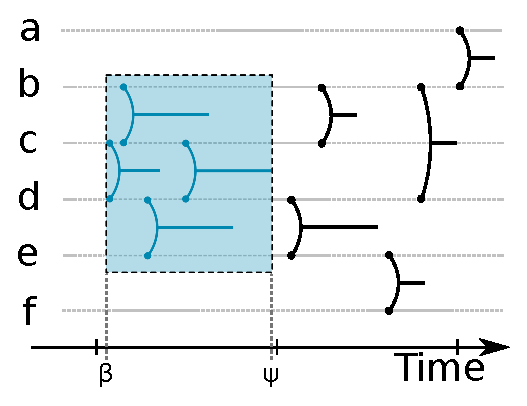
\includegraphics[height=3cm]{img/GroupeDense/GroupExample/Voisinage/Base.eps}
		\caption{Groupe de liens initial}
	\end{subfigure}\hspace*{0.05cm}

	\begin{subfigure}{0.31\textwidth}
		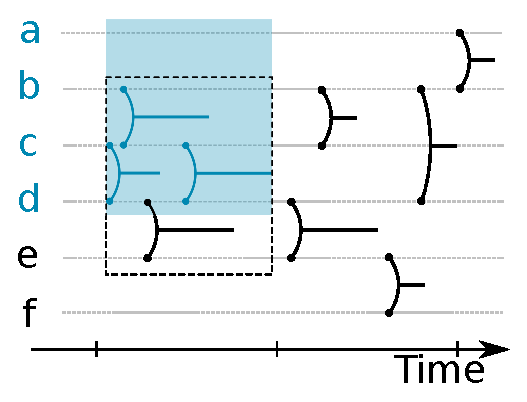
\includegraphics[height=3cm]{img/GroupeDense/GroupExample/Voisinage/Variable_Nodes.eps}
		\caption{Voisinage sur les n\oe uds}
	\end{subfigure}\hspace*{0.02cm}
	\begin{subfigure}{0.31\textwidth}
		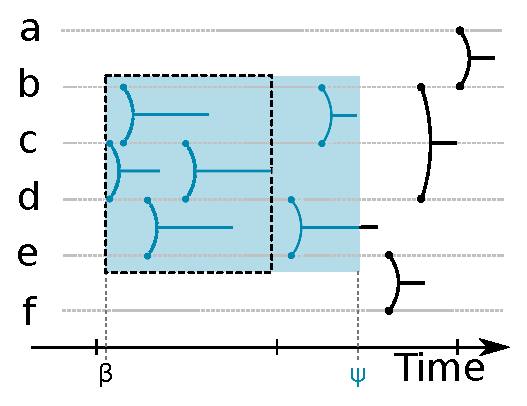
\includegraphics[height=3cm]{img/GroupeDense/GroupExample/Voisinage/Variable_duration.eps}
		\caption{Voisinage sur la durée}
	\end{subfigure}\hspace*{0.02cm}
	\begin{subfigure}{0.31\textwidth}
		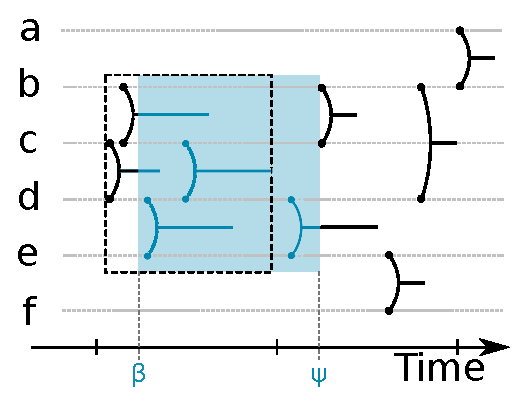
\includegraphics[height=3cm]{img/GroupeDense/GroupExample/Voisinage/Variable_start.eps}
		\caption{Voisinage sur le temps de début}
	\end{subfigure}	
	\caption{Exemple d'un groupe de liens en (A) et de ses différents voisinages en (B), (C) et (D).
	La zone en \textcolor{bleu_transparent}{\textbf{bleu}} est la zone prise en compte lors du calcul de la densité.
	La zone en pointillé représente la zone considérée lors du calcul de la densité du groupe initial.
	}
	\label{fig:voisinage_groupe}
\end{figure}


Pour le voisinage aux n\oe uds, il est impossible de considérer l'ensemble de tous les ensembles de n\oe uds car il est beaucoup trop grand.
De plus, il est probable que ces groupes de n\oe uds ne soient même pas connexes dans le graphe agrégé si le flot de liens est peu dense.
C'est pourquoi, si $V(C_i)$ est constitué de $k$ n\oe uds, nous nous limitons à l'ensemble des groupes de $k$ n\oe uds qui partagent $k-1$ n\oe uds avec $V(C_i)$.
De cette manière, uniquement des groupes de n\oe uds similaires au candidat sont considérés.
Cette comparaison nous semble plus stricte mais plus équitable que celles utilisant l'ensemble des groupes de n\oe uds ou des groupes de n\oe uds pris aléatoirement.
Il serait possible de considérer un nombre moins important de n\oe uds partagés mais nous ne l'avons pas fait à cause de la complexité de calcul.
En effet, il y a déjà $k(|V|-k)$ sous-flots partageant $k-1$ n\oe uds avec un candidat.

Pour le voisinage au temps de début (resp. à la durée), nous considérons toutes les valeurs possibles de temps de début (resp. durée) dans un intervalle donné.
Chacune de ces valeurs donne lieu à un sous-flot induit ayant les mêmes n\oe uds et la même durée (resp. temps de début) que le sous-flot induit par les liens du groupe candidat.
Ensuite, nous calculons la densité de chacun de ces sous-flots voisins.
Pus formellement, l'ensemble des densités des sous-flots voisins se définit de la manière suivante.
Soit $I_{d\acute{e}but}$ et $I_{dur\acute{e}e}$ deux intervalles représentant respectivement les valeurs de temps de début et de durée que nous allons considérer et $C_i$ un groupe de liens.
Les densités des sous-flots dans le voisinage au temps de début sont alors définies par la fonction $\delta(V(C_i),x, \bar{C_i})$, $\forall x \in I_{d\acute{e}but}$.
Les densités des sous-flots dans le voisinage de la durée sont alors définies par la fonction $\delta(V(C_i),\beta(C_i), y)$, $\forall y \in I_{dur\acute{e}e}$.

L'intervalle utilisé pour le voisinage au temps de début est $I_{d\acute{e}but}=[\alpha, \omega-\bar{C_i}]$.
Pour le voisinage à la durée, nous utilisons l'intervalle $I_{dur\acute{e}e}=[0.8\Delta_{min}, 1.2\Delta_{max}]$, où $\Delta_{min}$ (resp. $\Delta_{max}$) est la plus petite (resp. grande) durée de tous les candidats de plus de 10 liens.
Nous utilisons cet intervalle pour deux raisons.
Tout d'abord, il contient l'ensemble des durées acceptables quand nous l'appliquons à nos jeux de données.
Mais surtout, nous avons également testé l'intervalle $[1,\omega-\alpha]$ qui est beaucoup plus grand.
Cela change les résultat de manière quantitative mais pas de manière qualitative.
En effet lorsque la durée considérée est proche de $\omega-\alpha$ alors la densité est très proche de $0$.
Comme ces valeurs sont peu informatives, nous préférons nous limiter à un intervalle de durée plus restreint.
\bigskip

Au final, nous capturons pour chaque voisinage les valeurs de densités des sous-flots voisins.
Pour le voisinage aux n\oe uds, il y a $k(|V|-k)$ valeurs de densité différentes.
Pour le voisinage au temps de début (resp. à la durée), nous avons une fonction de la densité qui dépend du temps de début (resp. de la durée).


\subsection{Définition de l'évaluation}
Nous évaluons chaque groupe candidat en comparant sa densité à celle des sous-flots dans chaque voisinage.
Si un candidat est vraiment pertinent alors il devrait avoir une densité significativement plus élevée que la plupart des sous-flots voisins.
Si les densités des sous-flots voisins suivaient une distribution connue, par exemple une loi normale, alors cela reviendrait à évaluer si la densité du candidat est éloignée de la moyenne en observant le \emph{z-score}.
De par nos observations, les distributions de densité des sous-flots voisins ne suivent pas la même distribution pour différents candidats.
Par exemple, la figure~\ref{fig:distrib_dens} présente des distributions cumulatives de la densité pour le voisinage à la durée pour trois groupes candidats des jeux de donnée Socio Pattern et Rollernet\,\footnote{Ces jeux de données sont présenté dans la section suivante~\ref{sec:groupe_dense_data}.}.
Ces distributions sont très différentes et il n'est pas donc pas justifié d'assumer une unique distribution sous-jacente.
C'est pourquoi nous utilisons les \emph{percentiles} qui représentent la proportion des valeurs de densités qui sont inférieures à la densité du candidat.


\begin{figure}
\centering
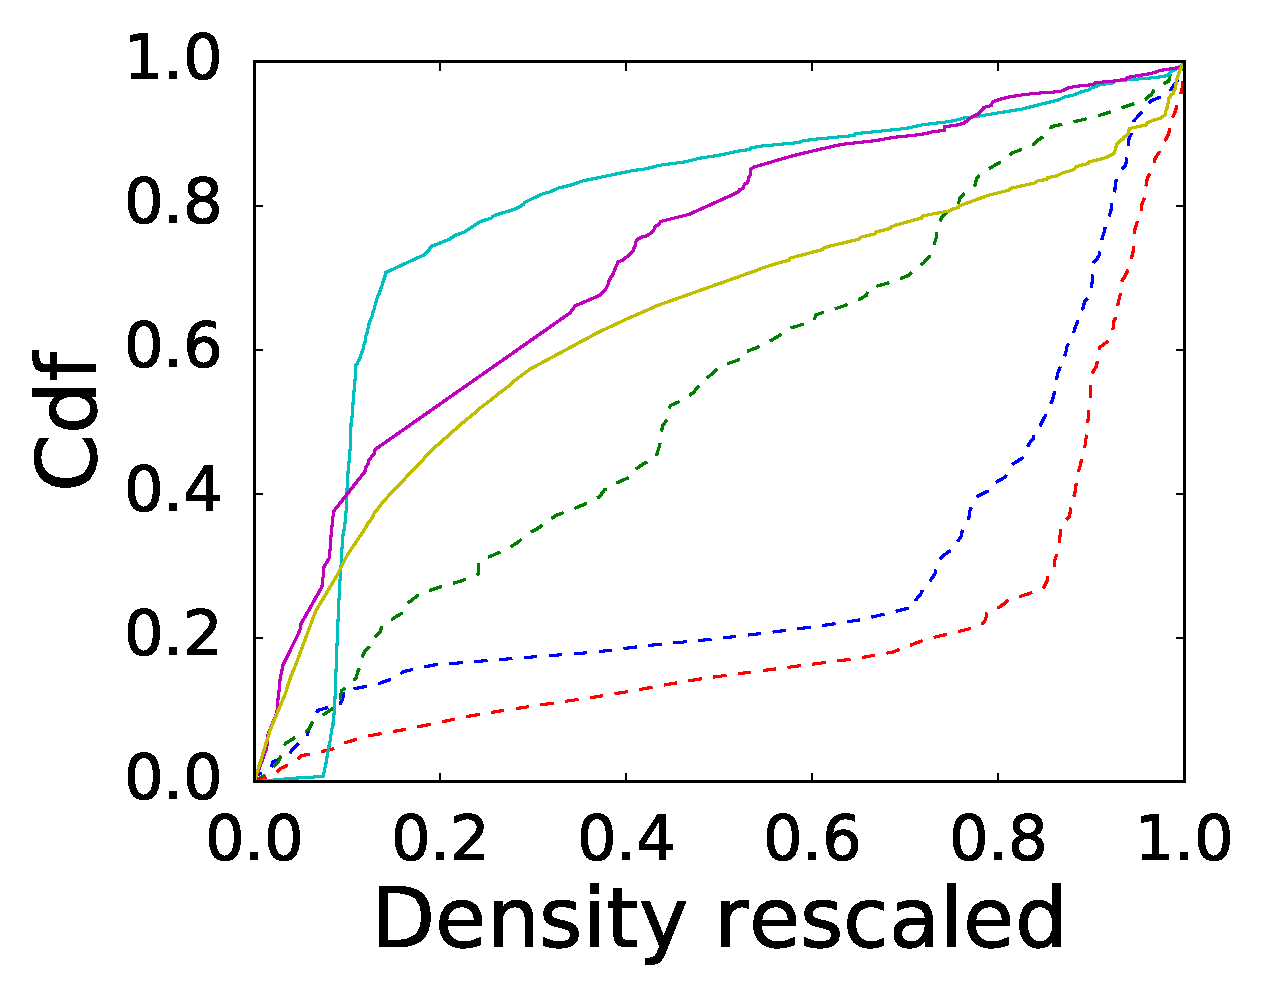
\includegraphics[width=0.3\linewidth]{img/GroupeDense/cdf_density_duration.eps}
\caption{Distributions cumulatives (\emph{cdf}) des valeurs de densité renormalisées des sous-flots voisins dans le voisinages à la durée.
En trait plein (resp. pointillé), trois candidats du jeu de données Rollernet (resp. Socio Pattern).}
\label{fig:distrib_dens}
\end{figure}

Pour le voisinage aux n\oe uds qui est représenté par un ensemble, $S$, de valeurs de densité, le score d'un candidat $C_i$ est:

\begin{equation}
p_{noeud}(C_i)= \dfrac{\sum_{\delta \in S} \mathbf{1}_{\delta \le \delta^*}}{|S|}\,,
\end{equation}
où $\mathbf{1}$ est la fonction indicatrice et $\delta^* =\delta(V(C_i),\beta(C_i), \bar{C_i})$.
Pour les voisinage au temps de début et à la durée qui sont représentés par des fonctions, les scores sont respectivement:

\begin{equation}
p_{d\acute{e}but}(C_i)=\dfrac{1}{\omega-\bar{C_i} - \alpha} \int_{\alpha}^{\omega- \bar{C_i}} \mathbf{1}_{\delta(V(C_i),z,\bar{C_i}) <\delta^*} dz \ ,
\end{equation} 
\begin{equation}
p_{dur\acute{e}e}(C_i)=\dfrac{1}{1.2\Delta_{max} - 0.8\Delta_{min}} \int_{0.8\Delta_{min}}^{1.2\Delta_{max}} \mathbf{1}_{\delta(V(C_i),\beta(C_i),z) <\delta^*} dz \, .
\end{equation}

Un score de $15\%$ pour un voisinage signifie que la densité du candidat est plus faible que $85\%$ des sous-flots dans ce voisinage et que par conséquent le candidat ne devrait pas être considéré comme pertinent.

\bigskip
Pour résumer, un candidat est évalué par un triplet constitué des scores obtenus pour chaque voisinage.
Un candidat est considéré comme pertinent si tous ces scores sont plus élevés que des seuils définis manuellement.
La définition de ces seuils est difficile et dépend des caractéristiques du flot de liens.
C'est pourquoi nous ne les fixons pas \emph{a priori} mais \emph{a posteriori} après avoir examiné la distribution des scores.
Le choix des seuils est décrit plus amplement dans la section~\ref{sec:groupe_dense_result}.

\subsection{Algorithme de calcul des scores}
Nous avons défini formellement les trois voisinages mais il faut encore définir un algorithme efficace pour les calculer.
En effet même s'il n'est pas nécessaire de construire explicitement les sous-flots des voisinages, il est nécessaire de considérer l'ensemble des sous-flots.
Cette nécessité est simple à remplir dans le cas du voisinage aux n\oe uds car il existe un nombre fini de sous-flots voisins.
Pour les voisinages au temps de début et à la durée, il existe une infinité de sous-flots voisins car le temps est continu.

\subsubsection{Voisinage aux n\oe uds}
Pour ce voisinage, il est nécessaire d'analyser des sous-flots durant l'intervalle, $[\beta(C_i),\psi(C_i)]$, mais pour différents ensembles n\oe uds, $V'$.
Il existe plusieurs stratégies possibles pour calculer la densité  de ces sous-flots. 

La première méthode consiste à manipuler chaque sous-flot de manière indépendante et de calculer leur densité.
Pour extraire le sous-flot induit par un ensemble de n\oe uds sur un intervalle de temps,
il est judicieux de d'abord considérer le sous-flot sur les n\oe uds puis d'intégrer le temps  car la construction du sous-flot induit par un ensemble de n\oe uds est plus rapide.
Le calcul de la densité d'un sous-flot induit par un ensemble de n\oe uds $V'$, sur intervalle de temps $[\beta(C_i),\psi(C_i)]$ est alors dépendant du nombre de liens existant entre les n\oe uds de $V'$ avant $\psi(C_i)$ et de la taille de $V'$: $\tilde{C}_{V'}=O(|L_{\alpha..\psi(C_i)}(V'^2)|log(|V'|))$.
$|L_{\alpha..\psi(C_i)}(V'^2)|$ correspond au parcourt de l'ensemble des liens ayant un de leur n\oe uds dans $V'$ et dont il faut vérifier  qu'ils intersectent l'intervalle $[\beta(C_i),\psi(C_i)]$.
Pour chacun de ces liens, il faut également tester que l'autre n\oe ud du lien appartienne également à $V'$ ce qui se fait en $log(|V'|)$.
Pour calculer l'ensemble du voisinage pour un groupe de n\oe uds de taille $k$, il est alors nécessaire de répéter ce processus pour chaque ensemble de n\oe uds ce qui donne une complexité de $O(k(|V|-k) \tilde{C}_{V'})$.
C'est cette méthode que nous avons implémentée.
Elle est d'ailleurs facilement parallélisable.

La deuxième méthode consisterait à tirer parti de la ressemblance des ensembles de n\oe uds dans le voisinage.
La première étape est alors de calculer $d_{t..t'}(V'^2)$, le degré moyen du groupe de n\oe uds initial.
Puis lors de l'évaluation d'un groupe de n\oe uds voisin $V''$, nous savons que $V'$ et $V''$ ne diffèrent que sur un n\oe ud, $v'$ qui est remplacé par $v''$.
Pour calculer la densité de $V''$ sur $[\beta(C_i),\psi(C_i)]$, il suffit de mettre à jour $d_{\beta(C_i)..\psi(C_i)}(V'^2)$ en fonction des liens qui ne sont plus pris en compte et des nouveaux liens pris en compte.
C'est à dire qu'il faut considérer $|L_{\alpha..\psi(C_i)}({v'} \cap V')|$ suppressions de liens et  $|L_{\alpha..\psi(C_i)}({v''} \cap V'')|$ ajouts de liens.
Pour évaluer l'ensemble des voisinages, il suffit de répéter ce processus pour chaque groupe de n\oe uds.
Cette méthode peut également être parallélisée.


\subsubsection{Voisinage à la durée}
Pour le voisinage à la durée, l'ensemble de n\oe uds est fixe et il faut de manière continue augmenter la durée du sous-flot voisin.
Pour réussir à faire cela, il est nécessaire de se baser encore une fois sur le degré temporel de l'ensemble de n\oe uds en question.

La densité dépend d'une part de la somme des degrés du groupe candidat, $D_{\beta(C_i)..\psi(C_i)}(V')$, et d'autre part de la la durée de l'intervalle.
Comme les degrés temporels sont des fonctions constantes par morceaux, la somme des degrés, qui est l'intégrale des degrés, est une fonction linéaire par morceaux dont les points de changement sont les instants où un lien apparaît ou disparaît.
C'est pourquoi, il est possible de définir la densité en fonction de la durée par une fonction par morceaux, voir l'exemple dans la figure~\ref{fig:calcul_var_dure}.
L'idée est de mettre à jour la somme des degrés en fonction de l'apparition et disparition des liens tout en tenant compte de la durée du sous-flot qui augmente linéairement.
La complexité est donc $O(|L_{\beta(C_i)..\beta(C_i)+\Delta_{max}}(V'^2)|)$ si le degré de temporel du groupe est connu.

\begin{figure}
\centering
	\begin{subfigure}{0.4\textwidth}
		\centering
		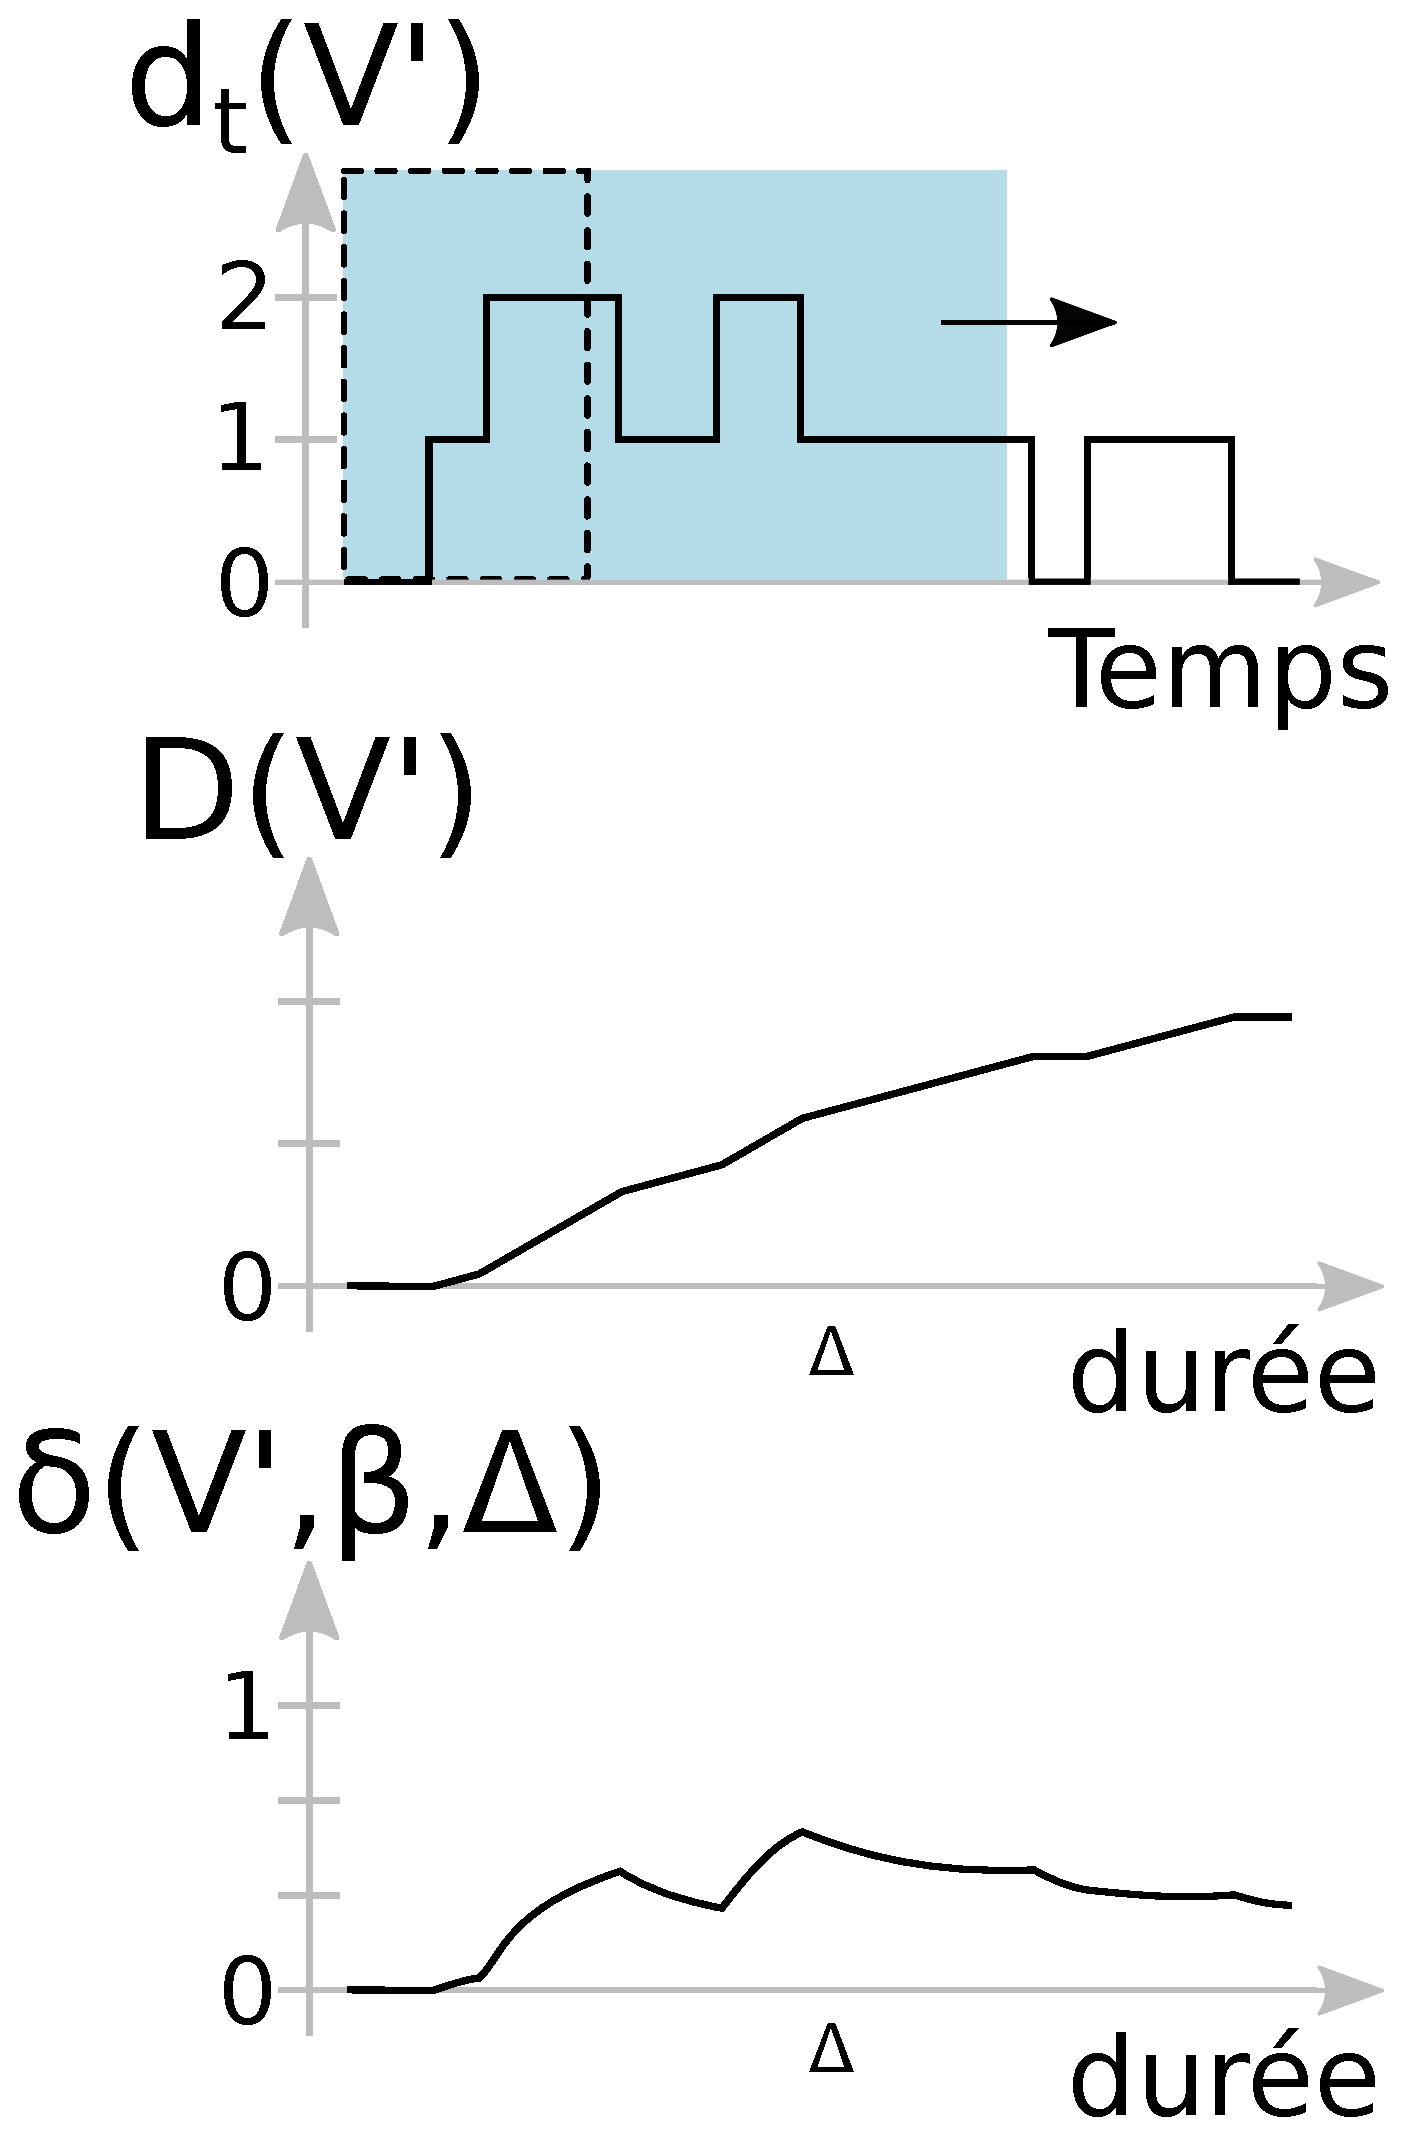
\includegraphics[width=0.8\linewidth]{img/GroupeDense/duration.eps}
		\caption{Voisinage à la durée}
		\label{fig:calcul_var_dure}
	\end{subfigure}\hspace*{0.05\textwidth}
	\begin{subfigure}{0.4\textwidth}
		\centering
		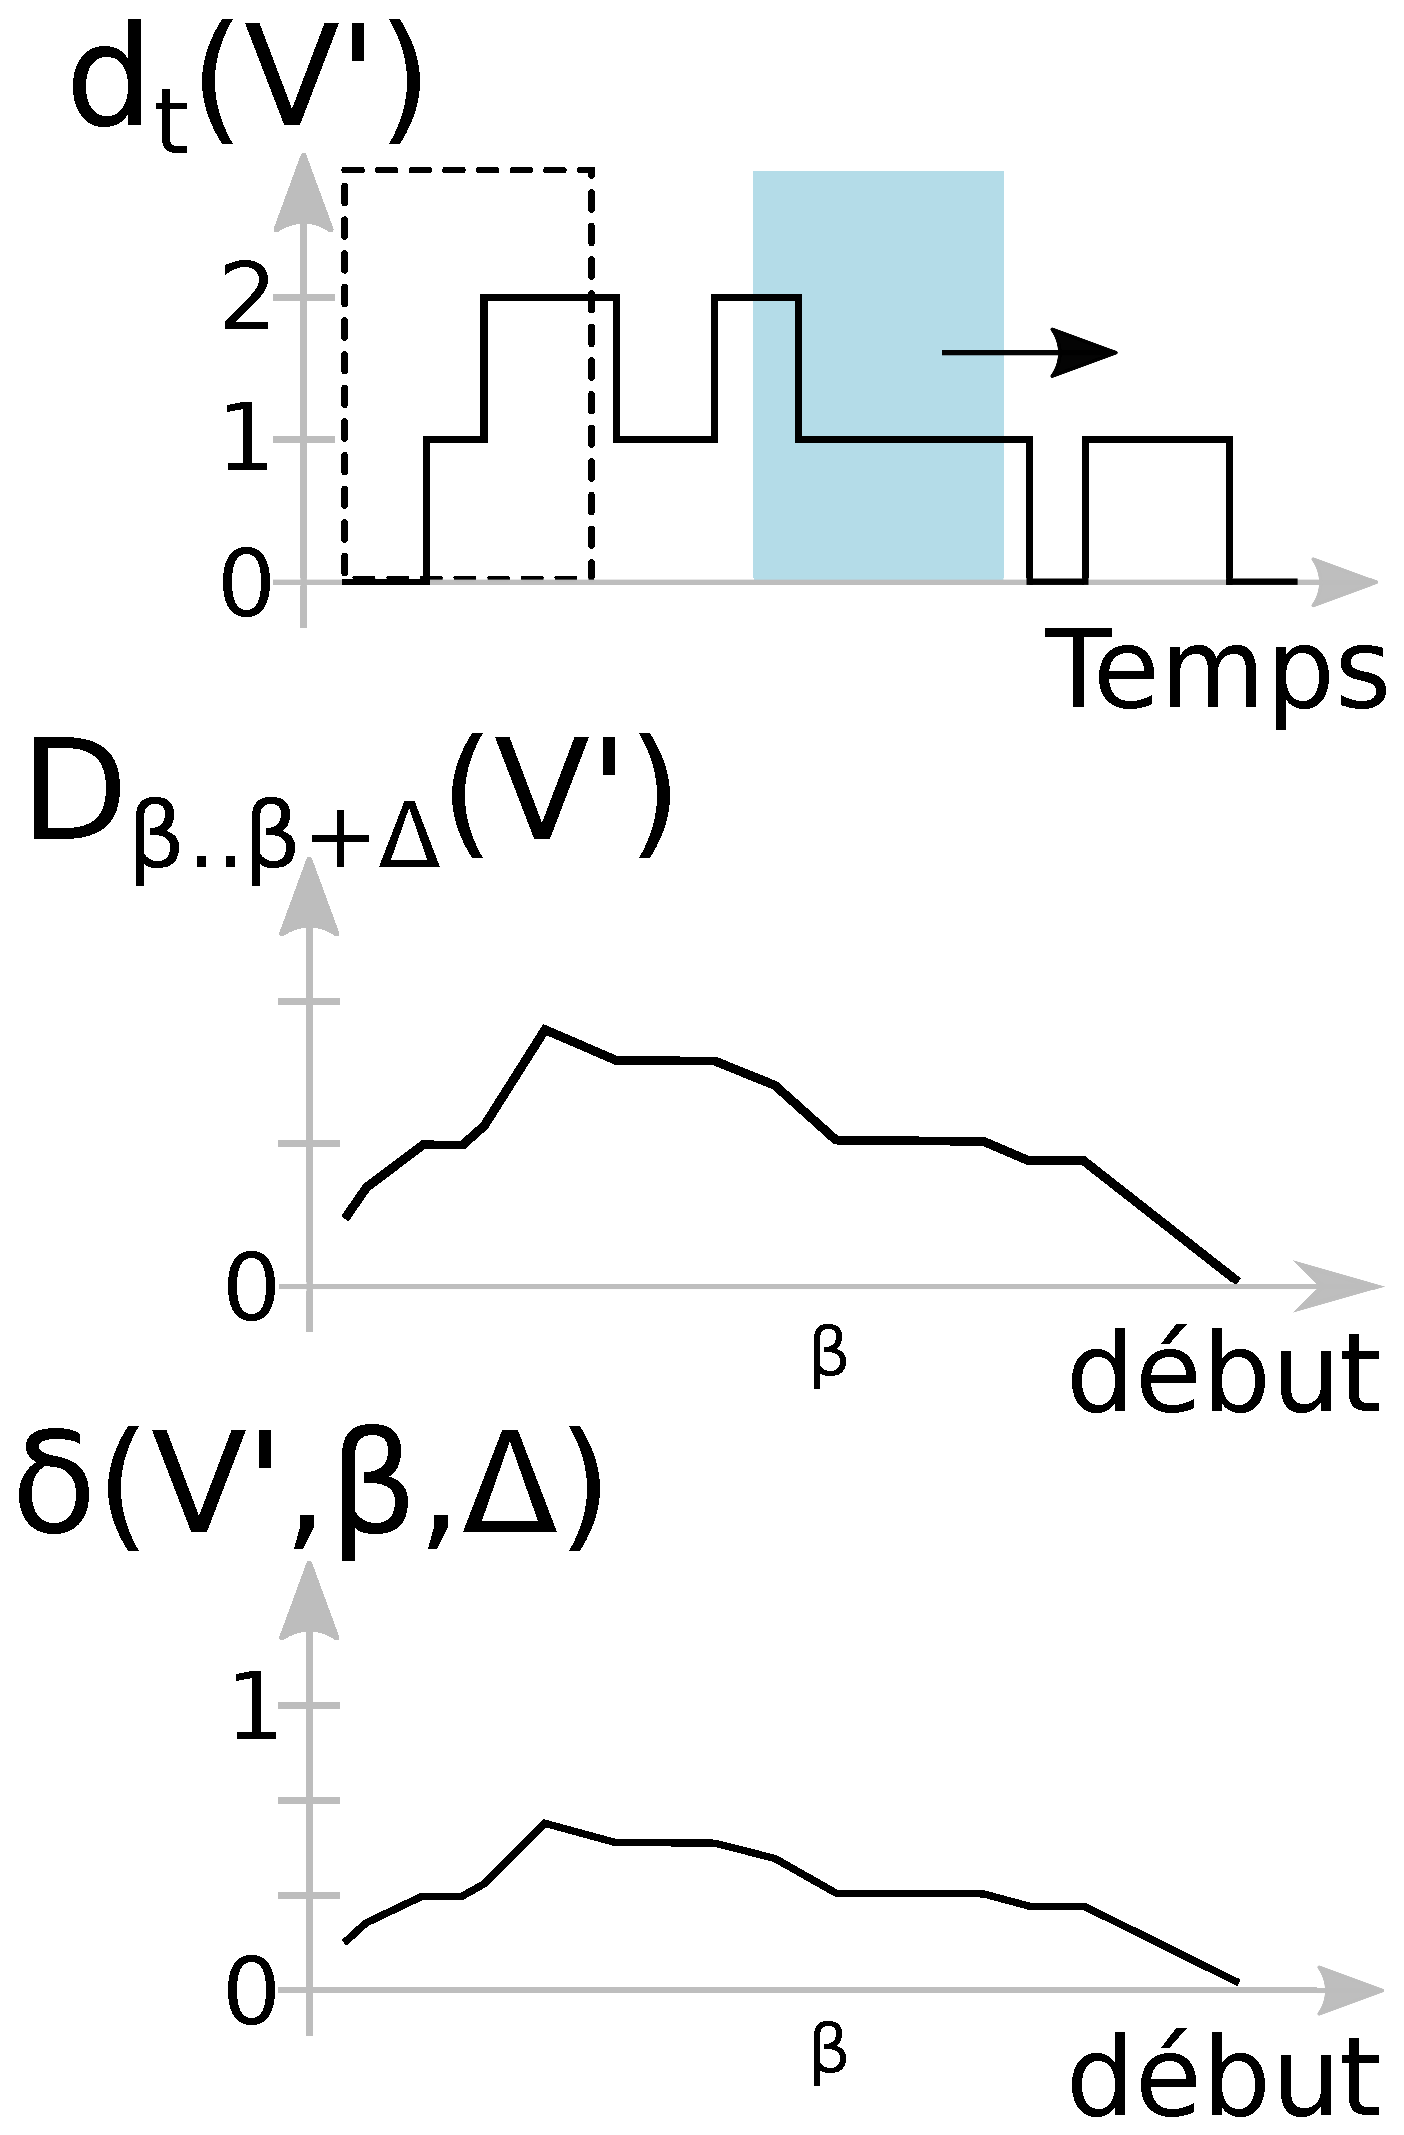
\includegraphics[width=0.8\linewidth]{img/GroupeDense/start_time.eps}
		\caption{Voisinage au temps de début}
		\label{fig:calcul_var_debut}
	\end{subfigure}\hspace*{0.05cm}

	\caption{Calcul du voisinage à la durée en (A) et au temps de début en (B) pour un groupe ayant un degré temporel donné. Le groupe de liens considéré est le même que celui dans la figure~\ref{fig:exemple_degre}.}
	\label{fig:calcul_var_dure_debut.}
\end{figure}

\subsubsection{Voisinage au temps de début}
Pour le voisinage au temps début, l'approche est similaire.
Il faut mettre à jour la somme des degrés.
La principale différence est que les deux bornes de l'intervalle changent, alors que dans le voisinage à la durée seule la borne maximum est modifiée.
Le parcours est donc un peu plus complexe pour calculer $D_{t..t'}(V')$.
Cependant la durée de l'intervalle est fixe, c'est pourquoi il existe une unique bijection entre la somme des degrés et la densité qui est $\delta(V',\beta, \Delta)= \dfrac{D_{\beta..\beta+\Delta}(V')}{|V'|(|V|-1)}$.
Ainsi, la densité en fonction du temps de début est aussi une fonction linéaire par morceaux.

Voir l'exemple dans la figure~\ref{fig:calcul_var_debut}.
La complexité est donc $O(|L_{\alpha..\omega-\Delta}(V'^2)|)$ où $\Delta$ est la durée du groupe.


\section{Jeux de données}
\label{sec:groupe_dense_data}
Nous appliquons notre méthode sur quatre jeux de données différents.
La table~\ref{tab:data_spec_groupe_dense} liste le nombre de n\oe uds, le nombre de liens et la durée de chaque jeu de données.

\begin{table}
\centering
% table caption is above the table

% For LaTeX tables use
\begin{tabular}{|c|c|c|c|}
\hline  \rule[-1ex]{0pt}{3.5ex}
Datasets & $|V|$ & $|E|$ & $\omega - \alpha$  \\
\hline
Socio Pattern & 180 & 19774 & 9 jours \\
Rollernet & 62 & 15803 &  3 heures\\
Reality Mining & 94 & 44975 & 9 mois\\
Babouins & 28 & 95616 & 14 jours\\
\hline
\end{tabular}
\caption{nombre de n\oe uds $|V|$, nombre de liens $|E|$ et durée de chaque jeu de données.}
\label{tab:data_spec_groupe_dense} 
\end{table}

\begin{description}
\item[Socio Pattern~\cite{Fournet2014}]\footnote{\url{http://www.sociopatterns.org}} contient le réseau dynamique d'étudiants d'une école préparatoire à Marseille en 2012. Durant l'expérience, $180$ étudiants de $5$ classes ont porté pendant $9$ jours des capteurs de proximité.
Ainsi, il est possible de savoir quand deux étudiants interagissent. 
Dans ce jeu de données, la classe de chaque étudiant est connue.\\

\item[Rollernet~\cite{Tournoux2009}] a été collecté durant une randonnée roller ayant eu lieu en 2006 à Paris.
Il s'agit d'un événement ayant regroupé $2500$ participants.
Parmi eux, $62$ étaient équipés d'appareils \emph{bluetooth} qui enregistrent l'ensemble des appareils \emph{bluetooth} à portée de communication.
Nous nous limitons uniquement aux contacts ayant eu lieu entre les $62$ personnes portant un capteur.
Des méta-données sont également associées à ces données et notamment le rôle de chaque personne, \emph{e.g.} membre de l'organisation à l'avant du peloton ou membre d'une association de roller.\\

\item[Reality Mining~\cite{Eagle2009}] représente le réseau d'interactions entre $94$ personnes du \emph{MIT Media Laboratory} entre septembre 2004 et juin 2005.
Parmi les $94$ participants, $68$ évoluent dans le même bâtiment (90\% étudiants, 10\% employés) alors que le reste sont des étudiants de l'école de commerce de l'université.
Ce jeu de données a été récolté grâce à des téléphones \emph{bluetooth} prêtés aux étudiants.\\

\item[Babouins~\cite{Crofoot2015,Strandburg-Peshkin2015}] contient la position \emph{GPS} de $28$ babouins (\emph{Papio anubis}) dans le centre de recherche Mpala au Kenya.
Ces $28$ babouins représentent $80\%$ d'une troupe.
Chaque babouin est équipé d'un collier muni d'un capteur \emph{GPS} qui enregistre la position du babouin toutes les secondes.
Nous transformons ces données en un flot de liens en créant un lien entre deux babouins s'ils sont à moins de 1 mètre 50 durant les dernières 10 secondes pour lisser les potentielles imprécisions du \emph{GPS}.
Le code est disponible en ligne\,\footnote{https://bitbucket.org/nGaumont/baboonstreamextractor} et est écrit en \emph{rust}.
\end{description}

Même si ces jeux de données sont des réseaux d'interactions face-à-face, ils sont différents dans leur dynamique.
Par exemple, le jeu de données Rollernet a environ le même nombre de liens que celui de Socio Pattern alors qu'il ne dure que trois heures contre 9 jours pour Socio Pattern.
Enfin, nous n'utilisons pas le jeu de données de courriels utilisé précédemment car notre méthode nécessite un flot de liens avec durées.
Nous pourrions utiliser le flot de liens avec des durées ajoutées artificiellement mais elles ne correspondent à aucune réalité.



\section{Application}
\label{sec:groupe_dense_result}

Pour chaque jeu de données, nous appliquons notre méthode pour capturer les groupes d'interactions pertinents.
Comme présenté dans la section~\ref{sec:groupe_dense_method}, la première étape est de trouver une partition, $\mathcal{C}$, des liens via la méthode de Louvain sur une projection du flot de liens en un graphe statique.
Quelques statistiques obtenues pour chaque partition sont listées dans la table~\ref{tab:partition_spec_gd}, notamment les nombres de n\oe uds et de liens médians.
La première chose qui est frappante est qu'il existe énormément de très petits groupes.
On remarque également que seul le jeu de données Rollernet se distingue des autres en ayant des groupes plus gros.
Cette différence est probablement due au flot de liens qui contient beaucoup de liens pour une durée de seulement trois heures.

\begin{table}
\centering
\begin{tabular}{|c|c|c|c|}
\hline \rule[-1ex]{0pt}{3.5ex}
Jeux de données & $|\mathcal{C}|$ & $\langle|V|\rangle$  & $\langle|L|\rangle$ \\
\hline
Socio Pattern & 12532 (155) & 2 (9) & 1 (15) \\
Rollernet& 559 (75) & 2 (31) & 1 (194) \\
Reality Mining & 5737 (474) & 2 (12) & 1 (36) \\
Babouin & 37671 (1249)  &  2 (7)  & 1 (16) \\
\hline
\end{tabular}
\caption{$|\mathcal{C}|$: nombre de groupes dans la partition, $\langle|V|\rangle$ médiane du nombre de n\oe uds dans un groupe, $\langle|L|\rangle$ médiane du nombre de liens dans un groupe.
Les valeurs en parenthèses correspondent à la valeur quand uniquement les groupes d'au moins $10$ liens sont pris en compte.}
\label{tab:partition_spec_gd}       % Give a unique label
\end{table}


Afin d'avoir une vision plus précise, nous présentons dans la figure~\ref{fig:distri_group_SP} les distributions cumulatives inverses du nombre de n\oe uds, du nombre de liens, de la durée et de la densité des groupes candidats dans le jeu de données Socio Pattern.
Les distributions sont toutes hétérogènes sauf pour la densité.
Les irrégularités dans la distribution de la densité sont dues aux petits candidats; typiquement un groupe de 2 liens entre 3 n\oe uds a une densité de $0.33$ et un groupe avec un seul lien\,\footnote{Ils représentent $83\%$ de tous les candidats.} a une densité de 1.
Les distributions pour les autres jeux de données sont en appendice pages \pageref{fig:distri_group_rollernet} à \pageref{fig:distri_group_RM} dans les figures~\ref{fig:distri_group_rollernet},\ref{fig:distri_group_baboon} et \ref{fig:distri_group_RM}
Pour ces jeux de données, les distributions du nombre de liens, du nombre de n\oe uds et de la durée sont également hétérogènes mais les distributions de densité sont légèrement moins irrégulières.

\groupcharac{Sociopattern}{Socio Pattern}{SP}{}

Comme les très petits groupes de liens ont un intérêt limité pour décrire un flot de liens, nous commençons par écarter les groupes ayant moins de 10 liens.
Même si cela filtre énormément de groupes, il reste tout de même beaucoup de groupes dont il faut encore évaluer la pertinence.

%\groupcharac{RollernetLim}{Rollernet}{rollernet}
%\groupsPerNode{RollernetLim}{Rollernet}{rollernet}
%\percentile{RollernetLim}{Rollernet}{rollernet}
%\groupcharacFilter{RollernetLim}{Rollernet}{rollernet}



\subsection{Évaluation des groupes candidats}

Pour séparer les groupes qui sont pertinents des autres, nous utilisons des seuils.
Un candidat est ensuite considéré comme pertinent si ses scores sont au dessus des seuils choisis.
Baisser les valeurs des seuils entraîne la capture de plus de groupes mais cela ne change ni les groupes candidats ni leurs scores.
Ainsi, si un groupe est considéré comme pertinent pour un seuil donné alors il le sera également pour tout autre seuil inférieur.
C'est pourquoi, nous fixons les seuils après avoir étudié les distributions cumulatives inverses de score pour chaque voisinage.
Ces distributions sont représentées pour le jeu de données Socio Pattern dans la figure~\ref{fig:dit_SP}.
Pour ce jeu de données, les scores sont très élevés, c'est-à-dire proches de $1$, quel que soit le voisinage considéré.
On remarque également que les distributions cumulatives inverses chutent toutes à partir d'une certaine valeur de score, que nous utilisons comme seuil.

\percentile{Sociopattern}{Socio Pattern}{SP}{}

Nous utilisons pour le vosinage au temps de début, à la durée et aux n\oe uds les valeurs de seuils suivantes: $0.998$, $0.85$ et $0.98$.
Pour les autres jeux de données, les distributions de scores sont présentées en appendice page \pageref{fig:dit_rollernet} à \pageref{fig:dit_RM} dans les figures~\ref{fig:dit_rollernet},\ref{fig:dit_baboon} et \ref{fig:dit_RM}.
Elles sont similaires à celles obtenues pour Socio Pattern mis à part pour le jeu de données Rollernet dont les scores sont plus faibles.
Cette différence est sûrement due à la structure plus dense du flot de liens dans le cas de Rollernet.
Enfin, la table~\ref{tab:thresholds} liste les seuils utilisés pour chaque jeu de données.
\begin{table}
\centering
\begin{tabular}{|c|c|c|c|c|}
\hline \rule[-1ex]{0pt}{3.5ex}
Jeux de données & $p_{noeuds}$ & $p_{d\acute{e}but}$  & $p_{dure\acute{e}e}$  \\
\hline
Socio Pattern & 0.98 & 0.998 & 0.85 \\
Rollernet& 0.9 & 0.7 & 0.6 \\
Reality Mining & 0.97  & 0.98 & 0.8 \\
Babouin & 0.95  &  0.99  & 0.85 \\
\hline
\end{tabular}
\caption{$p_{noeuds}$, $p_{d\acute{e}but}$ et  $p_{dur\acute{e}e}$: seuils utilités pour chaque voisinage.}
\label{tab:thresholds}       % Give a unique label
\end{table}

Un candidat est écarté si un de ses scores est en dessous du seuil correspondant. 
C'est pourquoi il est important d'analyser par quels voisinages sont filtrés les groupes.
Les corrélations entre chaque voisinage sont présentées pour le jeu de données Socio Pattern dans la figure~\ref{fig:correlation_SP}.
Les trois voisinages filtrent des candidats différents.
Ils ne sont donc pas redondants.
Même si un score élevé dans un voisinage est souvent corrélé avec un score élevé dans les autres, il arrive qu'un candidat ait un score parfait dans un voisinage et un score très faible dans les autres.
Cette situation se matérialise dans la figure~\ref{fig:correlation_SP} par des groupes situés en haut à gauche ou en bas à droite.
Les corrélations entre chaque voisinage pour les autres jeux de données sont présentées en appendice pages \pageref{fig:correlation_rollernet} à \pageref{fig:correlation_RM} dans les figures~\ref{fig:correlation_rollernet},\ref{fig:correlation_baboon} et \ref{fig:correlation_RM}.


\correlation{Sociopattern}{Socio Pattern}{SP}{}

\bigskip

Afin d'illustrer les scores et les groupes pertinents, nous présentons maintenant une analyse manuelle pour deux candidats extraits des jeux de données Socio Pattern et Rollernet.
Nous avons choisi ces jeux de données pour une analyse manuelle car des méta-données sont également associées, ce qui aide pour la validation des résultats.

\subsubsection{Étude manuelle d'un groupe de Socio Pattern}
Dans les données Socio Pattern, la classe de chaque participant est connue et nous savons également quand commencent les premiers cours et quand ont lieu les pauses.
Le groupe que nous considérons contient $50$ liens entre $17$ n\oe uds et dure environ $15$ minutes, ce qui en fait un des plus gros groupes trouvés.
Comme ce groupe commence à 7h44 le deuxième lundi de la capture, il précède le premier cours de la journée qui a lieu à 8h.
De plus parmi les élèves participants à ce groupe, $16$ font partie de la même classe.
C'est pourquoi il est fort probable que ce groupe corresponde à un regroupement d'élèves avant le premier cours.

Cette analyse est une première étape mais elle ne suffit pas.
En effet, il est possible que ce regroupement ait en réalité concerné d'autres n\oe uds, duré plus longtemps ou même commencé à un autre instant.
C'est pourquoi nous avons développé les notions de voisinages et nous avons calculé les scores associés à ce groupe.

\subsubsection*{Voisinage aux n\oe uds}
Pour ce voisinage, le groupe a un score de $0.987$.
Cela implique que ce groupe a une densité plus importante que $98.7\%$ des sous-flots ayant des n\oe uds similaires et exactement le même intervalle de temps.
Dans le cas de ce groupe à 17 n\oe uds, il y a $2771=17(180-17)$ sous-flots dans le voisinage aux n\oe uds.
Ce score élevé nous permet d'être raisonnablement sûr que cet ensemble de n\oe uds est véritablement important dans cet intervalle de temps.

\subsubsection*{Voisinage au temps de début}
Pour ce voisinage, la densité en fonction du temps de début est présentée dans la figure~\ref{fig:g9522_debut}.
Les cycles circadiens sont clairement visibles ainsi que le week-end.
Par ailleurs, on remarque qu'avec une densité de $0.04$ le groupe est plus dense que tous les sous-flots ayant la même durée et les même n\oe uds mais un temps de début différent.
C'est pourquoi le groupe obtient un score de $1$ pour ce voisinage.
Il est donc également pertinent vis-à-vis de ce voisinage.

\subsubsection*{Voisinage à la durée}
Pour finir, le groupe a un score de $0.95$ pour le voisinage à la durée et donc le groupe a capturé une durée  pertinente.
La densité en fonction de la durée des sous-flots voisins est présentée dans la figure~\ref{fig:g9522_duree}.
La densité du sous-flot est légèrement plus importante si une durée plus courte est utilisée.
Ce n'est pas complètement surprenant car la durée du sous-flot impacte la densité.

Par ailleurs, il est important de noter deux chose lorsque l'on observe cette courbe.
Tout d'abord, on se rend compte que considérer des durées plus longues n'est pas vraiment utile.
En effet pour ces jeux de données, la fonction de densité tend vers $0$ lorsque la durée est très longue.
C'est pourquoi, augmenter l'intervalle de durée pris en compte ne fait qu'augmenter les scores sans apporter d'information.
De plus, il est possible qu'avec avec une durée arbitraire pour définir un sous-flot du voisinage, il n'existe aucun groupe de liens exhibant exactement cette durée.
En effet, un sous-flot induit par un ensemble de n\oe uds, $V'$, sur un intervalle donné, $I$, peut mener à considérer des liens sur seulement une partie de leur durée.
C'est le cas notamment si un lien, $(b,e,u,v) \in E$, relie deux n\oe uds de $V'$ et qu'il commence pendant l'intervalle $I$ mais finit après.
C'est pourquoi trouver un groupe de liens avec un score parfait pour la durée est plus surprenant.

\bigskip

Enfin, nous avons en sus fait un parcours extensif des densité $d(V(C_i),y,z)$ pour $y \in [\alpha, \omega - \bar{C_i}]$ et $z \in [0.8\Delta_{min}, 1.2\Delta_{max}]$ pour ce groupe en particulier.
Pour ce faire, nous avons dû nous baser sur une discrétisation du temps et n'évaluons $d(V(C_i),y,z)$ que toutes $20$ secondes.
Dans ce contexte, nous obtenons que ce groupe est effectivement très souvent le plus dense.

\begin{figure}
\centering
\begin{subfigure}{0.45\linewidth}
	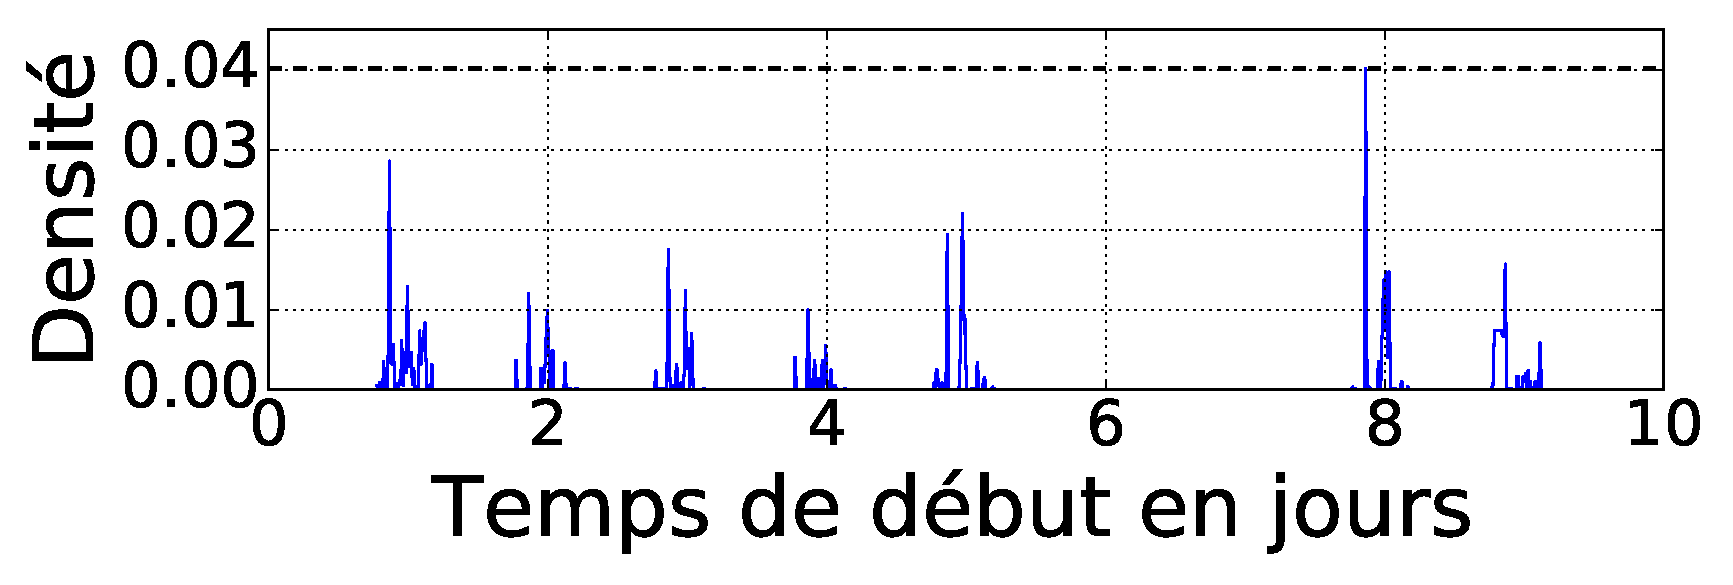
\includegraphics[width=\linewidth]{img/GroupeDense/GroupExample/SocioPattern/vairable_start9522.eps}
	\caption{}
	\label{fig:g9522_debut}
\end{subfigure}
\begin{subfigure}{0.45\linewidth}
	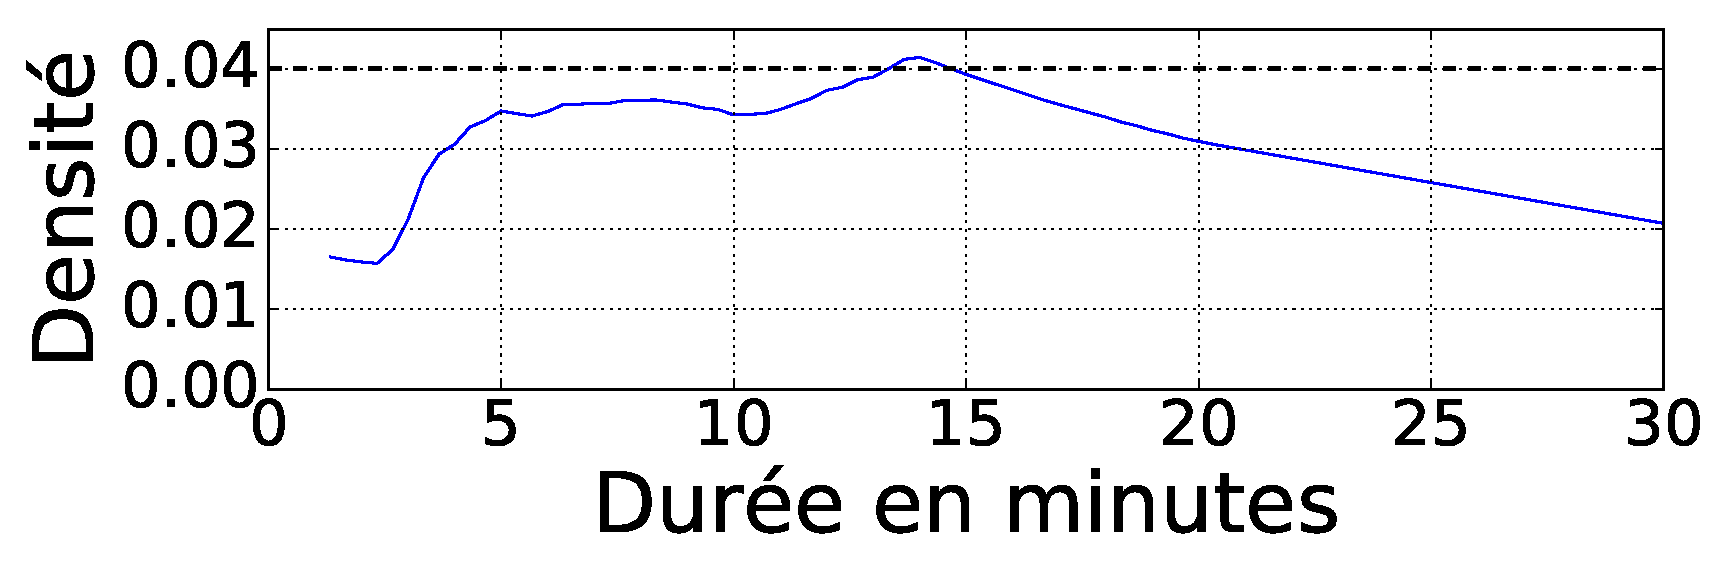
\includegraphics[width=\linewidth]{img/GroupeDense/GroupExample/SocioPattern/vairable_duration9522}
	\caption{}
	\label{fig:g9522_duree}
\end{subfigure}
\caption{
Densités du voisinage d'un groupe dans Socio Pattern.
En trait plein: la fonction $d(V(C_i),z,\bar{C_i})$ en (A) et la fonction  $d(V(C_i),\beta(C_i),y)$ en (B).
En pointillé, la densité du groupe est rappelée.
}
\label{fig:Sp_g9522_exemple}
\end{figure}

\subsubsection{Étude manuelle d'un groupe de Rollernet}
Dans les données Rollernet, nous connaissons le rôle des participants.
Certains des participants ne sont connus que comme membres d'une association de roller mais d'autres ont des rôles plus précis, \emph{e.g.} membre organisateur à l'arrière gauche du peloton.
Ce genre d'information aide lors de l'étude d'un groupe.
Le groupe que nous considérons contient $38$ liens, $9$ n\oe uds et dure pendant environ $5$ minutes.
Ce groupe de liens commence juste au début de la randonnée et $8$ des membres du groupe font partie des membres organisateurs à l'arrière de la randonnée.
Le dernier fait partie des membres organisateurs mais à l'avant.
Ce groupe pourrait indiquer une discussion rapide avant le début du tour.
Comme pour le groupe de Socio Pattern, nous analysons les scores obtenus par ce groupe.


\subsubsection*{Voisinage aux n\oe uds}
Pour ce voisinage, le groupe a un score de $0.99$ ce qui indique une fois de plus que cet ensemble de n\oe uds est important lorsque l'on considère le même intervalle de temps.
Il y a par ailleurs $477=9(62-9)$ sous-flots considérés pour ce candidat dans le voisinage aux n\oe uds.

\subsubsection*{Voisinage au temps de début}
Pour le voisinage au temps de début, le groupe a un score de $0.85$, voir la figure~\ref{fig:g7_debut}.
Comme le jeu de données Rollernet est plus court et plus dense que Socio Pattern, la densité est beaucoup plus stable en fonction du temps de début.
Cela se reflète d'ailleurs sur le score obtenu qui est plus faible.
Cependant comme le groupe de liens en question apparait 5 minutes après le début de la randonnée, il correspond tout de même à un maximum local de la densité.


\subsubsection*{Voisinage à la durée}
Pour le voisinage à la durée, le groupe a un score de $0.86$, voir la figure~\ref{fig:g7_duree}.
Encore une fois, le profil de la densité est plus lisse que dans le cas de Socio Pattern et une durée un peu plus courte donnerait lieu à une densité plus élevée. 
Enfin on remarque que, même si Rollernet est beaucoup plus dense que Socio Pattern, la densité décroît tout de même en fonction de la durée considérée.

\bigskip

Même si ces scores ne sont pas optimum et sont plus faibles que ceux obtenus dans l'exemple précédent, il faut les considérer dans le contexte du flot de liens de Rollernet.
Comme Rollernet est globalement plus dense, il est moins surprenant d'observer des sous-flots qui soient denses.
 

\begin{figure}
\centering
\begin{subfigure}{0.45\linewidth}
	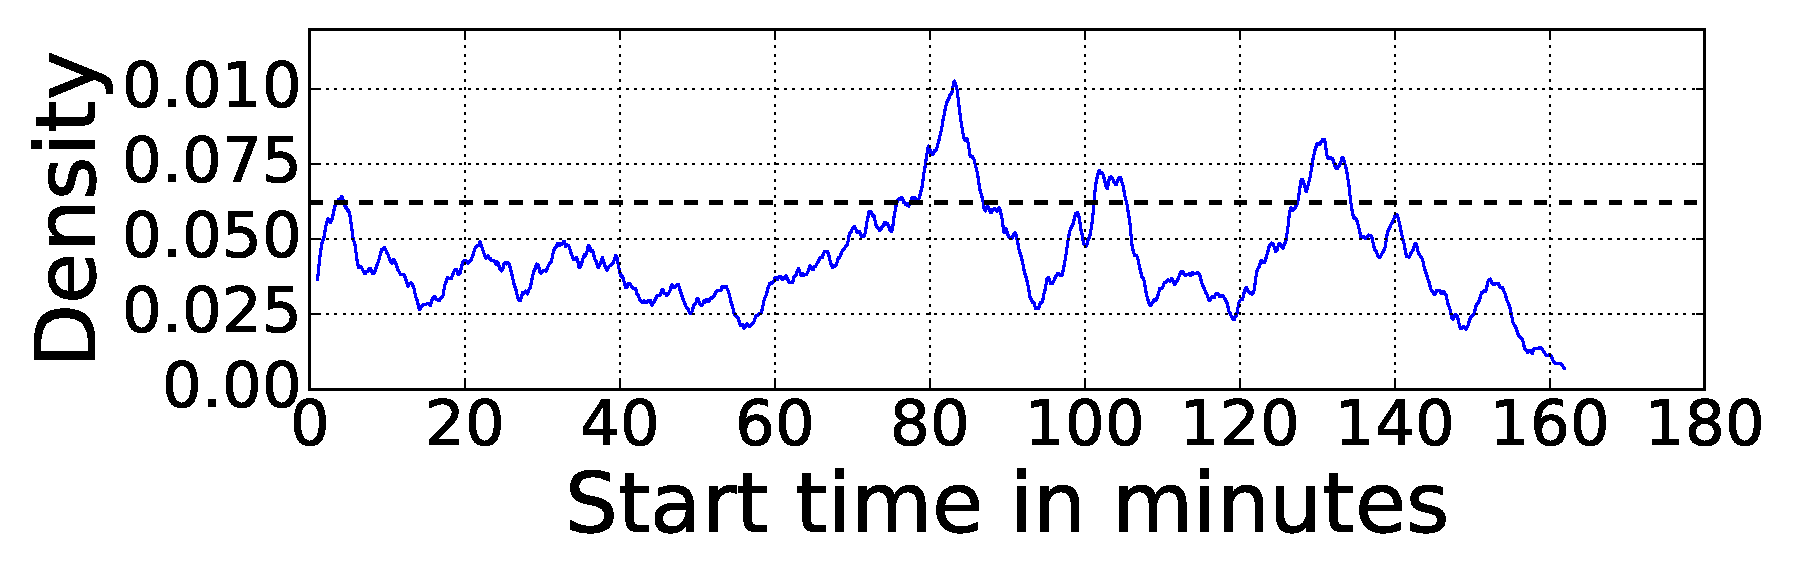
\includegraphics[width=\linewidth]{img/GroupeDense/GroupExample/Rollernet/vairable_start7}
	\caption{}
	\label{fig:g7_debut}
\end{subfigure}
\begin{subfigure}{0.45\linewidth}
	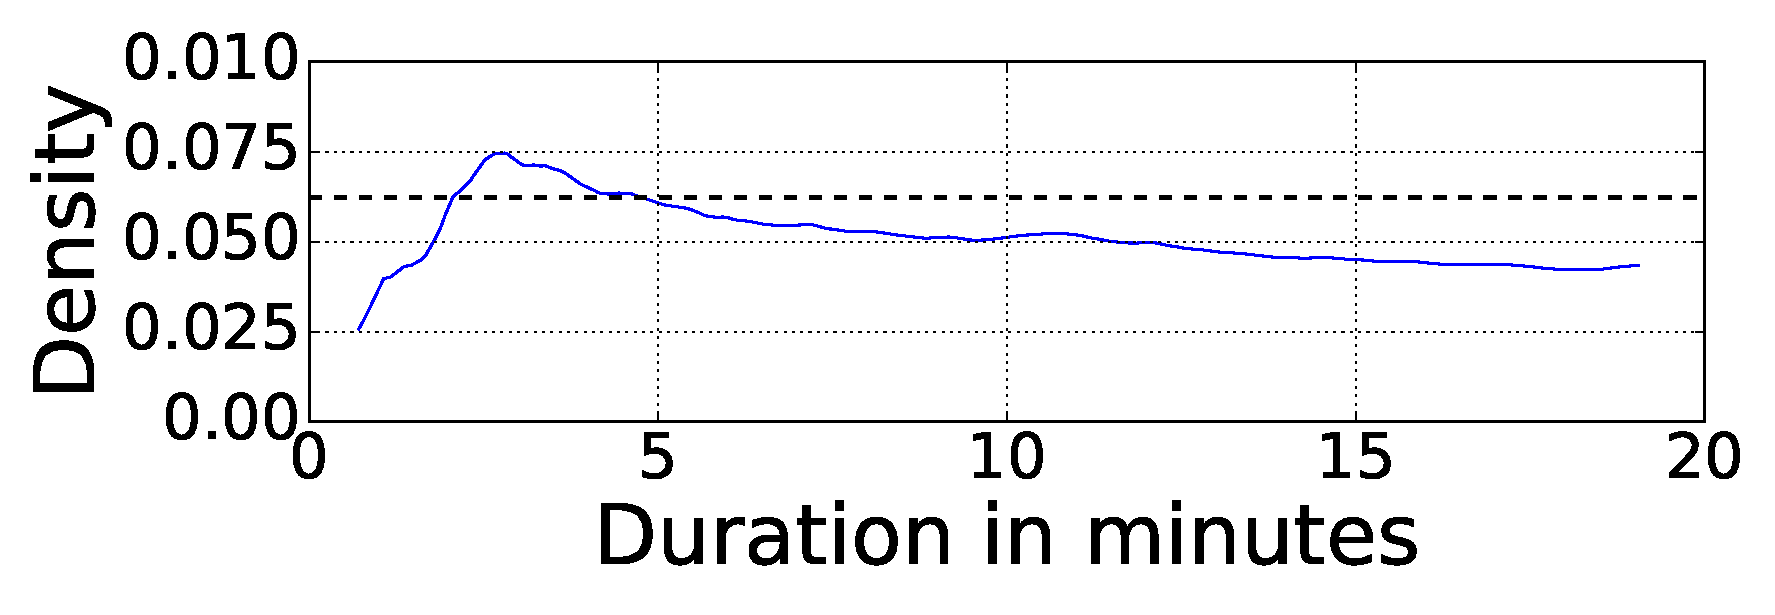
\includegraphics[width=\linewidth]{img/GroupeDense/GroupExample/Rollernet/vairable_duration7}
	\caption{}
	\label{fig:g7_duree}
\end{subfigure}
\caption{
Densités du voisinage d'un groupe dans Rollernet.
En trait plein: la fonction $d(V(C_i),z,\bar{C_i})$ en (A) et la fonction  $d(V(C_i),\beta(C_i),y)$ en (B).
En pointillé, la densité du groupe est rappelée.
}
\label{fig:Rollernet_exemple}
\end{figure}





\bigskip
Pour résumer, il y a $12\ 532$  groupes candidats initialement dans le cas de Socio Pattern.
Parmi eux, $155$ ont plus de $10$ liens et $136$ sont considérés comme pertinents.
La table~\ref{tab:res_exec} résume le nombre final de groupes pertinents capturés pour chaque jeu de données.


\begin{table}
\centering
\begin{tabular}{|c|c|c|}
\hline \rule[-1ex]{0pt}{3.5ex}
 & $N_c$ & temps d'exécution \\
\hline
Socio Pattern & 136 &  2 min \\
Rollernet& 37 &  4 min \\
Reality Mining & 394 & 1h \\
Babouin & 1023 & 52 min\\
\hline
\end{tabular}
\caption{$N_C$ nombre de groupes capturés et temps d'exécution pour chaque jeu de données}
\label{tab:res_exec}       % Give a unique label
\end{table}


Tous ces groupes ont des scores plus élevés que les seuils que nous avons fixés mais pour la plupart ils n'ont pas des scores parfaits.
Cela implique qu'il existe des sous-flots voisins ayant une densité plus importante.
C'est pourquoi nous avons également comparé la densité obtenue par le groupe à celle obtenue par le meilleur des sous-flots dans un voisinage donné.
Nous observons que dans $75\%$ des cas la densité des groupes est à moins de $20\%$ de l'optimal.
Cet écart est relativement stable selon les jeux de données et les voisinages.

Les groupes que nous considérons comme pertinents ont donc une densité proche de l'optimum quand bien même cet optimum n'est pas atteignable par un groupe de liens.
De plus, nous avons considéré les voisinages de manière séparée.
Or, il se peut par exemple que le sous-flot optimum dans le voisinage au temps de début ne soit pas l'optimum dans le voisinage à la durée.


\subsection{Caractéristiques des groupes pertinents}

Afin d'avoir une vision plus précise des groupes capturés comme pertinents, nous présentons les distributions cumulatives inverses du nombre de liens, de n\oe uds, de la durée et de la densité pour ces groupes dans la figure~\ref{fig:distri_group_SP_filter}.
Les distributions sont encore une fois hétérogènes sauf pour la densité.
Les distributions pour les autres jeux de données sont présentées en appendice pages \pageref{fig:distri_group_rollernet_filter} à \pageref{fig:distri_group_RM_filter} dans les figures~\ref{fig:distri_group_rollernet_filter},\ref{fig:distri_group_baboon_filter} et \ref{fig:distri_group_RM_filter}.
En plus de ces distributions, nous avons également étudié comment ces groupes de liens représentent le flot de liens et comment ils se répartissent dans le temps et la topologie du flot de liens.
Par exemple, les $136$ groupes pertinents du jeux de données Socio Pattern capturent $3\ 507$ liens, soit $17.7\%$ du flot de liens initial.
Les groupes pertinents sont donc bien une structure partielle du flot de liens.
Les valeurs de représentativité sont présentées dans la table~\ref{tab:res_representativite}.
On remarque notamment que même si peu de groupes sont capturés, ils représentent une plus grande proportion des liens du flots de liens pour les autres jeux de données.


\groupcharacFilter{Sociopattern}{Socio Pattern}{SP}{}
\begin{table}
\centering
\begin{tabular}{|c|c|c|c|c|}
\hline \rule[-1ex]{0pt}{3.5ex}
 & Socio Pattern & Rollernet  & Reality Mining & Babouin \\
\hline
Représentativité & $17.7\%$ & $95.4\%$ & $80.9\%$ & $39\%$ \\

\hline
\end{tabular}
\caption{Proportion de liens appartenant à un groupe pertinent (\emph{représentativité}) pour chaque jeu de données}
\label{tab:res_representativite}       % Give a unique label
\end{table}


\subsubsection{Caractéristiques topologiques}
Pour la répartition topologique des groupes, la distribution du nombre de groupes pertinents par n\oe ud est présentée dans la figure~\ref{fig:PropNode_SP} pour le jeu de données Socio Pattern.
Tous les n\oe uds appartiennent à au moins un groupe et quelques n\oe uds appartiennent même à plus de $20$ groupes.
Avec une moyenne de $7.4$ groupes par n\oe uds, les groupes pertinents forment donc une structure très recouvrante sur les n\oe uds.
Pour les autres jeux données voir les figures~\ref{fig:PropNode_rollernet},\ref{fig:PropNode_baboon} et \ref{fig:PropNode_RM}.
Nous observons également sur ces jeux de données un structure très chevauchante sur les n\oe uds, en particulier pour le jeu de donnée Babouin.
Cette différence est sûrement due au nombre relativement faible de n\oe uds comparé au nombre de liens: $28$ n\oe uds pour $95\ 616$ liens.

\bigskip

Il aurait peut-être été possible de détecter cette structure par une méthode capturant des communautés chevauchantes de n\oe uds dans un graphe.
Afin de tester cette hypothèse, nous créons un graphe agrégé pondéré tel que le poids d'un lien entre deux n\oe uds soit égal à la somme des durées des liens entre ces deux n\oe uds dans le flot de liens.
Ainsi, le poids des liens permet de garder une partie de l'information temporelle.
Pour la détection de communautés chevauchantes, nous avons utilisé l'algorithme bigclam proposé par Yang~\emph{et al.}~\cite{Yang2013}.
Nous l'avons décrit dans la section~\ref{subsec:cover}.
Cette méthode ne considère que des graphes non pondérés.
C'est pourquoi il est nécessaire de transformer le graphe pondéré en graphe non pondéré.
Comme aucune valeur singulière n'est apparue lors de l'étude de la distribution des poids des liens, nous avons avons créé plusieurs graphes non pondérés selon la règle suivante.
Un lien existe dans le graphe non pondéré si le poids associé au lien est supérieur ou égal à $\lambda\%$ des poids de tous les liens du graphe pondéré.
Ainsi en faisant varier $\lambda$, il est possible de prendre en compte dans une certaine mesure la pondération.
Une fois les graphes construits, nous appliquons l'algorithme \emph{bigclam} sur chaque graphe et obtenons des partitions chevauchantes de n\oe uds.

Nous utilisons l'indice de Jaccard afin de comparer les partitions chevauchantes obtenues par \emph{bigclam} et celle définie par les n\oe uds induits par les groupes pertinents.
L'indice de Jaccard, défini dans la section~\ref{sec:def_graphe}, nous permet de trouver, pour chaque groupe pertinent, le groupe trouvé par \emph{bigclam} qui est le plus proche.
La table~\ref{tab:Jaccard} liste les similarités médianes et maximales entre les groupes pertinents et ceux trouvés par \emph{bigclam} selon la valeur de $\lambda$ utilisée.
Lorsque l'on étudie cette table, on remarque que les groupes pertinents et les groupes trouvés par \emph{bigclam} sont différents car les indices de Jaccard médians sont très faibles.
Il y a toutefois quelques groupes pertinents qui sont retrouvés par \emph{bigclam} dans certains jeu de données.
Seulement, cela n'arrive que pour quelques valeurs de $\lambda$ et très peu de groupes.
C'est pourquoi notre méthode permet de mettre en valeur une structure des n\oe uds qui n'est pas retrouvée par une méthode classique sur le graphe agrégé.

\begin{table*}
\centering
\begin{tabular}{|c|c|c|c|c|c|c|}
\hline  \rule[-1ex]{0pt}{3.5ex}  & $\lambda= 0.05$ &$\lambda= 0.1$ & $\lambda=0.2$ & $\lambda=0.3$ & $\lambda=0.5$ & $\lambda=0.7$ \\ 
\hline Socio Pattern & 0.30 (0.55)  & 0.30 (0.55)  & 0.30 (0.55)  & 0.30 (0.55)  & 0.29 (0.54) & 0.33 (\textbf{0.85})  \\ 
\hline Rollernet & 0.40 (0.52) & 0.39 (0.64) & 0.41 (0.54) & 0.37 (0.54) & 0.31 (0.57)  &  0.26 (0.75) \\ 
\hline Reality Mining & 0.42 (0.76)  & 0.42 (0.77) & 0.36 (\textbf{0.88}) & 0.42 (\textbf{0.86}) & 0.38 (\textbf{0.87})  & 0.36 (\textbf{1}) \\ 
\hline Baboons & 0.33 (\textbf{0.95}) & 0.38 (\textbf{1}) & 0.40 (\textbf{0.84}) & 0.46 (\textbf{0.94}) & 0.46 (\textbf{0.93}) & 0.44 (\textbf{0.85}) \\ 
\hline 
\end{tabular} 
\caption{Indice de Jaccard médian (et maximum) entre les groupes pertinents et les groupes trouvés par \emph{bigclam} dans le graphe agrégé où les liens ayant un poids inférieur à $\lambda\%$ des liens ont été retirés.
Les indices de Jaccard supérieurs à $0.8$ sont en gras.}
\label{tab:Jaccard}  
\end{table*}

\subsubsection{Caractéristiques temporelles}
Pour l'aspect temporel, nous avons également étudié le chevauchement temporel entre les groupes pertinents.
Pour ce faire, nous regardons la proportions du temps durant laquelle il n'existe aucun groupe présent.
Pour tous les jeux de données excepté Rollernet, entre $82\%$ et $95\%$ du temps il n'y a aucun groupe présent.
Cette proportion élevée s'explique par la nature des jeux de données qui couvrent de longue périodes, ce qui inclut des nuits où aucun lien n'apparaît.
Pour le jeu de donnée Rollernet, cette proportion de temps sans groupe pertinent n'est que de $15\%$.

De manière plus importante, il existe également des instants où plusieurs groupes pertinents sont présents.
Dans le jeu de données Socio Pattern, c'est notamment le cas lors des pauses ou des repas le midi.
Durant ces instants, il peut y avoir jusqu'à quatre groupes présents en même temps.
Ces instants importants sont visibles via notre méthode mais ils sont bien évidemment facilement identifiables par d'autres méthodes plus simples telles que le degré temporel.

De manière globale, la structure temporelle des groupes pertinents est très différente de la structure topologique car une part importante du temps n'est impactée par aucun groupe pertinent.
Il est toutefois intéressant de noter que les deux structures sont chevauchantes. 



\section{Conclusion et perspectives}
\subsection{Conclusion}

Dans ce chapitre, nous nous sommes intéressés à la détection de groupes de liens pertinents dans un flot de liens.
\`A l'inverse des méthodes existantes, nous considérons pleinement l'information temporelle et nous n'utilisons aucune agrégation pour évaluer nos résultats.
Cette différence a été permise par l'utilisation du formalisme de flot et de ses métriques mélangeant vraiment structure et temps.
De plus, notre méthode ne capture pas des ensembles de n\oe uds et des intervalles de temps mais des ensembles de liens.

Pour capturer des groupes de liens, nous avons proposé une transformation du flot de liens en un graphe statique non pondéré tel que les liens sont transformés en n\oe uds dans le graphe.
Deux n\oe uds dans le graphe sont reliés si les liens correspondants dans le flot ont au moins un n\oe ud et un instant de temps en commun.
C'est pourquoi, rechercher une communauté dans le graphe statique permet de trouver des groupes liens connectés temporellement et structurellement.
Nous utilisons l'algorithme de Louvain qui permet de capturer des partitions de n\oe uds dans un graphe.
Nous obtenons ainsi un ensemble de groupes de liens potentiellement pertinents.

Afin de trouver les groupes pertinents parmi l'ensemble des groupes de la partition trouvée par Louvain, nous avons proposé un critère évaluant la pertinence du sous-flot défini par les liens du groupe.
Un sous-flot est jugé pertinent en fonction de scores comparant la densité du sous-flot et la densité des sous-flots proches temporellement et topologiquement.
Un sous-flot peut être caractérisé par les n\oe uds participants à ce sous-flot, l'instant d'apparition du premier lien du sous-flot et la durée du sous-flot.
Il est donc naturel de considérer trois voisinages.
Chaque voisinage est alors composé de sous-flots différant du sous-flot initial sur un seul aspect: l'ensemble de n\oe uds, le temps début ou la durée.
Le score d'un groupe de liens dans un voisinage est ainsi défini par la proportion de sous-flots étant moins denses que lui.
Finalement, le groupe de liens est jugé pertinent si ces scores sont plus élevés que des seuils qui sont fixés \emph{a posteriori}.
Ainsi, modifier ces seuils ne modifient pas les groupes candidats mais uniquement les groupes qui sont jugés pertinents.


Nous avons appliqué notre méthode sur quatre jeux de données réels représentant des interactions entre individus.
Deux d'entre eux sont des interactions entre étudiants.
Un est un réseau de participant à une randonnée roller à Paris et le dernier est un réseau de babouins.
Ils proviennent ainsi de contextes radicalement différents.
Cela se traduit notamment sur la densité  globale des flots de liens.
Pour tous ces jeux de données, nous avons réussi à capturer des groupes ayant des scores très élevés.

La validation de ces résultats est délicate car il n'existe pas de vérité de terrain sur ces données et il n'existe aucun algorithme similaire.
Cependant il existe des méta-données pour deux des jeux de données.
De cette manière, nous avons pu analyser manuellement quelques groupes considérés comme pertinents par notre méthode.
Nous avons observé que les groupes étudiés correspondaient à des événements existants dans ces jeux de données comme le regroupement d'étudiants avant le premier cours de la semaine.
Nous avons également étudié comment l'ensemble des groupes pertinents se répartissent dans le temps et la topologie du réseau.
Nous avons observé qu'ils sont très chevauchants sur les n\oe uds et sur le temps mais qu'ils ne concernent cependant qu'une fraction du temps total.


Afin de tester la nouveauté de la structure que nous capturons, nous avons appliqué un algorithme de détection de communautés chevauchantes, \emph{bigclam}, sur le graphe agrégé.
Il apparait que parmi l'ensemble des groupes pertinents seulement quelques un sont retrouvés par \emph{bigclam}.
Ce résultat illustre l'importance de prendre en compte le temps lors de l'étude d'un réseau.


\subsection{Perspectives}

Notre méthode repose sur la projection du flot de liens en un graphe statique, d'une méthode de détection de communauté, une taille de groupe minimum et des seuils qui sont fixé \emph{a posteriori}.
Les axes de recherche associés à ces travaux sont principalement de deux types: l'amélioration de la détection des groupes pertinents et l'amélioration de la validation des groupes détectés.

\subsubsection{Amélioration de la détection des groupes pertinents}
Notre méthode n'est pas encore automatique car il est nécessaire de fixer les seuils des scores et la taille minimum d'un groupe.
La taille minimum ne semble pas être très délicate à choisir.
Il serait intéressant de voir si notre méthode est capable de filtrer automatiquement les petits groupes.
Nous n'avons cependant pas encore poursuivi cet axe de recherche car la prise en compte des petits groupes impacterait fortement la distribution des scores et donc le choix des seuils.
De plus, les seuils nécessitent déjà une connaissances des données.

C'est pourquoi, il serait intéressant de pouvoir automatiser le choix de seuil.
Lors de l'application de notre méthode, nous avons à chaque fois observé une forte décroissance dans la distribution des scores.
Une méthode prometteuse serait donc de se baser sur la détection de point d'inflexion pour déterminer les seuils.
Il est par exemple possible de détecter les moments où la dérivée seconde est nulle.
Cependant, le comportement que nous avons observé n'est pas forcément universel et il faudrait donc étudier des flots de liens provenant de différents contextes avant de généraliser cette approche.


Il serait également intéressant de remettre en question la méthode de détection utilisée.
Nous utilisons l'algorithme de Louvain sur la projection du flot de liens en un graphe statique.
D'une part, il est possible d'utiliser d'autres algorithmes de détection de communautés en tant que partition de n\oe uds tels que ceux listés dans la sous-section~\ref{subsec:Part_noeuds}.
Mais il est également possible de considérer les couvertures comme une liste de candidats potentiels.
Il serait par exemple possible d'appliquer \emph{bigclam} sur la projection.
D'autre part, il est également nécessaire de réfléchir à l'impact sur les groupes candidats de l'utilisation de la projection du flot en un graphe car il est possible qu'un groupe pertinent ne soit pas détectable dans la projection.
En effet, un lien dans la projection nécessite notamment un chevauchement temporel des liens dans le flot de liens.
Si deux liens sont séparés par un intervalle de temps, alors ils ne seront pas reliés dans la projection peu importe la durée de l'intervalle les séparant.
Il serait donc intéressant de détecter directement les groupes pertinents.

Il n'est pas possible, à partir de la projection, de calculer la densité et les voisinages d'un groupe de lien.
Il est donc nécessaire de manipuler directement un flot de liens pour espérer trouver les groupes pertinents.
Comme l'évaluation d'un groupe de liens est locale, une approche locale intégrant au fur et à mesure des liens dans un groupe candidat est envisageable.
Le but est alors d'améliorer un groupe jusqu'à obtenir un équilibre de Nash, c'est à dire qu'il ne soit pas possible d'améliorer un score sans dégrader les deux autres.
Même si cette approche ne permet pas la détection directe de groupes pertinent, il serait intéressant d'améliorer localement les groupes candidats proposés par l'algorithme de Louvain.


\subsubsection{Amélioration de la validation des résultats}

Nous avons comparé nos résultats uniquement à une méthode statique car les méthodes de l'état de l'art sur les réseaux dynamiques manipulent principalement des séries de graphes .
Or, le changement de formalisme impacte fortement l'objet d'étude.
Dans une série de graphes, il y a une agrégation temporelle.
L'identité d'un lien est donc perdue lors de l'agrégation et il est ainsi délicat de comparer des groupes de liens dans un flot de liens et des groupes de n\oe uds dans une série de graphes.
Pour pouvoir appliquer les méthodes de série de graphes, il est donc d'abord nécessaire de construire une ou plusieurs transformations du flot de lien en série de graphes.
\`A partir de cette série de graphes, il est alors possible d'appliquer les méthodes existantes pour trouver des communautés dans chaque graphe.
Il serait alors intéressant de calculer les scores obtenus par les sous-flots induit par les n\oe uds d'une communauté sur l'intervalle de temps où la communauté à été détectée dans la série de graphes.


Cette approche permettrait de comparer plus en profondeur les résultats mais pas de les valider.
Comme il n'existe pas de données avec une vérité de terrain, une approche prometteuse serait de créer des modèles génératifs de flots de liens permettant de définir des contraintes sur la densité.
Ainsi, il serait alors possible de tester de manière quantitative notre méthode.
Cela permettrait de plus d'ouvrir la voie pour des méthodes de détection de communautés de liens dans les flots de liens.
Nous abordons le problème de la détection de communautés de liens dans les graphes dans le chapitre suivant et nous esquissons des pistes de générations de flots de liens avec une structure dans le chapitre~\ref{versQualite}.

\chapter{\emph{Expected Nodes}: communautés de liens dans les graphes statiques}
\minitoc

\label{chap:Expected_Node}
Nous avons vu précédemment une méthode de détection de partitions partielles de liens dans les flots de liens.
Avant de considérer les partitions complètes de liens dans les flots de liens, il est important de comprendre les méthodes existantes dans le cas statique.
Les structures communautaires dans les graphes ont été beaucoup étudiées lorsqu'elles concernent les n\oe{}uds, voir le chapitre~\ref{chap:etat_art}.
Dans une moindre mesure, elles ont également été étudiées lorsqu'elles concernent les liens.
Par exemple dans un réseau social, chaque personne a plusieurs centres d'intérêt: famille, sport, politique...
Lorsque deux personnes interagissent, la communication a lieu dans un contexte bien particulier.
Bien que les personnes aient plusieurs centres d'intérêts, la raison de leur communication est souvent unique.
Il semble donc qu'une information importante soit intrinsèquement liée au lien.
Via la recherche de partitions de liens d'un graphe, c'est cette information que nous cherchons à capturer.

\begin{figure}
\centering
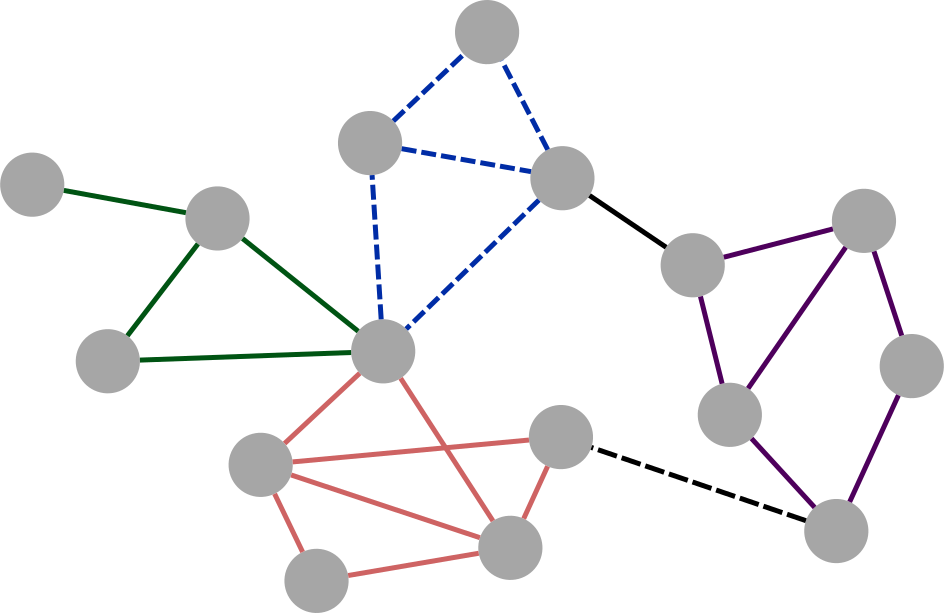
\includegraphics[width=0.5\linewidth]{img/ExpectedNodes/Link_Partition}
\caption{Exemple de réseau de personnes avec une structure communautaire sur les liens qui est représentée par la couleur et le style de chaque lien.}
\label{fig:linkpartition_exemple_expected}
\end{figure}
Afin d'illustrer ce que capture une partition, prenons l'exemple d'un réseau de personnes fictif où le contexte de l'interaction est connu.
Certaines personnes communiquent ensemble car elles sont de la même \textbf{\textcolor{bleu_random}{famille}}, pratiquent le même \textbf{\textcolor{rose_cochon}{sport}}, jouent au \textbf{\textcolor{vert_fonce}{go}} ensemble ou bien encore car elles \textbf{\textcolor{violet_cool}{travaillent}} ensemble.
Nous illustrons cet exemple dans la figure~\ref{fig:linkpartition_exemple_expected} où les interactions sont colorées en fonction de leur contexte.
Il est intéressant de noter que les interactions d'un même type se regroupent ensemble.
Un n\oe{}ud peut avoir des interactions de plusieurs types; c'est le cas du n\oe{}ud central qui a des interactions de type \textbf{\textcolor{bleu_random}{famille}}, \textbf{\textcolor{rose_cochon}{sport}} et \textbf{\textcolor{vert_fonce}{go}}.
De même, certaines interactions font le lien entre différent groupes.
C'est le cas du lien pointillé \textbf{noir} qui relie le \textbf{\textcolor{rose_cochon}{sport}} et le \textbf{\textcolor{violet_cool}{travail}} ce qui pourrait se traduire par le financement de l'équipe par l'entreprise.
Ainsi, les partitions de liens peuvent capturer des situations assez variées.

Il est également possible de manipuler des partitions chevauchantes ou couvertures.
Dans ce cas, chaque n\oe{}ud peut appartenir à plusieurs communautés.
Face à ce problème de nombreux algorithmes ont été proposés pour la détection et l'évaluation de couvertures de n\oe{}uds, voir la section~\ref{subsec:cover}.
Les couvertures sont une généralisation des partitions et aucune méthode ne fait encore consensus pour les évaluer car leur structure est complexe.
Les partitions de liens, quant à elles, restent des objets plus simples à manipuler.
De plus, elles permettent de mettre en avant une autre structure ayant également du sens.



Il apparaît donc que les partitions de liens sont des objets à part entière.
Pour les étudier, il est nécessaire d'adapter les outils d'analyse pour évaluer directement les partitions de liens.
Nous développons ici une approche similaire à ce qui est fait pour les partitions de n\oe{}uds et la modularité~\cite{Newman2004}.
Le but est de créer une fonction de qualité permettant d'évaluer une partition de liens d'un graphe.

Dans la suite, nous utiliserons les notations suivantes.
Soit $G=(V,E)$ un graphe non-orienté avec $V$ l'ensemble des n\oe{}uds de taille $n$ et $E \subseteq V \times V$ l'ensemble des liens de taille $m$. 
Le degré d'un sommet $u$ de $G$ est noté $d_G(u)$.
Une partition des liens en $k$ groupes est notée $\mathcal{L}=(L_1,L_2,\ldots,L_k)$ avec $L_i \subseteq E \ \forall i$, $L_i\cap L_j=\emptyset \ \forall i\neq j$ et $\bigcup_i L_i=E$.
Pour un groupe de liens $L \in \mathcal{L}$, on pose $V_{in}=\{u \in V, \exists (u,v) \in L\}$ l'ensemble des n\oe{}uds internes au groupe $L$, $V_{out}=\{u \in V\setminus V_{in}, (u,v) \in E \wedge v \in V_{in} \}$ représente les n\oe{}uds adjacents au groupe $L$ et enfin $L_{out}=\{(u,v) \in E \setminus L, u \in V_{in} \vee v \in V_{in} \}$ l'ensemble des liens adjacents au groupe $L$ (voir la figure~\ref{fig:example_def_expected}).

\section{Travaux existants}
\label{sec:expected_travaux}
\begin{figure}
\centering
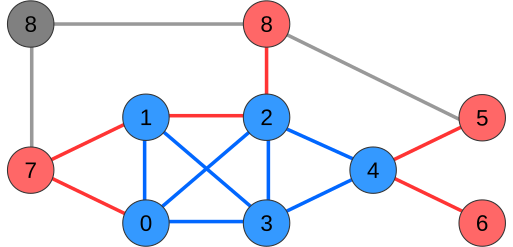
\includegraphics[width=0.4\linewidth]{img/ExpectedNodes/exemple2}
\caption{Exemple d'un groupe de liens $L$ (en \textcolor{semilightblue}{\textbf{bleu}}). Les liens \textcolor{pinkyred}{\textbf{rouges}} sont les liens adjacents $L_{out}$.
Les n\oe{}uds internes $V_{in}$ sont en \textcolor{semilightblue}{\textbf{bleu}} et les n\oe{}uds adjacents $V_{out}$ en \textcolor{pinkyred}{\textbf{rouge}}.}
\label{fig:example_def_expected}
\end{figure}

Une approche naïve serait de transformer le graphe initial en un \emph{line-graph}.
Un \emph{line-graph} est un graphe où chaque lien du graphe initial est transformé en un n\oe{}ud dans le \emph{line-graph}.
Deux n\oe{}uds du \emph{line-graph} sont reliés si les liens correspondants ont au moins un n\oe{}ud en commun, voir la figure~\ref{fig:ex_construction_lineG}.
Comme un \emph{line-graph} est un graphe classique, on peut y appliquer toutes les méthodes déjà existantes, \emph{e.g.} les algorithmes de détection de communautés.
Ainsi, une partition des n\oe{}uds du \emph{line-graph} représente une partition des liens du graphe initial.
Sur l'exemple de la figure~\ref{fig:ex_construction_lineG}, les liens $(1,4)$, $(1,3)$ et $(4, 3)$ du graphe forment un triangle dans le \emph{line-graph} et pourraient être capturés comme étant une communauté.
Ces liens dans le graphe initial forment également un triangle et peuvent être considérés comme une communauté valide.
\begin{figure}
\centering
	\begin{subfigure}{0.25\textwidth}
		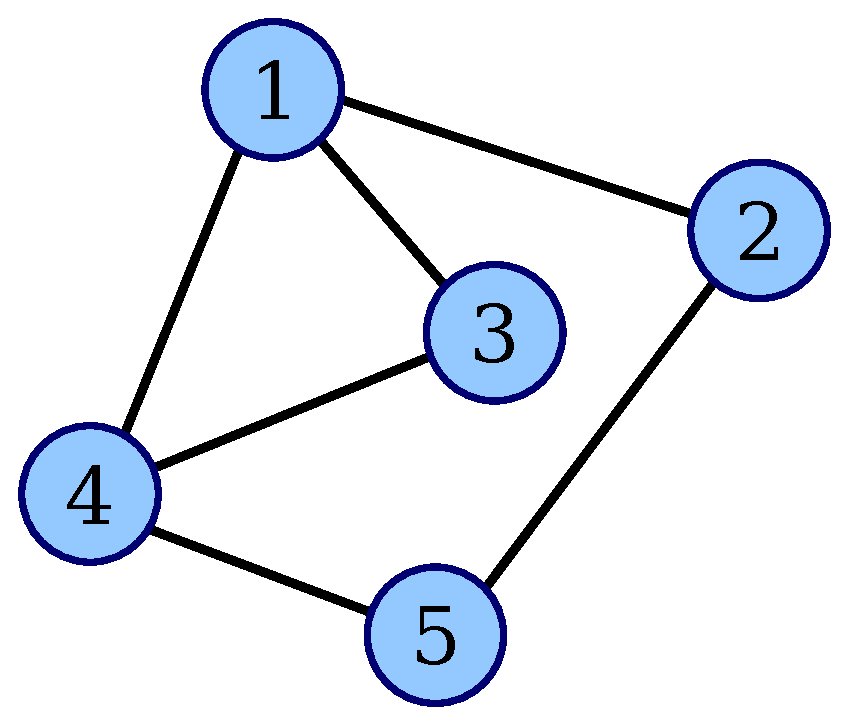
\includegraphics[height=3cm]{img/ExpectedNodes/Line_graph_construction_1.eps}
		\caption{Graphe initial}
	\end{subfigure}\hspace*{0.5cm}
	\begin{subfigure}{0.25\textwidth}
		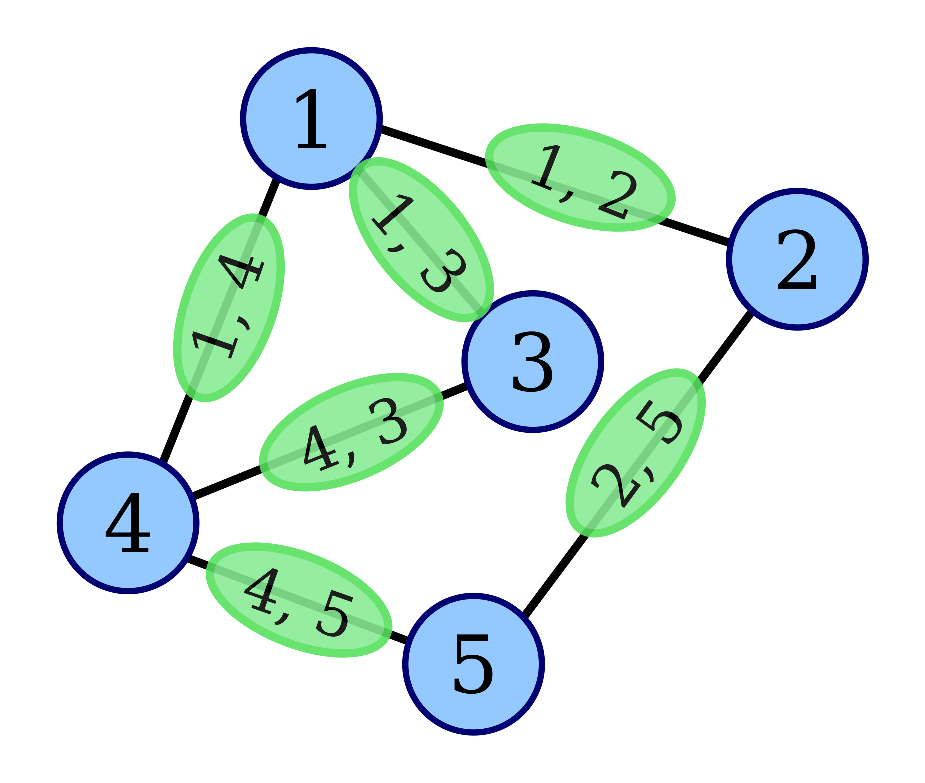
\includegraphics[height=3cm]{img/ExpectedNodes/Line_graph_construction_2.eps}
		\caption{Définition des n\oe{}uds du \emph{line-graph}}
	\end{subfigure}\hspace*{0.5cm}
	\begin{subfigure}{0.25\textwidth}
		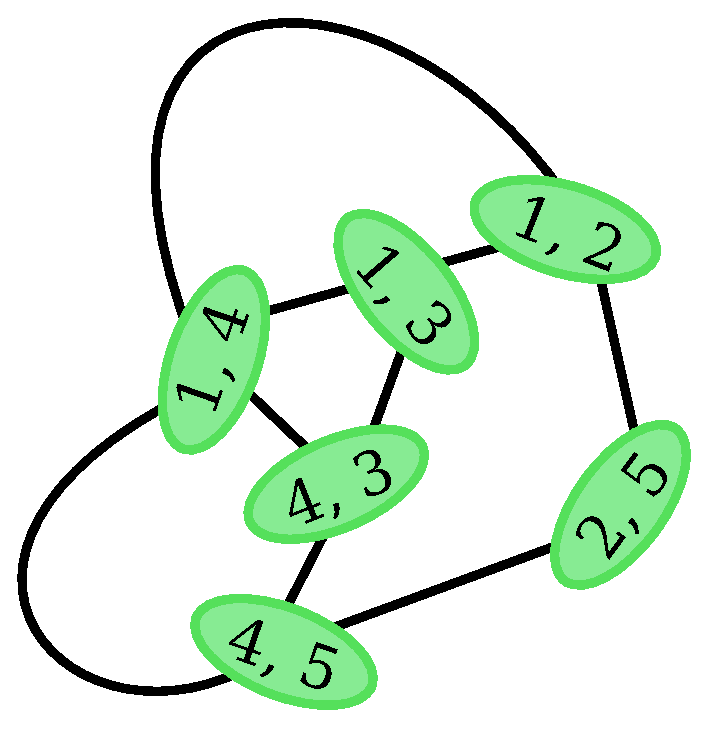
\includegraphics[height=3cm]{img/ExpectedNodes/Line_graph_construction_3.eps}
		\caption{Définition des liens du \emph{line-graph}}
	\end{subfigure}	
	\caption{Exemple de construction du \emph{line-graph}\,\protect\footnotemark.}
	\label{fig:ex_construction_lineG}
\end{figure}
\footnotetext{Image provenant de \url{https://en.wikipedia.org/wiki/Line_graph}.}

Cependant pour que ce type de méthode fonctionne, il est nécessaire que le \emph{line-graph} résultant puisse être analysé comme un graphe.
En particulier, il est nécessaire que la notion de communauté dans le \emph{line-graph} ait un sens dans le graphe initial.
Or, un \emph{line-graph} a une structure très différente du graphe initial.


Prenons pour l'exemple, la clique qui est la meilleure communauté possible et l'étoile qui est une des pires communautés possibles.
Le but est d'observer comment ces structures sont transformées dans le \emph{line-graph}.
Ces situations sont représentées dans la figure~\ref{fig:fail_construction_lineG}.
L'étoile dans la figure~\ref{fig:ex_lineG_etoile} est transformée en une clique de 4 n\oe{}uds.
Une des pires structures communautaires d'un graphe est transformée dans le \emph{line-graph} en la meilleure structure communautaire.
En effet, chaque n\oe{}ud de degré $k$ du graphe initial donne lieu à une clique de taille $k$ dans le \emph{line-graph}.
Les cliques du \emph{line-graph} ne sont donc pas forcément des communautés dans le graphe.
Dans le cas de la clique de taille $4$ dans la figure~\ref{fig:ex_lineG_clique}, on remarque que le \emph{line-graph} est composé de $6$ n\oe{}uds et de uniquement $12$ liens.
Plus généralement une clique de taille $n$ dans le graphe initial donne lieu dans le \emph{line-graph} à $\dfrac{n(n-1)}{2}$ n\oe{}uds et $(n-1)n$ liens.
Ainsi, plus la clique est grande dans le graphe, moins la structure résultante dans le \emph{line-graph} est dense.
Les cliques du graphe sont donc moins denses que ses étoiles, lorsqu'on les observe dans le \emph{line-graph}.

Il n'est donc pas trivial d'utiliser le \emph{line-graph} pour trouver des communautés de liens.
Il est nécessaire d'adapter les outils à ce type de graphe.
\begin{figure}
\centering

	\begin{subfigure}{0.4\textwidth}
		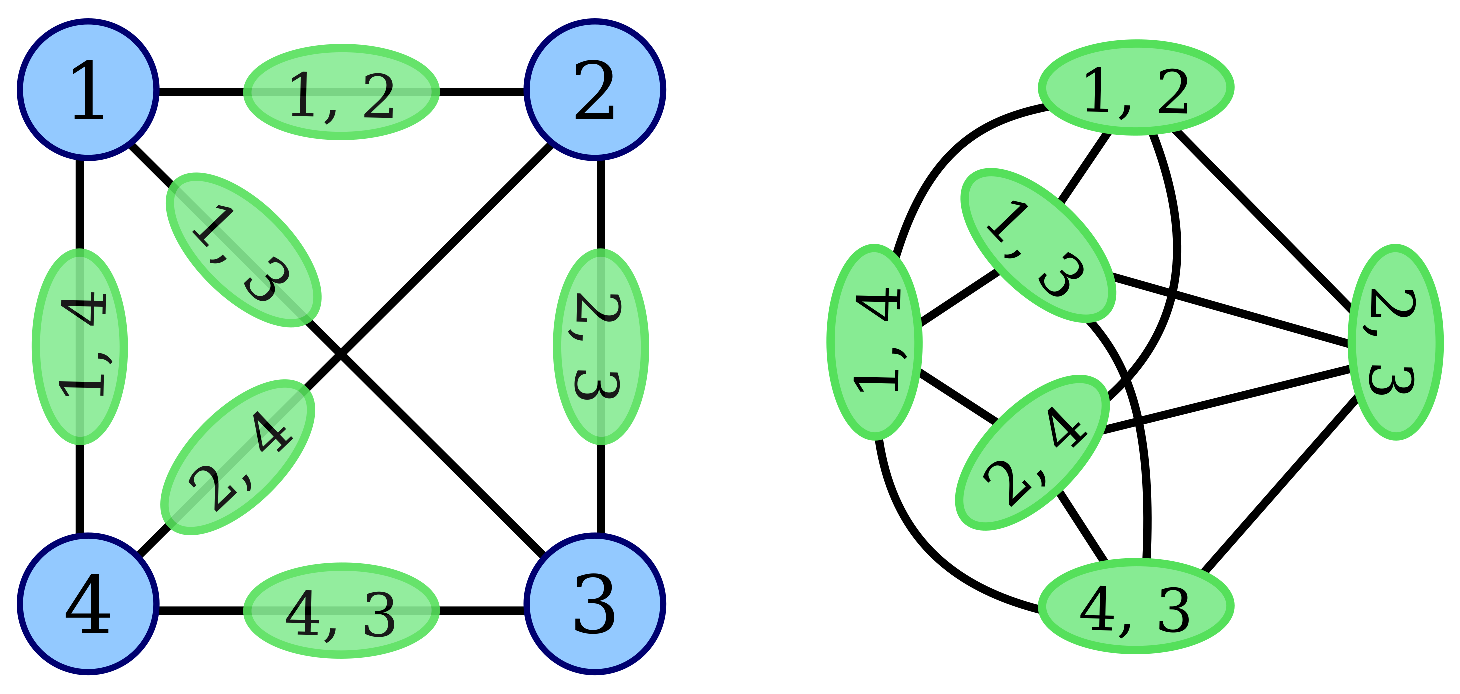
\includegraphics[height=3cm]{img/ExpectedNodes/Example/transfo_clique}
		\caption{}
		\label{fig:ex_lineG_clique}	
	\end{subfigure}\hspace*{0.1\textwidth}
	\begin{subfigure}{0.4\textwidth}
		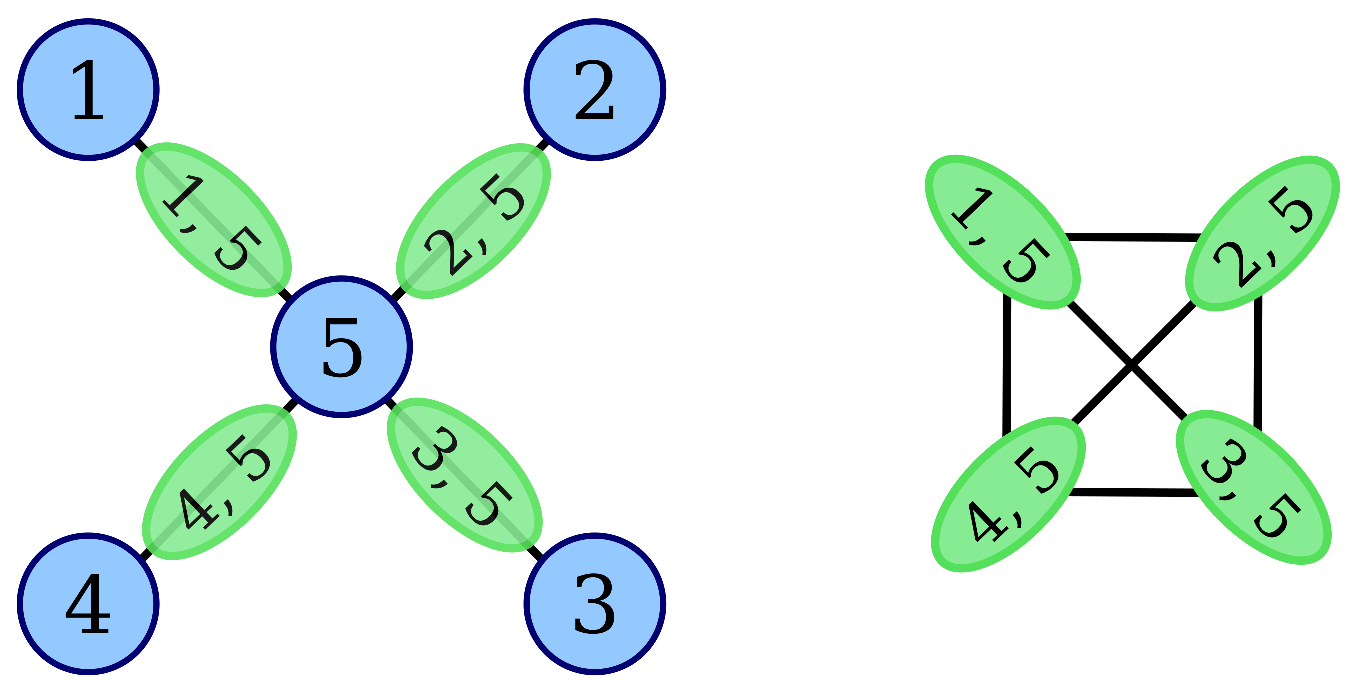
\includegraphics[height=3cm]{img/ExpectedNodes/Example/transfo_etoile}
		\caption{}
		\label{fig:ex_lineG_etoile}	
	\end{subfigure}
	

	\caption{Exemple de construction du \emph{line-graph} d'une clique en (A) et d'une étoile en (B).}
	\label{fig:fail_construction_lineG}
\end{figure}




Il existe d'autres méthodes que le \emph{line-graph} pour la détection et l'évaluation de partitions de liens.

Les algorithmes de propagation de labels ont été étendus pour capturer des partitions de liens~\cite{Yu2013}
Cependant, ils ne permettent pas d'évaluer la qualité de la partition obtenue.

Il y a les méthodes évaluant une partition de liens via la transformation de la partition en une couverture de n\oe{}uds~\cite{Huang2013,Lim2014,Wu2010a}.
Une transformation classiquement utilisée est qu'un n\oe{}ud dans la couverture prend comme communautés l'ensemble des communautés de ses liens, voir la figure~\ref{fig:Partition_Couverture}.
Il serait alors tentant de considérer que les partitions de liens et les couvertures de n\oe{}uds sont équivalentes.
Ainsi pour évaluer une partition de liens, il suffirait de transformer la partition en couverture.
Or, ce changement n'est pas anodin.
D'une part, les couvertures de n\oe{}uds permettent de modéliser beaucoup plus de situations car il n'y a aucune contrainte sur les couvertures.
D'autre part, transformer une partition de liens en couverture de n\oe{}uds impose des contraintes sur la couverture résultante.

\begin{figure}
\centering
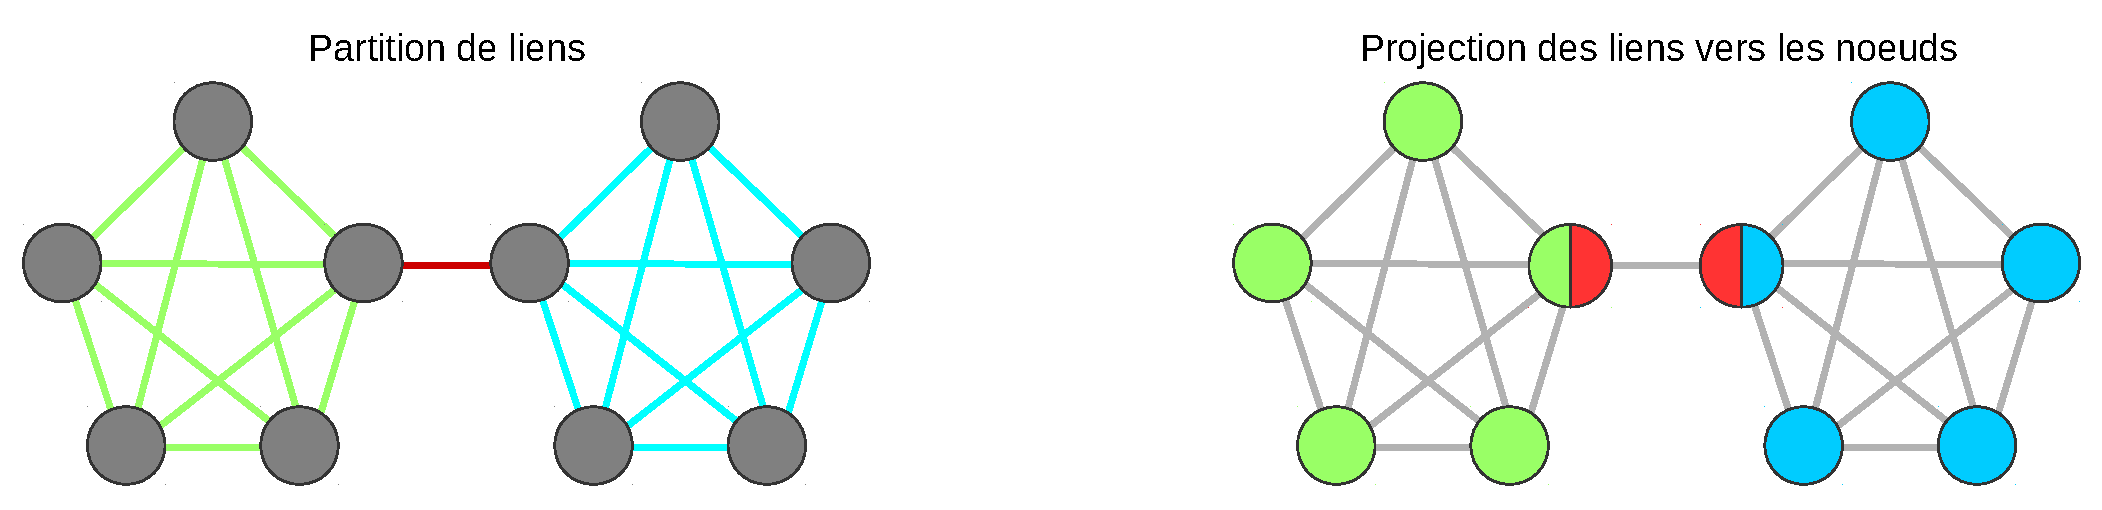
\includegraphics[width=0.9\linewidth]{img/ExpectedNodes/Partition_Couverture}
\caption{Transformation d'une partition de liens à gauche en couverture de n\oe{}uds à droite. La couleur représente un groupe.}
\label{fig:Partition_Couverture}
\end{figure}


Par exemple dans l'exemple de la figure~\ref{fig:Partition_Couverture}, il n'est pas évident que la communauté \textcolor{briquered}{\textbf{rouge}} constituée des deux n\oe{}uds centraux soit une communauté légitime.
Selon le contexte, elle peut être considérée comme un artefact de la transformation.
La transformation d'une partition n'est donc pas un acte neutre.
Cet aspect a d'ailleurs été mis en avant par Esquivel et Rosvall~\cite{Esquivel2011}.
Face à ce problème, nos travaux ainsi que quelques méthodes existantes proposent des méthodes évaluant directement les partitions de liens.

Ahn \emph{et al.}~\cite{Ahn2010a} sont parmi les premiers à avoir proposé une méthode détectant les communautés de liens.
Leur méthode \emph{link clustering} est une méthode hiérarchique d'agglomération.
Elle construit un dendrogramme en agglomérant de manière itérative les groupes de liens en fonction de leur similarité, calculée par l'indice de Jaccard.
Afin de décider de la coupe du dendrogramme et de la partition résultante, la fonction \emph{Partition Density} est utilisée.
Pour une partition de liens donnée $\mathcal{L}$, la \emph{Partition Density} est définie de la manière suivante:
\begin{equation}
D(\mathcal{L}) = \dfrac{\sum_{L \in \mathcal{L}}|L|D(L)}{m},\ avec \quad  D(L) = \dfrac{|L|- min_D(|V_{in}|) }{max_D(|V_{in}|) - min_D(|V_{in}|)},
\end{equation}

où $min_D(N) = N - 1$ est le nombre minimum de liens nécessaire pour relier $N$ n\oe{}uds et $max_D(N) = \dfrac{N(N - 1)}{2}$ est le nombre maximum de liens qui puissent exister entre $N$ n\oe{}uds.
Malgré son nom la \emph{Partition Density} n'est pas une densité mais le nombre de liens du groupe normalisé par le nombre de liens minimum et maximum possible pour un groupe de $|V_{in}|$ n\oe{}uds.
Après simplification, on obtient la formule suivante:

\begin{equation}
 D(L) = 2 \dfrac{|L| - (|V_{in}|-1) }{(|V_{in}|-1) (|V_{in}|-2)}.
\end{equation}

Par convention, un groupe constitué d'un unique lien, et qui n'a donc que deux n\oe{}uds internes, a une qualité nulle.

D'autres chercheurs~\cite{Li2013,Shi2013} ont par la suite utilisé la \emph{Partition Density} comme fonction à optimiser dans des algorithmes génétiques.
Leurs solutions semblent pour l'instant difficilement utilisables car leurs algorithmes reposent sur de nombreux critères et sont limités à de petits graphes.

Par ailleurs, la \emph{Partition Density} ne peut pas être directement appliquée aux graphes pondérés.
Une première proposition de Kim et Kim~\cite{Kim2014a} a été faite dans ce sens.




Evans et Lambiotte~\cite{Evans2009} proposent trois fonctions de qualité pour évaluer les partitions de liens.
Leurs fonctions de qualité sont basées sur trois marches aléatoires qui se déroulent sur les liens du graphe.
L'approche est similaire à la modularité car la modularité peut également être définie à l'aide d'une marche aléatoire sur les n\oe{}uds du graphe~\cite{Delvenne2010}.
Leurs trois fonctions de qualité peuvent être calculées et optimisées sur le graphe mais les auteurs ont montré que l'on pouvait, de manière complètement équivalente, utiliser la modularité sur des \emph{line-graph} pondérés ($LG_1$, $LG_2$, $LG_3$).
Ainsi, il suffit de construire le \emph{line-graph} approprié puis d'utiliser un algorithme existant d'optimisation de la modularité tel que l'algorithme de \emph{Louvain}~\cite{Blondel2008a}.


Pour construire les \emph{line-graphs} $LG_1$, $LG_2$ et $LG_3$, nous définissons $B\in \mathcal{M}_{n,m}$ la matrice d'incidence du graphe $G$: un élément $B_{i\alpha}$ de cette matrice $|V| \times |E|$ est égal à $1$ si le lien $\alpha$ est relié au n\oe{}ud $i$ et 0 sinon.
Les matrices $LG_1$, $LG_2$ et $LG_3$ sont alors définies de la manière suivante.

\begin{center}
	\begin{tabular}{|c|c|c|c|}
		\hline  & $x=1$ & $x=2$ &  $x=3$\\ 
		\hline \rule{0pt}{1.7em} $LG_x(\alpha,\beta)$ & $B_{i\alpha}B_{i\beta} (1-\delta_{\alpha \beta})$ & $\sum_{i \in V, d_G(i)>1}\dfrac{B_{i\alpha}B_{i\beta}}{d(i)-1}$ & $\sum_{i,j \in V, d(i)d_G(j)>0}\dfrac{B_{i\alpha}A_{ij}B_{j\beta}}{d(i)d(j)}$ \\
		\hline 
	\end{tabular} 
\end{center}

Soit $k_x(\alpha)= \sum_{\beta}LG_x(\alpha,\beta)$ le degré pondéré dans le line graphe $LG_x$ du n\oe{}ud représentant le lien $\alpha$ et $W_x = \sum_{\alpha,\beta \in |E|}LG_x(\alpha,\beta)$ la somme des poids des liens. Pour $x \in \{1,2,3\}$, la fonction de qualité $Evans_x$ est définie de la manière suivante:
\begin{eqnarray}
Evans_x(\mathcal{L}) = \dfrac{1}{W_x} \sum_{L_i \in \mathcal{L}} \sum_{e_1,e_2 \in L_i^2} LG_x    (e_1,e_2) -  \dfrac{k_x(e_1) k_x(e_2)}{W}.
\end{eqnarray}

Kim et Jeong~\cite{Kim2011} ont exploré une extension du concept de \emph{Minimum Length Description} (MDL) introduit par Rosvall et Bergstrom~\cite{Rosvall2008} qui est une méthode provenant de la théorie de l'information.
Cette extension de la \emph{MDL} évalue directement une partition de liens, contrairement à l'extension proposée par Esquivel et Rosvall~\cite{Esquivel2011}.
Un avantage de leur méthode est de pouvoir comparer la qualité d'une partition de liens et d'une partition de n\oe{}uds avec leur \emph{MDL} respective.
Cependant, leur méthode ne semble favoriser les communautés de liens que dans des cas très limités.

\resume{
Il existe des méthodes pour capturer et évaluer des partitions de liens dans un graphe.
Deux d'entre elles semblent faire consensus pour l'instant.
D'une part, la \emph{Partition density} est une fonction de qualité comparant le nombre de liens observé avec les nombres minium et maximum de liens possibles entre les même n\oe{}uds induits.
D'autre part, les fonctions de qualité \emph{$Evans_x$} se basent quant à elles sur des marches aléatoires sur les liens et d'une certaine manière sur un processus similaire à la modularité.
Il n'existe cependant aucune méthode utilisant une comparaison d'une métrique à ce qui est attendu dans un modèle nul.
Or, ce processus, qui est à l'origine de la modularité, permet de mettre en avant des structures qui diffèrent du modèle nul et qui sont donc intéressantes à capturer.
}

\section{Définition d'\emph{Expected Nodes}}

Une idée souvent utilisée lors de la détection de communautés de n\oe{}uds est qu'une communauté devrait avoir beaucoup de liens en interne.
Pour ce faire, la modularité compare le nombre de liens partagés par un groupe de n\oe{}uds au nombre attendu dans le modèle de configuration, que nous avons évoqué dans la section~\ref{def:Modularite}.
Pour notre fonction de qualité \emph{Expected Nodes}, nous utilisons également le modèle de configuration mais avant de définir formellement \emph{Expected Nodes}, il est utile d'avoir une définition informelle de la fonction de qualité.

Le but est d'évaluer un groupe de liens.
Afin qu'un groupe de liens soit évalué comme une bonne communauté, les liens devraient induire un nombre relativement faible de n\oe{}uds internes.
En effet, plus le nombre de n\oe{}uds internes est faible, plus le groupe de liens ressemble à une clique.
De manière similaire à la modularité, nous utilisons le modèle de configuration pour calculer le nombre de n\oe{}uds internes attendu dans le modèle de configuration.
Si le groupe de liens a moins de n\oe{}uds internes qu'attendu alors cela indique que le groupe de liens est plus dense et qu'il devrait donc avoir une évaluation élevée.


Il est donc nécessaire de calculer l'espérance du nombre de n\oe{}uds interne, $\mu_{G}$, d'un groupe de liens, $L$, dans le modèle de configuration.
Afin d'y parvenir, il est nécessaire de comprendre en détail le modèle de configuration.
Le modèle de configuration permet de mélanger les liens d'un graphe de telle sorte que les n\oe{}uds aient toujours autant de liaisons que dans le graphe initial.
Un moyen de se représenter ce mélange est présenté dans la figure~\ref{fig:exemple_modele_configuration}.
De manière imagée, il s'agit de couper tous les liens en deux pour créer des demi-liens.
Puis, il suffit de reconnecter aléatoirement tous les demi-liens pour obtenir une génération du modèle de configuration.
Donc afin d'étudier comment un groupe de $|L|$ liens est transformé dans le modèle de configuration, il est nécessaire d'étudier comment $2|L|$ demi-liens sont mélangés dans le modèle.

\begin{figure}
\centering
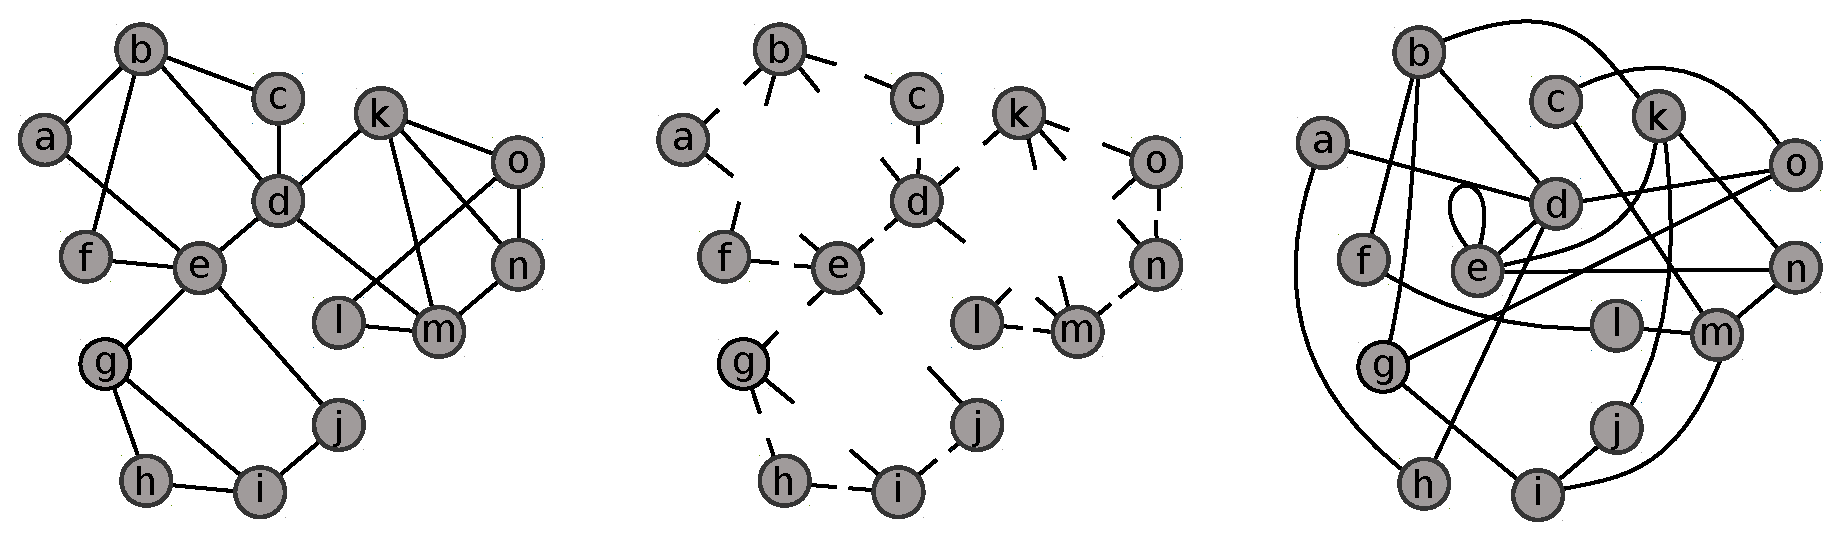
\includegraphics[width=0.8\linewidth]{img/ExpectedNodes/Example/modele_configuration.eps}
\caption{Exemple d'une génération du modèle de configuration avec à gauche le graphe initial, au milieu la mise en avant des demi-liens et à droite une génération aléatoire du modèle de configuration}
\label{fig:exemple_modele_configuration}
\end{figure}


Un n\oe{}ud est interne à $L$ si au moins un de ses liens appartient à $L$.
Ainsi pour calculer la probabilité qu'un n\oe{}ud soit interne dans le modèle de configuration, il faut donc calculer la probabilité qu'au moins un de ses demi-liens soit choisi lors du tirage aléatoire et sans remise de $2|L|$ demi-liens parmi les $2|E|$ demi-liens du graphe.
Soit $B_u$ la variable aléatoire correspondant au nombre de fois où le n\oe{}ud $u$ est tiré.
Cette variable suit une loi hypergéométrique $B_u \sim \mathcal{G}\left(2|E|,d_G(u),2m\right)$.
Avec cette notation, on définie $\mu_G$ de la manière suivante:

\begin{equation}
\label{eq:nbsommet_esp} \mu_{G}(|L|) = \sum_{u\in V} \mathbb{P}( B_u \geq 1 )
=  \sum_{u \in V} 1 - \dfrac{ \binom{2|E|-d(u)}{2|L|} }{ \binom{2|E|}{2|L|} }. 
\end{equation}

Voici quelques propriétés de la fonction $\mu_{G}(|L|)$ :
\begin{itemize}
\item La fonction $\mu_{G}$ dépend uniquement de la séquence de degrés $\{d_G(v)\}_{v \in V}$ et du nombre de liens.
%On peut montrer que cette fonction est Schur-concave, ainsi plus les degrés sont uniformément répartis plus il sera surprenant d'observer un groupe de liens correspondant à peu de n\oe{}uds.
\item Pour une distribution de degrés donnée, la fonction $\mu_{G}(|L|)$ est une fonction croissante de $|E|$.
\item Si $L=E$, alors le nombre de n\oe{}uds attendus est bien égal à $|V|$.
\item On a $\mu_{G}(1)\leq 2$, en effet le modèle nul n'interdit pas la présence de boucle.
\end{itemize}

Avec $\mu_G$, nous pouvons définir la qualité \emph{interne}, $Q_{in}$ d'un groupe de liens $L$:
  
\begin{equation}
\label{eq:qin} Q_{in}(L) = \dfrac{\mu_{G}(|L|) - |V_{in}(L)|}{\mu_{G}(|L|)}.
\end{equation}

Avec cette formulation, pour un groupe de taille $|L|$, plus le nombre de n\oe{}uds internes est faible, plus $Q_{in}$ sera élevée.

$Q_{in}$ permet d'évaluer la qualité interne d'un groupe mais il faut aussi tenir compte du voisinage.
En effet, observer une clique a l'intérieur d'une autre clique n'est absolument pas surprenant.
C'est pourquoi nous définissons également une qualité externe.
Le but est d'évaluer comment sont répartis les liens et n\oe{}uds adjacents.
Pour ce faire, nous allons également comparer le nombre de n\oe{}uds adjacents observé au nombre attendu dans le modèle de configuration.
Cependant à l'inverse de la qualité interne, la qualité externe est \textbf{mauvaise} si jamais le nombre de n\oe{}uds adjacent est plus faible qu'attendu.
En effet, s'il y a beaucoup de liens adjacents pour peu de n\oe{}uds, alors cela indique que le voisinage du groupe est dense et devrait être inclus dans le groupe.
Le cas idéal est que chaque lien adjacent soit relié à un n\oe{}ud différent.

Pour un n\oe{}ud interne $u$, soit $\bar{d}(L,u) = \sum_{v \in V} \mathbf{1}_{(u,v) \in E \setminus L}$ le degré de $u$ limité aux liens adjacents et $\bar{d}(L)=\sum_{u \in V_{in}(L)} \bar{d}(L,u)$.
L'espérance du nombre de n\oe{}uds adjacents est calculé comme le nombre de n\oe{}uds tirés lorsque $\bar{d}(L)$ demi-liens sont choisis aléatoirement et sans remise dans le modèle de configuration où les liens de $L$ ont été préalablement retirés.
Ce graphe aléatoire a la distribution de degrés suivante: $\{d_{G \setminus L }(u)\}_{u \in V}$ où $G \setminus L = (V,E\setminus L)$.
Dans ce cas, on ne tire pas aléatoirement un lien mais uniquement un demi-lien car l'autre demi-lien est un des demi-liens reliés aux n\oe{}uds internes.
L'espérance du nombre de n\oe{}uds adjacents se définit de la manière suivante:

\begin{equation}
	\mathbb{E}[\bar{d}(L)] = \mu_{G\setminus L}(\bar{d(L)}/2).
\end{equation}

Une illustration de ce processus est présentée dans la figure~\ref{fig:retourt_ext}.
Sur cette illustration, le groupe $L$ a un très mauvais voisinage et cela se reflète par un nombre de n\oe{}uds adjacents observés plus faible qu'attendu.
En particulier, ce sont les liens adjacents reliant deux n\oe{}uds internes qui pénalisent l'évaluation car ils comptent chacun pour deux demi-liens adjacents.

\begin{figure}
\centering
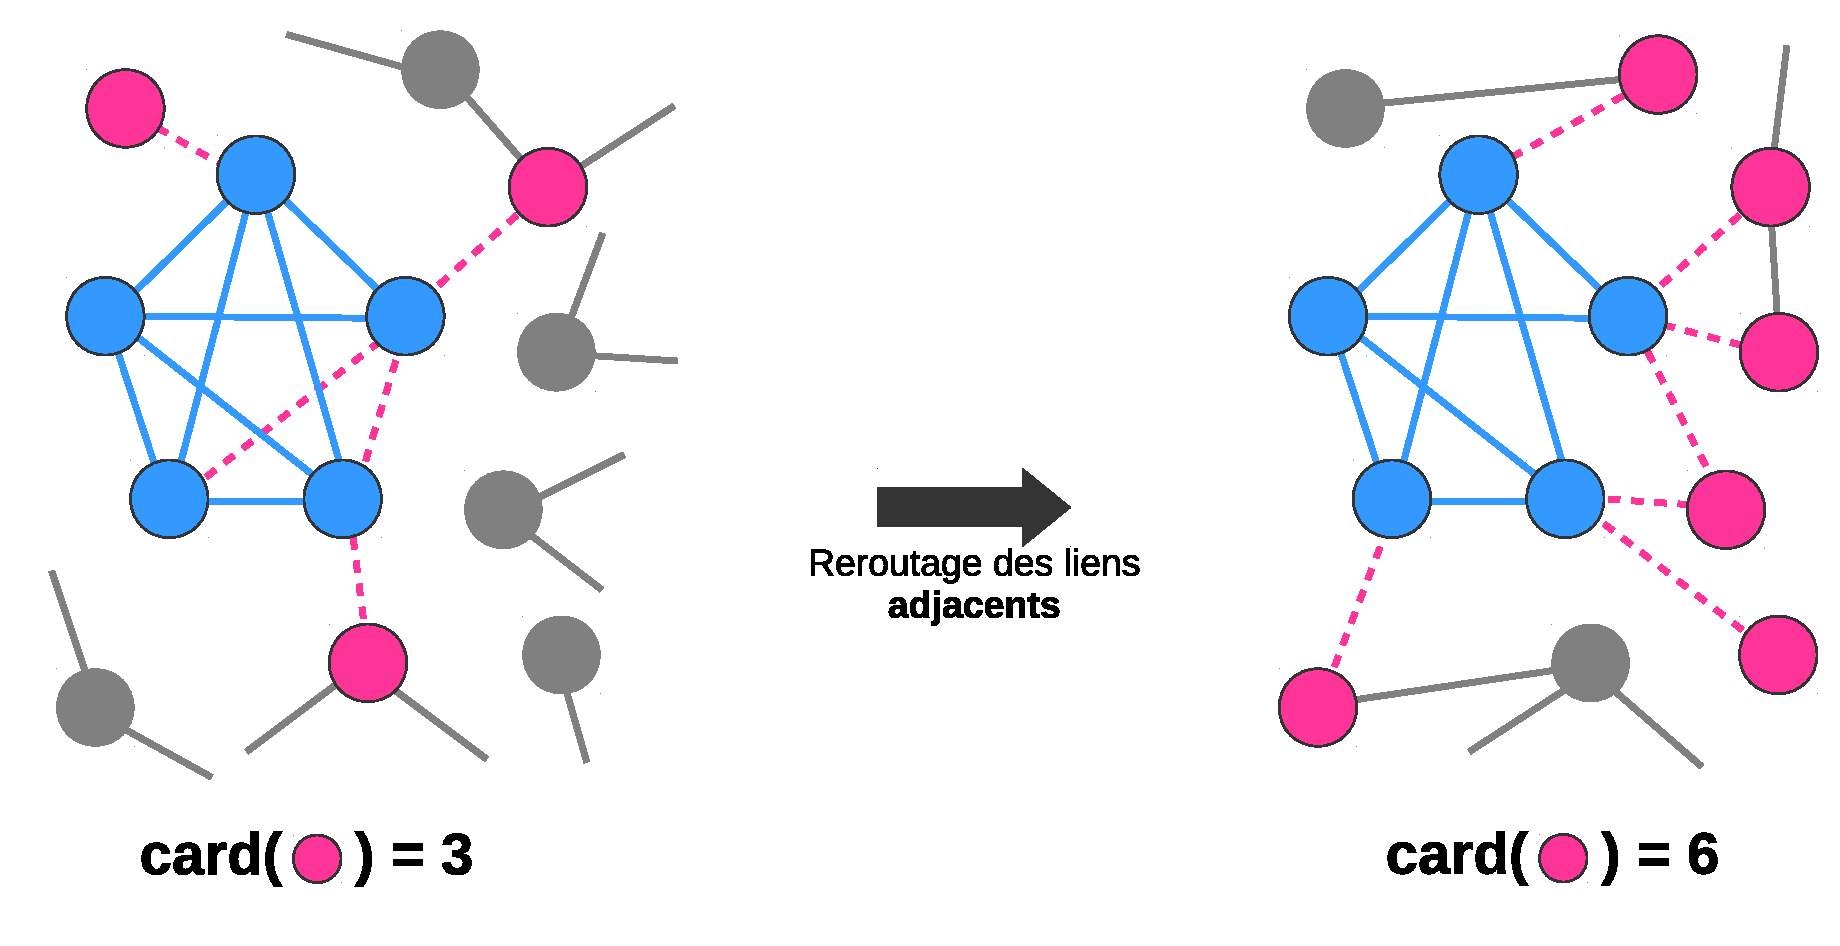
\includegraphics[width=0.7\linewidth]{img/ExpectedNodes/reroutageExt3}
\caption{Groupe de liens $L$ en \textcolor{semilightblue}{\textbf{bleu}} et ces liens adjacents en \textcolor{pinkyred}{\textbf{rose}} pointillés dans le graphe initial à gauche.
\`A droite, une réalisation du modèle de configuration où $L$ a été figé.}
\label{fig:retourt_ext}
\end{figure}

Comme il est intéressant de pénaliser les groupes ayant de mauvais voisinages mais qu'un bon voisinage n'est pas suffisant pour définir une bonne communauté, nous bornons à $0$ la qualité externe:

\begin{equation}
\label{eq:qext} Q_{ext}(L) = min \left(0, \dfrac{|V_{out}(L)| - \mu_{G\setminus L}(\bar{d}(L)/2)}{\mu_{G\setminus L}(\bar{d}(L)/2)} \right).
\end{equation}


Enfin, nous définissons \emph{Expected Nodes} pour un groupe $L$:
\begin{equation}
	\label{eq:qAlg}
	Q(L)  =  2\dfrac{ |L|Q_{in}(L) + |L_{out}|Q_{ext}(L)}{|L|+|L_{out}|}.
\end{equation}

La qualité interne est due aux liens de $L$ et la qualité externe aux liens adjacents.
C'est pourquoi nous pondérons $Q_{in}$ par $|L|$ et $Q_{ext}$ par $|L_{out}|$.



Nous détaillons maintenant certaines propriétés des formules \ref{eq:qext} et \ref{eq:qAlg} découlant des propriétés de $\mu_{G}$ en nous appuyant sur des exemples.
En s'intéressant aux n\oe{}uds adjacents $V_{out}$, on pénalise la présence de liens adjacents entre deux n\oe{}uds internes et la présence de n\oe{}uds adjacents fortement connectés avec les n\oe{}uds internes à $L$.
Prenons le cas extrême où $L$ est une clique qui est incluse dans une plus grande clique alors que le reste du graphe est quelconque.
Dans cette situation, $Q_{in}(L)$ est maximum car le groupe est une clique.
En revanche, $Q_{ext}(L)$ va fortement pénaliser la qualité du groupe car il y a dans ce cas beaucoup de liens adjacents pour très peu de n\oe{}uds adjacents.
Ainsi, la $Q_{ext}$ permet de pénaliser les n\oe{}uds adjacents ayant beaucoup de liens avec $L$.
L'idée est que ces liens adjacents devraient être intégrés à $L$.

Bien évidement, la solution n'est pas de systématiquement intégrer les liens adjacents car intégrer un lien adjacent peut également faire baisser $Q_{in}$.
Par exemple, un lien reliant deux groupes denses disjoints peut avoir une qualité positive.
Cette situation est visible dans la figure~\ref{fig:Partition_Couverture} partie gauche.
Ce lien tout seul a d'une part une qualité interne positive car $\mu_G(1) \leq 2$ et d'autre part il a une qualité externe nulle car chaque n\oe{}ud adjacent n'est relié qu'à un seul lien adjacent ce qui est le cas idéal.
Dans une situation plus générale, la qualité d'un lien isolé dépend du nombre de triangles dans lequel il se trouve.
Moins le nombre de triangles est élevé, meilleure sera la qualité externe.

Enfin il est intéressant de noter que la qualité du groupe contenant tous les liens est nulle.
En effet comme dit précédemment, $Q_{in}(E)$ est égal à zéro, voir l'équation \ref{eq:nbsommet_esp}.
De plus, si le groupe contient tous les liens alors il n'y a plus de liens adjacents et donc seule $Q_{in}(E)$ influe sur $Q(E)$.



Nous définissons \emph{Expected Nodes} pour une partition de liens $\mathcal{L}$ comme la moyenne pondérée de la qualité de chaque groupe:
\begin{equation}
\label{eq:qualite_globale} Q_G(\mathcal{L}) = \dfrac{\sum_{L\in \mathcal{L}} |L|Q(L)}{|E|}.
\end{equation}

D'autres choix de pondération pour $Q_{in}$, $Q_{ext}$ et $Q_G$ ont été testés en utilisant le nombre de n\oe{}uds au lieu du nombre de liens mais elles ont été abandonnées lors des tests qui sont présentés dans la section~\ref{sec:expected_comp}.

\section{Comparaison}
\label{sec:expected_comp}
Nous évaluons maintenant \emph{Expected Nodes} en utilisant trois jeux de test.
Sur ces jeux de test, nous appliquons également des fonctions de qualités reconnues:
\emph{Partition Density}~\cite{Ahn2010a} et les fonctions de qualité proposées par Evans et Lambiotte~\cite{Evans2009} que nous nommons $Evans1$, $Evans2$ et $Evans3$.
Pour chaque graphe de test, nous créons empiriquement plusieurs partitions de liens et nous évaluons chaque partition avec toutes les fonctions de qualité.

\subsection{Cas du graphe complet}
\label{Completegraph}
Le premier jeu de test est assez simple puisqu'il s'agit d'un graphe complet.
Le but est de vérifier que \emph{Expected Nodes} n'a pas un comportement dégénéré.
Nous étudions un graphe complet de $100$ n\oe{}uds\,\footnote{Nous avons obtenu des résultats similaires pour un graphe de $500$ n\oe{}uds.}.
Sur ce graphe, nous définissons plusieurs partitions.
La première est la partition triviale où tous les liens sont dans un unique groupe.
Nous définissons également deux familles de partitions: une séparant les liens en deux groupes et une séparant les liens en 3 groupes.
Soit $V'$ un ensemble de $p$ n\oe{}uds où $p$ est un paramètre $p<|V|$.
Les deux familles de partitions placent les liens de $V' \times V'$ dans un groupe.
Pour la partition en 2 groupes, tous les autres liens sont mis dans un second groupe.
Pour la partition en 3 groupes, les liens de $V' \times V\setminus V'$ sont dans un second groupe et les liens de $V \setminus V' \times V\setminus V'$ sont dans un troisième.
Ces répartitions sont illustrées dans la figure~\ref{fig:1C}.

\begin{figure}
\centering
	\begin{subfigure}{0.2\linewidth}
		\includegraphics[width=\linewidth]{img/ExpectedNodes/1Clique/Clique2}
		\caption{\label{fig:1C2}}	
	\end{subfigure}	\hspace{2cm}
	\begin{subfigure}{0.2\linewidth}
			\includegraphics[width=\linewidth]{img/ExpectedNodes/1Clique/Clique3}
			\caption{\label{fig:1C3}}		
	\end{subfigure}
	\caption{Deux partitions de liens pour un graphe complet à $10$ n\oe{}uds avec $p=5$: (A) partition en deux groupes et (B) partition en trois groupes.
	Les n\oe{}uds noirs sont les n\oe{}uds appartenant à $V'$ et la couleur d'un lien correspond à son groupe.}
	\label{fig:1C}
\end{figure}


Comme le graphe est complet, la meilleure solution est d'avoir un seul groupe contenant l'ensemble des liens, \emph{i.e.} la partition triviale devrait avoir une meilleure évaluation que les autres partitions.
La figure~\ref{fig:1Cres} présente les résultats.
Pour chaque valeur de $p$ et chaque fonction de qualité, nous calculons les évaluations des partitions en deux et en trois groupes ainsi que l'évaluation de la partition triviale.
L'évaluation de la partition triviale n'est pas dépendante de $p$ et n'est calculée qu'une seule fois.
Tout d'abord, la construction de cet exemple est symétrique pour les partitions en trois groupes.
En effet, la partition en trois groupes lorsque $p$ est égal à $24$ est complètement équivalente à la partition en deux groupes lorsque $p$ est égal à $76$.
Pour les partition en deux groupes, ces deux situations diffèrent par liens de $V' \times V\setminus V'$.
Par ailleurs, il est possible de définir formellement la qualité de chacune de ces partitions selon toutes les fonctions de qualité.
Cependant, la complexité des équations, surtout pour \emph{Expected Nodes} et $Evans_x$, rend le résultat difficilement interprétable.


De manière assez surprenante, les fonctions $Evans1$ et $Evans2$ ne passent pas ce test car elles évaluent la partition en deux ou trois groupes comme meilleure que la partition triviale.
Selon la \emph{Partition Density}, \emph{Expected Nodes} et $Evans3$, la partition triviale est la meilleure des partitions.
La fonction $Evans3$ diffère légèrement des deux autres car elle a une amplitude plus faible ($\approx 10^{-3}$).

%\begin{equation}
%Expected\_nodes(p) = \dfrac{1}{C(100)}(C(p) Q(L_{gauche}) + C(100-p) Q(L_{droite}))
%\end{equation}
%\begin{equation}
%Q(L_{gauche})= 2\dfrac{C(p) 100 (1 - \dfrac{ \binom{2C(100) - 99}{2C(p)} }{ \binom{2C(100)}{2C(p)} }) - (100-p)p }{C(p)+ (100-p)p}
%\end{equation}
%$C(p)= \dfrac{p(p-1)}{2}$

\begin{figure}[h]
\centering
	\begin{subfigure}{0.35\linewidth}
		\includegraphics[width=\linewidth]{img/ExpectedNodes/1Clique/Clique_Partitiondensity.eps}
		\caption{\label{fig:1CAhn}\emph{Partition Density}}		
	\end{subfigure}\hspace*{1cm}
	\begin{subfigure}{0.35\linewidth}
		\includegraphics[width=\linewidth]{img/ExpectedNodes/1Clique/Clique_Evans1.eps}
		\caption{\label{fig:1CE2}\emph{Evans1, Evans2}}		
	\end{subfigure}

	\begin{subfigure}{0.35\linewidth}
		\includegraphics[width=\linewidth]{img/ExpectedNodes/1Clique/Clique_Evans3.eps}
		\caption{\label{fig:1CE3}\emph{Evans3}}		
	\end{subfigure}\hspace*{1cm}
	\begin{subfigure}{0.35\linewidth}
		\includegraphics[width=\linewidth]{img/ExpectedNodes/1Clique/Clique_Expectednode.eps}
		\caption{\label{fig:1CMod}\emph{Expected Nodes}}		
	\end{subfigure}
		
		\caption{\'Evaluation des 5 fonctions de qualité sur un graphe complet de $100$ n\oe{}uds pour trois type de partitions.
		Les partitions testées sont présentées dans la section~\ref{Completegraph}.
		Par définition, les résultats pour $Evans1$ et $Evans2$ sont identiques.
		Les lignes en gris, pointillées et noires représentent respectivement la partition triviale, les partitions en deux groupes et les partitions en trois groupes.}
		\label{fig:1Cres}
\end{figure}

\subsection{Cas de deux cliques chevauchantes}
\label{subsec:2cliques}

Le second jeu de test est un peu plus évolué puisqu'il s'agit deux cliques de $100$ n\oe{}uds chacune se chevauchant plus ou moins fortement.
Ainsi, nous générons les graphes en fonction du nombre de n\oe{}uds appartenant aux deux cliques.
Sur chaque graphe, nous définissons également plusieurs partitions.
La première est la partition triviale où tous les liens sont dans un unique groupe.
Nous définissons également cinq autres partitions qui contiennent 2, 3 ou 5 groupes.
Soit $V_1$ l'ensemble des n\oe{}uds de la première clique, $V_2$ celui de la deuxième clique et $V_{12}=V_1 \cap V_2$ l'ensemble de n\oe{}uds commun à $V_1$ et $V_2$.
Cette taxonomie des n\oe{}uds est illustrée dans la figure~\ref{fig:2Ctaxo}.

Par abus de notations, nous notons également $V_{11}=V_1\setminus V_2$ et $V_{22}=V_2\setminus V_1$.
Il y a deux partitions en deux groupes: la partition $2A$ et $2B$.
Dans la partition $2A$, les liens entre les n\oe{}uds de $V_{22}$ forment un groupe alors que le reste des liens forme l'autre groupe.
Dans la partition $2B$, les liens entre les n\oe{}uds de $V_{1}$ forment un groupe alors que le reste des liens forme l'autre groupe.

Il y a également deux partitions en trois groupes: la partition $3A$ et $3B$.
Dans la partition $3A$, les liens entre les n\oe{}uds de $V_{12}$ forment un premier groupe et les liens appartenant à $V_1\times V_{11}$ (resp. $V_2\times V_{22}$) forment un deuxième (resp. troisième) groupe.
Dans la partition $3B$, les liens entre les n\oe{}uds de $V_{11}$ (resp. $V_{22}$) forment un premier (resp. deuxième) groupe alors que le reste des liens forme un troisième groupe.

Enfin dans la partition $5$ en cinq groupes, il existe 3 groupes correspondant aux liens entre les n\oe{}uds de respectivement $V_{11}$, $V_{12}$ et $V_{22}$.
Il y a également un groupe pour les liens appartenant à $V_{11} \times V_{12}$ et un autre pour ceux appartenant à $V_{12} \times V_{22}$.

Ces partitions sont illustrées dans la figure~\ref{fig:2C}.

\begin{figure}[h]
\centering
	\begin{subfigure}[b]{0.3\linewidth}
		\includegraphics[width=\linewidth]{img/ExpectedNodes/2Cliques/PartitionExamples/Clique2A}
		\caption{2A\label{fig:2C2A}}	
	\end{subfigure}	
	\begin{subfigure}[b]{0.3\linewidth}
		\includegraphics[width=\linewidth]{img/ExpectedNodes/2Cliques/PartitionExamples/Clique2}
		\caption{Taxonomie\label{fig:2Ctaxo}}	
	\end{subfigure}	
	\begin{subfigure}[b]{0.3\linewidth}
			\includegraphics[width=\linewidth]{img/ExpectedNodes/2Cliques/PartitionExamples/Clique2B}
			\caption{2B\label{fig:2C2B}}		
	\end{subfigure}

	\begin{subfigure}{0.3\linewidth}
			\includegraphics[width=\linewidth]{img/ExpectedNodes/2Cliques/PartitionExamples/Clique3A}
			\caption{3A\label{fig:2C3A}}		
	\end{subfigure}
	\begin{subfigure}{0.3\linewidth}
		\includegraphics[width=\linewidth]{img/ExpectedNodes/2Cliques/PartitionExamples/Clique3B}
		\caption{3B\label{fig:2C3B}}	
	\end{subfigure}
	\begin{subfigure}{0.3\linewidth}
			\includegraphics[width=\linewidth]{img/ExpectedNodes/2Cliques/PartitionExamples/Clique5}
			\caption{5\label{fig:2C5}}		
	\end{subfigure}
	\caption{Différentes partitions d'un graphe constitué de deux cliques de $9$ se chevauchant sur $3$ n\oe{}uds.
	En (B), taxonomie des n\oe{}uds du graphe.
	En (A) et (C), deux partitions en deux groupes.
	En (D) et (E), deux partitions en trois groupes.
	En (F), une partition en cinq groupes.
	La couleur d'un lien correspond à son groupe.}
	\label{fig:2C}
\end{figure}

Pour chaque graphe en fonction du chevauchement $p$, nous évaluons ces cinq partitions mais aussi la partition $LC$ trouvée par \emph{link clustering}~\cite{Ahn2010a} et les partitions $EX$ trouvées par les méthodes de Evans et Lambiotte~\cite{Evans2009}.
Ces algorithmes optimisent respectivement \emph{Parition Density}, \emph{Evans1}, \emph{Evans2} et \emph{Evans3}.
Ces partitions sont ensuite évaluées par les fonctions de qualité \emph{Partition Density}, $Evans1$, $Evans2$, $Evans3$ et \emph{Expected Node}.
La figure~\ref{fig:2Cres} présente les résultats.


\begin{figure}[h]
\centering
	\begin{subfigure}{0.31\textwidth}
		\includegraphics[width=\linewidth]{img/ExpectedNodes/2Cliques/2Clique_Partition_density.eps}
		\caption{\label{fig:2CAhn}Partition density}		
	\end{subfigure}
	\begin{subfigure}{0.31\textwidth}
		\includegraphics[width=\linewidth]{img/ExpectedNodes/2Cliques/2Clique_Expected_Nodes.eps}
		\caption{\label{fig:2CMod}Expected Nodes}		
	\end{subfigure}
	\begin{subfigure}{0.07\textwidth}
		\includegraphics[width=\linewidth]{img/ExpectedNodes/2Cliques/legend.eps}
	\end{subfigure}
	
	\begin{subfigure}{0.31\textwidth}
		\includegraphics[width=\linewidth]{img/ExpectedNodes/2Cliques/2Clique_Evans1.eps}
		\caption{\label{fig:2CE1}Evans1}		
	\end{subfigure}
	\begin{subfigure}{0.31\textwidth}
		\includegraphics[width=\linewidth]{img/ExpectedNodes/2Cliques/2Clique_Evans2.eps}
		\caption{\label{fig:2CE2}Evans2}		
	\end{subfigure}
	\begin{subfigure}{0.31\textwidth}
		\includegraphics[width=\linewidth]{img/ExpectedNodes/2Cliques/2Clique_Evans3.eps}
		\caption{\label{fig:2CE3}Evans3}		
	\end{subfigure}
	\caption{\'Evaluation des cinq fonctions de qualité sur un graphe composé de deux cliques de $100$ n\oe{}uds se chevauchant sur $p$ n\oe{}uds pour dix partitions différentes.
	Les partitions testées sont présentées dans la section~\ref{subsec:2cliques}.
	Les lignes en trait plein et pointillé représentent respectivement les partitions fixées arbitrairement et les partitions trouvées empiriquement.}
	\label{fig:2Cres}
\end{figure}

Comme le graphe étudié est composé de deux cliques se chevauchant de plus en plus, il n'y a pas une seule vérité de terrain.
Lorsque le chevauchement est faible, les partitions $2B$ et $3A$ devraient avoir les meilleures évaluations.
Lorsque le chevauchement est plus important, c'est la partition $1$ en une seule communauté qui devrait avoir la meilleure évaluation.

Dans le cas de $EvansX$, ce sont les partitions $EX$ qui obtiennent les meilleures évaluations, en particulier pour $Evans1$ et $Evans2$.
L'optimisation de ces fonctions de qualité mène donc à trouver des partitions qui ont une qualité plus élevée que la vérité de terrain mais qui sont différentes.
Ces fonctions de qualités ne sont donc pas à même de capturer une vérité de terrain comme la meilleure partition.
Il est toutefois important de noter que dans le cas de $Evans3$, la différence entre $E3$ et $2B$ reste faible.

Pour les fonctions de qualité \emph{Partition density} et \emph{Expected Nodes}, c'est bien la partition $2B$ qui obtient le meilleur score lorsque le chevauchement est faible.
Lorsque le chevauchement est plus important, c'est la partition $1$ qui obtient la meilleure évaluation.
La principale différence entre ces deux fonctions de qualité est la proportion de chevauchement à partir duquel la meilleure partition change.
Dans le cas de \emph{Partition density}, ce changement intervient lorsque le chevauchement dépasse $40$ n\oe{}uds.
Pour \emph{Expected Nodes}, ce changement intervient lorsque le chevauchement dépasse $30$ n\oe{}uds.

\subsection{Graphe LF}
Nous utilisons maintenant un jeu de test plus évolué.
Il n'existe pas à notre connaissance de générateur de graphe aléatoire avec une structure communautaire sur les liens.
Nous utilisons donc le générateur proposé par Lancichinetti et Fortunato~\cite{Lancichinetti2009b}.
Ce générateur aléatoire permet de générer des graphes ayant une structure communautaire chevauchante sur les n\oe{}uds.
Comme nous voulons évaluer une partition de liens, il est nécessaire de transformer cette vérité de terrain.
Nous introduisons deux transformations de la couverture des n\oe{}uds en deux partitions de liens, $TA$ et $TB$, voir figure~\ref{fig:Trans}.


Reprenons l'exemple d'un réseau d'interactions de personnes où chaque personne appartient à différents groupes.
Afin de simplifier l'exemple, nous considérons qu'il n'existe que deux groupes: \emph{travail} et \emph{amis}.
Le but est de déterminer le type d'une interaction à partir des groupes des personnes.

Si deux personnes partagent un seul groupe, par exemple \emph{travail}, alors il est clair que l'interaction entre ces deux personnes devraient également être de type \emph{travail}.

Si deux personnes ne partagent aucune communauté, l'une est dans \emph{travail} et l'autre dans \emph{amis}, alors plusieurs choix sont possible pour le type de l'interaction.
Soit l'interaction a un type \emph{travail-amis} car on considère que toutes les interactions reliant deux personnes des groupes \emph{travail} et \emph{amis} sont de même types.
Soit l'interaction a son propre type car on considère qu'elle est unique.

Enfin, deux personnes peuvent partager plus qu'une communauté si les deux sont dans les communautés \emph{travail} et \emph{amis}.
Dans ce cas, l'interaction peut être due à l'un de ces deux groupes indépendamment.

Nous définissons maintenant de manière plus formelle cette transformation qui est illustrée dans la figure~\ref{fig:Trans}.
Soit $u,v \in V$, $C_{u,v}$ désigne l'intersection des communautés de $u$ et $v$ dans la couverture et $U_{u,v}$ désigne leur union.
Nous définissons le groupe d'un lien $(u,v) \in E$ dans $TA$ et $TB$ de la manière suivante:
\begin{description}
\item[\textbf{intra-communauté}] si $|C_{u,v}| = 1$ alors $(u,v)$ est dans la communauté $C_{u,v}$;
\item[\textbf{inter-communauté}] si $|C_{u,v}| = 0$ alors dans $TA$, $(u,v)$ appartient à sa propre communauté.
Dans $TB$, le lien appartient à la communauté $U_{u,v}$, qui contient l'ensemble des liens $(u',v')$ tel que $U_{u',v'}=U_{u,v}$;
\item[\textbf{chevauchant}] si $|C_{u,v}| > 1$ alors le lien $(u,v)$ appartient aléatoirement à une des communautés appartenant à $C_{u,v}$.
\end{description}

\begin{figure}
\centering
\includegraphics[width=0.9\linewidth]{img/ExpectedNodes/Example/GroundTruthTransformation}
\caption{Construction de $TA$ et $TB$ depuis une couverture de n\oe{}uds.
La couleur des liens indique leur groupe.}
\label{fig:Trans}
\end{figure}

Pour générer le graphe, nous avons appliqué un jeu de paramètres classiquement utilisé dans la littérature~\cite{Fortunato2010}.
Ainsi, nous avons généré des graphes de $500$ n\oe{}uds ayant un degré moyen de $25$, un degré max de $50$ et $10$ n\oe{}uds appartenant à deux communautés et des communautés ayant une taille comprise entre $20$ et $100$.
Le degré est tiré selon une loi exponentielle de paramètre $-2$ et la taille des communautés a $-1$ comme paramètre.
Enfin, 90\% des liens sont à l'intérieur d'une communauté et les 10\% restant sont répartis de manière aléatoire.
Avec ces paramètres, il y a en moyenne $5620$ liens intra-communauté, $625$ liens inter-communauté et seulement $5$ liens chevauchants.

Pour chaque graphe généré, nous testons les partitions $TA$ et $TB$ mais aussi la partition $LC$ trouvée par \emph{link clustering}~\cite{Ahn2010a} et les partitions $EX$ trouvées par les méthodes de Evans et Lambiotte~\cite{Evans2009}.
Ces partitions sont ensuite évaluées par les fonctions de qualité \emph{Partition Density}, $Evans1$, $Evans2$, $Evans3$ et \emph{Expected Node}.
Une illustration d'un graphe généré et des exemples de groupes capturés par $LC$ et $E2$ sont présentés dans la figure~\ref{fig:LFR_Exemple}.

\begin{figure}
\centering
	\begin{subfigure}{0.31\textwidth}
		\includegraphics[width=\linewidth]{img/ExpectedNodes/LF/Graphe_Complet_select.png}
		\caption{}
	\end{subfigure}
	\begin{subfigure}{0.31\textwidth}
		\includegraphics[width=\linewidth]{img/ExpectedNodes/LF/E2_bis.png}
		\caption{}
		\label{fig:LFR_ExempleE2}
	\end{subfigure}
	\begin{subfigure}{0.31\textwidth}
		\includegraphics[width=\linewidth]{img/ExpectedNodes/LF/Ahn.png}
		\caption{}
		\label{fig:LFR_ExempleLC}	
	\end{subfigure}

	\caption{Exemple de graphe généré par le LF en (A) avec une communauté de liens intra-communauté de la vérité de terrain mise en avant en vert.
	En (B) zoom sur le groupe le plus proche dans $E2$ dont les liens sont en verts.
	En (C) zoom sur le groupe le plus proche dans $LC$ dont les liens sont en verts.
	Dans la figure (C), les liens de la communauté de la vérité de terrain sont en gris. }
	\label{fig:LFR_Exemple}
\end{figure}


Dans $LC$, $TA$, $TB$, il y a $720$, $650$, $70$ groupes en moyenne.
Dans $E1$, $E2$ et $E3$, il n'y a que $11$ groupes en moyenne.
Afin d'observer la ressemblance de ces partitions, nous avons utilisé la NMI~\cite{Danon2005}.
Il apparaît que les partitions $TA$ et $TB$ sont les deux partitions les plus proches l'une de l'autre.
Nous remarquons que les partitions $E1$, $E2$ et $E3$ sont similaires.
Ensuite, nous remarquons que les partitions $EX$ diffèrent de $TA$ et de $TB$ uniquement sur les liens inter-communautés.
En effet s'ils ne sont pas pris en compte lors de la comparaison, alors $EX$, $TA$ et $TB$ sont identiques.
Il semble en effet que les liens inter-communautés soient arbitrairement distribués entre les plus grosses communautés adjacentes pour les partitions $EX$, ce qui est visible dans la figure~\ref{fig:LFR_ExempleE2}.
Enfin, la partition $LC$, bien que proche de $TA$ et $TB$, est un peu plus différente.
Ses $720$ groupes semblent plus petits mais aussi plus denses que ceux de $TA$ ou $TB$.
En particulier, les liens intra-communautés peuvent être séparés en plusieurs groupes, comme dans la figure~\ref{fig:LFR_ExempleLC}.
Les quatre partitions sont donc différentes et mettent en avant différentes caractéristiques.

Nous procédons maintenant à l'évaluation de ces partitions par les fonctions de qualité.
Comme la génération de graphes est aléatoire, les évaluations présentées dans la figure~\ref{fig:LF} représentent $30$ générations.
On remarque tout d'abord que ni $TA$ ni $TB$ n'a la meilleure évaluation selon $EvansX$ (figures~\ref{fig:LFE1} à ~\ref{fig:LFE3}) ou \emph{Partition Density} (figure~\ref{fig:LFAhn}) même si $TA$ et $TB$ représentent nos vérités de terrain.
Dans le cas de $EvansX$, ce sont les partitions $EX$ qui obtiennent les meilleures évaluations.
Cela prouve l'efficacité de l'algorithme pour optimiser $EvansX$ mais remet en cause la pertinence des critères $EX$ pour mettre en avant la vérité de terrain.
Notre fonction \emph{Expected Nodes} se comporte différemment des 4 autres.
Tout d'abord, c'est la vérité de terrain $TA$ qui obtient la meilleure évaluation puis il s'agit de $TB$ ou $LC$ selon les générations.
Notre mesure semble donc bien mettre en avant la vérité de terrain générée.
De plus, \emph{Expected Nodes} évalue différemment les partitions $TA$ et $TB$ contrairement à \emph{Partition Density} et \emph{EvansX}.
C'est un point important car, dans la partition $TB$, les liens inter-communautés peuvent donner lieu à des groupes non-connexes dans $TB$, voir figure~\ref{fig:Trans}.
Ce phénomène est très pénalisé par \emph{Expected Nodes}.
Enfin selon \emph{Expected Nodes}, les partitions $EX$ ont une faible qualité et cela est également dû aux liens inter-communautés.
En effet en étant intégrés à une communauté adjacente, ils augmentent fortement le nombre de n\oe{}uds internes ce qui fait baisser $Q_{in}$.

Avec ce test, nous mettons en évidence les limites des fonctions de qualité existantes.
Les fonctions de qualité $EvansX$ ne peuvent pas permettre de capturer les vérités de terrain générées par LF.
En effet, l'algorithme de Louvain est capable de trouver des partitions ayant une évaluation plus élevée que la vérité de terrain.
La \emph{Partition Density}, quant à elle, souffre surtout de son incapacité à différencier clairement des partitions différentes.
Cela se matérialise par des évaluations très similaires pour les vérités de terrain et la partition $LC$.
Il en résulte que la \emph{Partition Density} ne semble pas à même de différencier clairement des partitions clairement non similaires.
Lors de ces tests, \emph{Expected Nodes} ne semble pas souffrir de ces défauts.
Pour ces raisons, nous pensons que \emph{Expected Nodes} est une mesure qui permet de bien évaluer les partitions de liens.

\begin{figure}
\centering
	\begin{subfigure}{0.31\textwidth}
		\includegraphics[width=\linewidth]{img/ExpectedNodes/LF/LFR1_Partitiondensity_ALL.eps}
		\caption{\label{fig:LFAhn}Partition density}		
	\end{subfigure}
	\begin{subfigure}{0.31\textwidth}
		\includegraphics[width=\linewidth]{img/ExpectedNodes/LF/LFR1_ExpectedNodes_ALL.eps}
		\caption{\label{fig:LFMod}Expected Nodes}		
	\end{subfigure}
	
	\begin{subfigure}{0.31\textwidth}
		\includegraphics[width=\linewidth]{img/ExpectedNodes/LF/LFR1_Evans1_ALL.eps}
		\caption{\label{fig:LFE1}Evans1}		
	\end{subfigure}
	\begin{subfigure}{0.31\textwidth}
		\includegraphics[width=\linewidth]{img/ExpectedNodes/LF/LFR1_Evans2_ALL.eps}
		\caption{\label{fig:LFE2}Evans2}		
	\end{subfigure}
	\begin{subfigure}{0.31\textwidth}
		\includegraphics[width=\linewidth]{img/ExpectedNodes/LF/LFR1_Evans3_ALL.eps}
		\caption{\label{fig:LFE3}Evans3}		
	\end{subfigure}
	\caption{Boites à moustaches des évaluations des cinq fonctions de qualité pour les différentes partitions de liens. 
	La boite représente le premier et troisième quartile ainsi que la médiane.
	Les moustaches s'étendent sur $1.5$ fois l'écart entre le premier et le troisième quartile. 
	Les croix sont les points au delà des moustaches.
	}
	\label{fig:LF}
\end{figure}


\section{Calcul et optimisation}
Jusqu'à maintenant, nous avons évalué \emph{Expected Nodes} sans nous attacher ni à son calcul ni à son optimisation.
Nous discutons maintenant de la complexité de calcul d'\emph{Expected Nodes} pour une partition donnée.
Le calcul de la qualité interne \ref{eq:qin} nécessite d'évaluer la probabilité qu'un n\oe{}ud soit tiré.
Ce calcul nécessite d'évaluer pour un n\oe{}ud $u$: $1 - \dfrac{ \binom{2|E|-d(u)}{2|L|} }{ \binom{2|E|}{2|L|} }$, ce qui peut être assez coûteux.
Ce calcul correspond à une loi hypergéométrique.
Or sous certaines conditions, une loi hypergéométrique peut être approché par une loi binomiale ce qui simplifie le calcul à: $1 - (1- \dfrac{|L|}{|E|})^{|L|}$ ce qui est plus rapide.
Lors de nos tests, le biais induit par cette approximation reste assez faible, de l'ordre de $0.01\%$ en moyenne.
Ce changement de calcul est équivalent à considérer un tirage avec remise au lieu de tirage sans remise.
De plus cette probabilité ne dépend que du degré du n\oe{}ud et du nombre de liens dans le groupe.
Donc, tous les n\oe{}uds ayant le même degré donnent lieu à la même probabilité.
Si l'on considère que l'évaluation de la probabilité pour un n\oe{}ud peut se faire en $O(1)$ alors, pour un groupe donné, il est possible de calculer sa qualité en $O(|\{d_G(v)\}_{v \in V}|)$.
Cette formulation est très efficace lorsque beaucoup de n\oe{}uds ont le même degré.
Enfin comme la qualité d'un groupe ne dépend que de sa taille, on peut calculer la qualité d'une partition $\mathcal{L}$ en $O(\{|L_i|\}_{L_i \in \mathcal{L}})$.

Il est donc assez rapide de calculer $Q_{in}$.
En revanche, la situation est complètement différente pour $Q_{ext}$.
Le processus de calcul est similaire.
On peut également appliquer l'approximation de la loi hypergéométrique par une loi binomiale mais deux n\oe{}uds de même degré ne vont plus forcément avoir la même probabilité d'être tirés.
En effet, $Q_{ext}$ n'utilise pas le graphe initial mais le graphe $G\setminus L_i$.
Pour chaque n\oe{}ud, il faut évaluer son degré dans ce nouveau graphe.
Le calcul de $Q_{ext}$ pour un groupe se fait donc en $O(n)$.
Pour l'évaluation d'une partition, il n'est pas non plus possible de considérer comme équivalents des groupes de même taille.
Le coût pour évaluer une partition est donc en $O(|\mathcal{L}|n)$.
Le code pour évaluer une partition de liens d'un graphe avec \emph{Expected Nodes} mais aussi avec \emph{Partition Density}, $Evans1$, $Evans2$ et $Evans3$ est disponible en ligne: \url{https://github.com/ksadorf/ExpectedNodes}.


Malgré ce coût élevé, nous avons développé un premier algorithme d'optimisation glouton de \emph{Expected Node}.
Le principe de fonctionnement est le suivant.
Chaque lien est initialement dans son propre groupe.
Puis à chaque itération, on considère deux types de modification de la solution courante: soit la meilleure fusion de deux communautés soit le meilleur changement de communauté d'un seul lien.
On fusionne ou change de communauté un lien si cela améliore la qualité de la partition.
Les fusions considérées sont les fusions entre des communautés adjacentes.
Les changement de liens se font également uniquement avec une communauté adjacente.
On continue de modifier la solution courante tant qu'elle est améliorable par un de ces mouvements.
Malheureusement cette approche souffre de deux problèmes majeurs.
Tout d'abord le calcul du gain est coûteux et rend impossible l'étude de grands jeux de données.
Ensuite dans nos tests dans les graphes générés par LF, il semble que cette méthode reste bloquée sur des optimum locaux bien plus faibles que la vérité de terrain, voir la figure~\ref{fig:LF_bis_EN} où la qualité de la partition trouvée par notre algorithme, notée $EN$, est présentée.
Il faudrait donc tester d'autres heuristiques d'optimisation mais aussi travailler sur une méthode de calcul du gain plus optimisée.

Malgré ces limitations, nous avons tout de même tiré parti de cet algorithme naïf afin de tester si une partition donnée peut être améliorée.
En effet même si l'algorithme n'est pas adapté pour trouver une partition ayant une qualité élevée en partant de zéro, il peut modifier une partition donnée pour l'améliorer. 
Nous avons donc utilisé les partitions $TA$ et $TB$ comme partition de départ de l'algorithme et nous avons observé si l'algorithme est capable d'améliorer les vérités de terrain.
Les changements qu'apportent notre algorithme se portent principalement sur les liens inter-communautés.
Dans le cas de $TA$, chaque lien inter-communauté constitue initialement une communauté.
Or, il se peut que plusieurs liens inter-communautés soient connectés aux même n\oe{}uds.
Dans ce genre de situation, notre algorithme fusionne ces liens dans une communauté augmentant légèrement la qualité globale.
Après optimisation, nous constatons que les partitions $TA$ et $TB$ peuvent être légèrement améliorées mais qu'elles sont très proches du maximum local lorsque l'on considère notre algorithme d'optimisation,
voir la figure~\ref{fig:LF_bis_EN} où les partitions $TA+$ et $TB+$ sont les versions améliorées de $TA$ et $TB$.
\begin{figure}
\centering
	\begin{subfigure}{0.31\textwidth}
		\includegraphics[width=\linewidth]{img/ExpectedNodes/LF/LFR1_Modified_ALL.eps}
	\end{subfigure}
	
	\caption{Boite à moustaches des évaluations selon \emph{Expected Nodes} pour différentes partitions.
	$TA$ et $TB$ sont les vérités de terrains, $EN$ est la partition trouvée par notre algorithme et enfin $TA+$ et $TB+$ sont les versions améliorées par notre algorithme de $TA$ et $TB$.
	}
	\label{fig:LF_bis_EN}
\end{figure}

\section{Conclusion}

Nous avons introduit de nouveaux critères pour l'évaluation des partitions de liens tenant compte de la répartition des n\oe{}uds internes et externes d'un groupe.
\`A partir de ces critères, nous avons défini une mesure de qualité, \emph{Expected Nodes}, basée sur la différence entre le nombre de n\oe{}uds induits par un groupe de liens et le nombre de n\oe{}uds attendu dans un modèle nul.
Cette approche est similaire à celle qui a donné lieu à la modularité.
En plus de s'inspirer de la modularité, \emph{Expected Nodes} ne prend pas uniquement en compte la répartition de ses n\oe{}uds induits mais également celle des n\oe{}uds et liens adjacents.
Ce changement permet d'avoir une évaluation plus fine d'une communauté.
Pour montrer la pertinence de cette nouvelle fonction de qualité, nous évaluons quatre fonctions de qualité de la littérature.
Nous montrons que, sur nos jeux de tests, \emph{Expected Nodes} semble être la plus à même de capturer la vérité de terrain et de différencier des partitions différentes.
Malgré le coût de calcul élevé d'\emph{Expected Nodes}, nous avons implémenté un premier algorithme d'optimisation agglomératif.
Cet algorithme n'est, pour l'instant, pas capable d'obtenir des partitions avec des scores élevés.
Cependant il nous a permis de vérifier que les vérités de terrain générées par LF sont des quasi-optimum locaux selon \emph{Expected Nodes}.
Bien qu'il soit possible d'améliorer légèrement les vérités de terrain, la structure de l'optimum local est très proche de la partition initiale.


\subsection{Perspectives}

Les perspectives autour d'\emph{Expected Nodes} sont nombreuses et portent principalement sur deux points: d'une part le calcul et l'optimisation d'\emph{Expected Nodes} et d'autre part les cas d'applications possibles.

\subsubsection{Amélioration de l'optimisation d'\emph{Expected Nodes}}

\paragraph{Considérer plus de modifications}
Il semble que les mouvement envisagés pour modifier une solution courante ne soient pas suffisants pour échapper à des maximums locaux qui sont bien inférieurs au maximum global.
Il faudrait donc en envisager de nouveaux.
Inclure la possibilité de diviser une communauté en deux ne semble pas envisageable car il existe de trop nombreuses coupes possibles et le coût de calcul associé est trop élevé.
Il semble, par contre, prometteur de considérer des mouvements associés à un n\oe{}ud.
En effet au lieu de changer un à un les liens d'une communauté, il devrait être possible d'intégrer en un seul mouvement tous les liens adjacents qui sont reliés à un n\oe{}ud donné.
Pour illustrer ce mouvement, reprenons l'exemple d'une clique incluse dans une autre clique plus grande.
La solution finale devrait être la clique maximale.
Si l'on ne considère que l'ajout de lien un à un\,\footnote{Dans le cas où la fusion de communauté n'est pas une option viable.}, alors il n'est pas possible d'atteindre la clique maximale.
L'algorithme est bloqué car l'ajout d'un unique lien détériore la solution courante.
Si on considère l'ajout de tous les liens adjacents à un n\oe{}ud adjacent donné, alors, après l'ajout, le groupe considéré est toujours une clique et la qualité interne ne diminue pas mais en plus on peut espérer faire augmenter la qualité externe.
De cette manière, il devrait être possible d'éviter des maximums locaux.
Plus globalement, les mouvement faisant intervenir plusieurs liens d'un seul coup semblent intéressants.



\paragraph{Diminuer le coût de calcul du gain}
Ici, il ne s'agit pas d'améliorer la performance de l'algorithme en termes de qualité obtenue mais de le rendre plus rapide.
Dans sa version courante, l'algorithme est trop coûteux pour traiter des graphes ayant plus de quelques dizaines de milliers de liens.
La force de l'algorithme de Louvain réside dans l'existence d'une expression analytique pour le gain de fusion de deux communautés, qui est rapide à évaluer.
Dans notre algorithme, la lenteur est justement due au calcul du gain qui est très coûteux.
En effet, nous ne calculons pas directement le gain d'un mouvement mais la différence entre la qualité courante et la qualité résultant du mouvement.
C'est une différence importante car, dans notre cas, il faut calculer à partir de zéro la qualité des communautés concernées.
Une manière de résoudre ce problème serait de ne pas partir de zéro mais de calculer localement les changements ayant modifiés la communauté.
Prenons le cas de la fusion de communautés $A$ et $B$.
Cela est simple pour la qualité interne car elle ne dépend que du nombre de n\oe{}uds et de liens internes.
Le nouveau nombre de liens, après fusion, est simplement la somme des liens des communauté initiales.
Le nouveau nombre de n\oe{}uds internes est la taille de l'union des n\oe{}uds internes.
La situation est plus complexe pour la qualité externe.
Le nouveau nombre de liens adjacents n'est pas simplement une somme.
De même, l'identité et le degré des nouveaux n\oe{}uds adjacents dans $G \setminus (A \cup B)$ ne sont pas triviaux à calculer.
Il faudrait des parcours locaux sur $(A \cup B)$ et son voisinage pour arriver à mettre à jours ces données nécessaires au calcul de $Q_{ext}$. 
Si ce parcours est fait suffisamment soigneusement, il est sûrement possible de gagner en termes de vitesse d'exécution.


\paragraph{Changer la stratégie d'optimisation}
Une autre source potentielle de gain en vitesse de l'algorithme est la stratégie d'optimisation.
Lors d'une itération, nous appliquons la meilleure fusion de communauté ou le meilleur changement de communauté d'un lien.
Appliquer le meilleur mouvement peut améliorer la convergence de l'algorithme vers l'optimum local mais cela est coûteux car lors d'une itération tous les gains doivent être calculés.
C'est problématique car c'est justement le calcul du gain qui est très coûteux.
Une solution face à ce problème est d'utiliser une variante stochastique de l'algorithme.
Dans cette variante, ce n'est pas le meilleur changement qui est appliqué mais le premier qui mène à une amélioration de la qualité.
Pour ce faire, il est nécessaire de considérer un ordre aléatoire des mouvements possibles et d'appliquer le premier dont le gain est positif puis de recommencer.
Avec ce changement, on teste beaucoup moins de mouvements avant d'en appliquer un.
Cependant, il est possible que plus de mouvements soient nécessaires avant d'arriver à un optimum local.
Par ailleurs avec ce changement, l'algorithme n'est plus déterministe car il dépend de l'ordre d'évaluation des mouvements.
Il faudrait donc être très prudent vis-à-vis de ses aspects, lors du test de cette technique.

\subsubsection{Cas d'utilisation d'\emph{Expected Nodes}}
Nous avons parlé des moyens possibles pour trouver une méthode d'optimisation efficace d'\emph{Expected Nodes}.
Il est également nécessaire de revenir sur l'utilisation d'\emph{Expected Nodes}.
Nous avons testé \emph{Expected Nodes} sur un algorithme largement utilisé dans la littérature et les résultats sont encourageants.
Il y a cependant une différence majeure dans la manière dont nous avons testé \emph{Expected Nodes} vis-à-vis des autres fonctions de qualités.
Il n'existe pas, pour l'instant, d'algorithme efficace pour trouver une partition maximisant \emph{Expected Nodes}.
C'est pourquoi nous testons des partitions trouvées empiriquement par d'autres moyens.
Cependant, il existe peut être une partition que nous n'avons pas testée qui aurait une bien meilleure qualité que les vérités de terrain.
L'amélioration de l'algorithme d'optimisation et le test d'autres partitions accroîtraient la pertinence des partitions testées et ainsi le bien fondé d'\emph{Expected Nodes}.
De manière analogue, il serait intéressant d'évaluer \emph{Expected Nodes} sur des jeux de données ayant une réelle vérité de terrain sur les liens, que ce soit des données réelles ou simulées.
Plus globalement, il serait intéressant de comprendre ce qu'il est possible de capturer et représenter comme structure avec une partition de liens.

Nous avons parlé jusqu'à maintenant de l'application d'\emph{Expected Nodes} sur des graphes non pondérés et non dirigés.
La question de la pondération est délicate à prendre en compte pour \emph{Expected Nodes}.
En effet, notre méthode repose sur des tirages aléatoires de demi-liens.
La notion de tirage est intrinsèquement liée à des valeurs entières.
En effet, il n'existe pas à notre connaissance de pendant continu à la loi hypergéométrique;
on ne tire pas aléatoirement $0.6$ demi-liens parmi $14.3$ demi-liens possibles.
L'application d'\emph{Expected Nodes} à un graphe pondéré semble donc compromise.
Cependant, il devrait être trivialement possible de considérer des multigraphes.
Dans les multigraphes, deux n\oe{}uds peuvent être reliés par plus qu'un lien.
Les notions de tirages aléatoires peuvent s'adapter à ce genre de graphe assez facilement.
Il y a toutefois une différence majeure lorsque l'on considère les multigraphes par rapport aux graphes classiques: les contraintes sur la partition résultat.
Dans le cas des multigraphes, il serait sûrement intéressant d'ajouter la contrainte que chaque communauté ne doit contenir qu'une seule occurrence d'un lien donné.
Ainsi s'il existe deux liens entre $u$ et $v$, alors ces deux liens devront être dans deux communautés différentes.

\chapter{Génération de flots de liens avec structure communautaire}
\minitoc
\label{versQualite}

Nous avons vu dans le chapitre précédent que la génération de graphes ayant une structure est un atout pour tester et valider des fonctions de qualité.
Pour être utile à la validation de fonctions de qualité, un générateur doit être capable de construire des graphes ayant des caractéristiques vraisemblables de structures communautaires.
Pour ce faire, plusieurs contraintes peuvent être considérées.
Ce domaine de recherche est d'ailleurs toujours actif~\cite{Tabourier2011,Obradovic2014} car il est parfois nécessaire d'intégrer de nouvelles contraintes sur les graphes générés.
Il existe cependant peu de méthodes pour générer des réseaux dynamiques que ce soit sous la forme de série de graphes, de graphes temporel ou de flots de liens.


Dans ce chapitre, nous présentons un premier générateur de flots de liens sans durée avec une structure communautaire sur les liens.
L'intuition derrière ce générateur est la suivante.
Dans un réseau de personnes, une interaction existe entre deux personnes dans le cadre d'un intérêt commun délimité dans le temps.
Ce point commun peut être un entrainement de sport, le travail ou une réunion de famille.
Par exemple, des collègues communiquent principalement pendant la journée et rarement le soir.
Au contraire, un groupe d'amis communiquent principalement le soir et le week end.
Ainsi, toutes les personnes partageant le même point commun interagissent entre elle aux même instants.
Cela signifie que les dynamiques de communications entre deux personnes sont principalement liées à la raison de la communication.
Avec cette hypothèse, il suffit alors de connaitre l'ensemble des intérêts d'une personne pour comprendre la dynamique de ses interactions.
De plus comme un lien est généré à cause d'un intérêt commun, il est possible d'assigner à ce lien la communauté correspondant à cet intérêt.
Pour générer un flot de liens, il suffit alors de répartir des points d'intérêt à chaque personne puis de générer des liens entre deux personnes lorsqu'un intérêt commun les relie.
C'est selon ce principe que nous construisons notre générateur de flots de liens avec structure communautaire sur les liens.

En modifiant sur la répartition des point d'intérêts  dans le temps et entre les personnes, il est ainsi possible de générer des flots de liens très divers.

\bigskip
Nous explorons les possibilités ouvertes par ce générateur via deux piste exploratoires distinctes
Tout d'abord, nous testons différentes méthodes de détection de communautés sur des projections du flot de liens en un graphe.
Puis, nous proposons et étudions une fonction de qualité évaluant les partitions de liens des flots de liens.

\bigskip

Le chapitre est organisé de la manière suivante.
Dans la section~\ref{sec:versqualite_existant}, nous revenons sur les travaux existants qui traitent de la génération de réseau dynamique.
Puis dans la section~\ref{sec:versqualite_methode}, nous présentons notre méthode de génération de flots de liens.
Enfin dans la section~\ref{sec:versqualite_Applications}, nous présentons l'utilisation du générateur pour tester des méthodes de détection statique et la définition d'une fonction de qualité.

\section{Travaux existants}
\label{sec:versqualite_existant}

Comme nous l'avons vu dans le chapitre~\ref{chap:etat_art}, les méthodes proposées sont différentes selon le formalisme utilisé.

\subsection{Séries de graphes}
Dans le cas de séries de graphes, il est possible de générer un graphe en fonction du graphe précédant dans la série.
C'est le cas des méthodes reposant un \emph{activity driven model}~\cite{Perra2012,Laurent2015a,Moinet2015}.
Dans ce genre de modèle, un lien est créé entre deux n\oe uds en fonction de la propension intrinsèque de ces n\oe uds à créer des liens~\footnote{Le degré dans le graphe précédent est généralement utilisé.} et potentiellement de l'existence ou de l'absence de ce lien dans le graphe précédent.
Ce genre de modèles modélise très bien l'hétérogénéité des n\oe uds mais ne permet pas de générer une structure communautaire.


Il est également possible d'appliquer un modèle génératif sur chaque graphe de la série indépendamment.
C'est ce que propose de Granell~\emph{et al.}~\cite{Granell2015a} qui utilise le SBM pour générer un graphe.
Entre chaque génération, des modifications sont appliquées au SBM pour représenter l'accroissement, le rétrécissement, la séparation ou la fusion de communautés.
Voir l'illustration dans la figure~\ref{fig:qualite_Grannell}.
Les méthodes de SBM sur des séries de graphes, évoquées dans la sous-section~\ref{subsec:perte_info}, peuvent également être utilisées pour la génération.
Cependant, elles sont plus restreintes car elles présupposent des contraintes sur l'évolution du SBM afin qu'il soit identifiable.

\begin{figure}
\centering
\includegraphics[width=0.3\linewidth]{img/Qualite/Granell.png}
\caption{Représentation schématique d'évolution possible d'une structure communautaire de séries de graphes pouvant être générées par la méthode de Granell~\emph{et al.}~\cite{Granell2015a}.\protect\footnotemark.}
\label{fig:qualite_Grannell}
\end{figure}
\footnotetext{Image provenant de \url{http://journals.aps.org/pre/abstract/10.1103/PhysRevE.92.012805}.}

Ces méthodes génèrent aisément des structures communautaires mais ne permettent de générer que des séries de graphes.

\subsection{Flots de liens}

Dans les flots de liens, il n'existe pas à notre connaissance de travaux étudiant la génération de flots de liens avec une structure communautaire.
Il existe principalement des méthodes étudiant les distributions de temps inter-contacts~\cite{Malmgren2008,Malmgren2009,Vestergaard2014}.
Il y a dans la littérature un large consensus sur le fait que la distribution des temps inter-contacts est souvent à queue lourde (\emph{heavy-tailed}) dans les jeux de données réels\cite{Karsai2011,Karsai2012a,Kivela2015}.
D'autre part, les temps inter-contacts ne semblent pas suivre un processus de Markov simple car il y a des corrélations et des effets de mémoire entre les apparitions de liens.

Toutes ces méthodes génèrent des flots de liens mais ne considèrent aucune structure.
Quelques méthodes se distinguent de ces travaux et génèrent une structure même s'il ne s'agit pas forcément de structure communautaire.
C'est le cas des travaux de Starnini~\emph{et al.}\cite{Starnini2013} et de Zhang~\emph{et al.}~\cite{Zhang2015a}.
Dans ces méthodes, un flot de liens est généré à partir d'un système multi-agents où chaque agent se déplace dans un espace 2D borné.
Un lien existe entre deux agents lorsqu'ils sont à distance de communication.
Dans le modèle de Zhang~\emph{et al.}, la direction prise par chaque agent n'est pas aléatoire mais en fonction de l'agent voisin étant le plus attractif.
Il s'agit donc d'un modèle de mobilité préférentielle.
Bien que ces méthodes génèrent des structures.
Il n'agit pas de structure communautaire explicite et elles ne peuvent pas être représentées sur les liens du flot de liens.



Barrat~\emph{et al.}~\cite{Barrat2013a} proposent une autre méthode basée sur l'utilisation de marches aléatoires.
Ils utilisent un graphe statique pondéré et orienté qui représente l'ensemble des interactions qui pourront exister dans le flot de liens.
Ce graphe peut provenir de données réelles ou être généré.
\`A partir de ce graphe, différentes marches aléatoires sont simulées.
Chaque marche est caractérisée par un temps de début, un n\oe uds de départ, un nombre de saut et les temps séparant chaque saut.
Ces caractéristiques peuvent être définies arbitrairement ou selon des distributions données.
Chaque marche donne lieu à une liste d'interactions: $\{(t_1,u0,u1), ..., (t_k,u_{k-1}, u_k)\}$ pour une marche de $k$ sauts.
Lors de la marche aléatoire, le prochain lien est choisi en fonction de son poids dans le graphe pondéré et le poids du lien choisi est décrémenté de $1$dans le graphe pondéré.
Un lien ne peut être choisi que si son poids est supérieur à $0$.
L'union des marches simulées forment ainsi le flot de liens.


Si le graphe statique utilisé possède une structure communautaire, il est possible que le flot de liens généré ait également une structure communautaire.
Cependant cette dépendance ne permet pas de générer des structures communautaires qui soient invisibles dans le graphe statique.

\resume{
Dans le cas des séries de graphes, il existe des propositions de générateur avec structure communautaires.
Dans le cadre de flots de liens, les générateurs ne permettent pas ou alors que partiellement de générer une structure communautaire.
}

\section{Méthode de génération}
\label{sec:versqualite_methode}

Nous définissons maintenant notre générateur de flots de liens sans durée ayant une structure communautaire.
Notre approche est similaire au SBM car nous considérons que l'apparition de liens entre deux n\oe uds ne dépend que des communautés que partagent ces deux n\oe uds.
Plus ils partagent de communautés, plus il existera de liens entre ces n\oe uds.
S'ils n'ont aucune communauté en commun, alors il n'y aura pas ou peu de liens entre ces n\oe uds.
Tout comme le SBM, nous utilisons un graphe d'affiliation des n\oe uds aux communautés où il existe un lien entre un n\oe ud et une communauté si le n\oe ud appartient à la communauté.

Dans le cadre de notre générateur, une communauté représente un intérêt et une personne peut naturel avoir plusieurs intérêts.
Ainsi en reprenant l'exemple précédent, il existe dans le graphe d'affiliation autant de n\oe uds que de personnes et il existe une communauté représentant les entrainements de sport du mercredi soir, une représentant une réunion de famille, \emph{etc}.

De ce graphe bipartie, les approches statiques déduisent la probabilité que deux n\oe uds soient reliés par un lien.
Dans le contexte de flots de liens, il ne suffit pas de calculer la probabilité qu'un lien apparaisse dans le cadre d'une communauté.
Il faut générer un ensemble d'interactions temporelles entre ces deux n\oe uds au sein de cette communauté.
C'est pourquoi à chaque communauté est associé un processus stochastique de génération de liens dépendant du temps.
Ainsi, chaque communauté partagée par deux n\oe ud donne lieu à la génération d'un ensemble de liens selon le processus stochastique de cette communauté.
Par exemple, le processus stochastique de la communauté sport est défini par une forte activité durant les séances d'entrainement et une faible activité en dehors de ses instants.
Une représentation schématique de cette situation est présentée dans la figure~\ref{fig:qualite_Generator}.



\begin{figure}
\centering
\includegraphics[width=0.45\textwidth]{img/Qualite/Generator}
\caption{Schéma représentant la structure communautaire d'un flot de liens dans notre générateur.
\`A gauche: un n\oe ud rond est un individu et un n\oe ud carré est une communauté.
\`A droite: Activité au cours du temps associée à chaque communauté du graphe bipartie de gauche.}
\label{fig:qualite_Generator}
\end{figure}

Le problème est alors de définir un processus de génération pour chaque communauté.
Un processus de Poisson homogène permet de générer des temps inter-contacts suivant une loi exponentielle de paramètre $\lambda$.
Cela implique que des liens apparaissent régulièrement avec une moyenne de $\lambda$ liens par unité de temps.
Or, cette hypothèse d'activité constante au cours du temps n'est pas cohérente avec notre modèle.
Par exemple, les réunions de familles sont souvent calmes au début puis deviennent plus animées par la suite.
Il faut donc pouvoir faire varier l'intensité de l'activité au cours du temps.
Si $\lambda$ varie, alors un processus de Poisson non-homogène est simulé.
C'est pourquoi, nous considérons des processus de Poisson non-homogène pour générer des liens au sein d'une communauté.

\bigskip

Avec $N(t)$ représentant le nombre de liens existants dans l'intervalle $[\alpha,t]$, le nombre de liens apparaissant entre deux instants, $a$ et $b$, suit alors la distribution suivante:
\begin{equation}
P [N(b) - N(a) = k] = \frac{e^{-\Lambda_{a,b}} (\Lambda_{a,b})^k}{k!} \qquad k= 0,1,\ldots \ ,
\end{equation}
où $\Lambda_{a,b}=\int_a^b \lambda(t)\,dt$.
Par conséquent la probabilité qu'il y ait un et un seul lien ($k=1$) dans l'intervalle suit une loi exponentiel de paramètre $\Lambda_{a,b}$: $P [N(b) - N(a) = 1]=\Lambda_{a,b}e^{-\Lambda_{a,b}}$.
La fonction de répartition associée est $P [N(b) - N(a) \leq x]= 1 - ^{-\Lambda_{a,b}x}$.
Pour des valeurs de $a$ et $x$ fixées, cette fonction de répartition est une fonction continue, croissante de $b$ et elle est injective.
Cette fonction est également surjective si elle est strictement croissante, c'est à dire si $\Lambda_{a,b}$ est strictement croissant.

Le processus pour générer un ensemble de liens entre deux n\oe uds dans une communauté est le suivant.
La génération commence à l'instant $t_0=\alpha$ puis il est nécessaire de générer $t_1$, l'instant d'apparition du prochain lien.
Cet instant est le premier instant $t'$ tel que $N(t')- N(t_0)=1$ et il est relié à la probabilité suivante: $P [N(t_1) - N(t_0) \leq 1] = 1]=1-e^{-\Lambda_{t_0,t_1}}$.
Or, cette application est bijective.
Il est donc possible de retrouver à partir d'une probabilité l'instant lié à cette probabilité.
Il s'agit d'une méthode d'inversion.
Ainsi pour générer $t_1$, on génère une valeur aléatoire uniformément répartie entre $0$ et $1$ puis il suffit de retrouver l'instant lié à cette probabilité.
Comme $\lambda(t)$ peut être quelconque, le calcul de l'instant lié à cette probabilité se fait via une recherche dichotomique.
C'est à dire qu'un instant d'apparition de lien est choisi au hasard puis déplacer pour se rapprocher de la probabilité voulue.
Pour générer les apparitions de liens suivantes, il suffit de recommencer ce processus à partir de $t_1$ et de chercher l'instant $t_2$ tel que $N(t_2)- N(t_1)=1$.
Un exemple de génération de temps d'apparition est présenté dans la figure~\ref{fig:qualite_Activation}.


\begin{figure}
\centering
\includegraphics[width=0.6\linewidth]{img/Qualite/Activation}
\caption{Exemple des temps d'activation du lien entre deux n\oe uds donnés.}
\label{fig:qualite_Activation}
\end{figure}


En répétant le processus ci-dessus pour chaque paire de n\oe uds appartenant à une même communauté, on obtient un flot de liens avec une structure communautaire sur les liens.

\subsection{Caractéristiques du générateur}

Nous discutons maintenant des caractéristiques de ce générateur.
Tout d'abord au sein d'une communauté, il est possible de représenter énormément d'activités temporelles différentes.
Une intensification (resp. baisse) des interactions au cours du temps est représentée par une activité croissante (resp. décroissante).
Il est possible représenter des réunions cycliques par une activité cyclique. 
Ce modèle d'activations des liens reste  cependant une approximation car il n'y a aucune prise en compte des possibles corrélations au sein d'une communauté.
De même, l'ensemble des paires de n\oe uds d'une communauté sont des processus indépendants et identiquement distribués.
Il n'y a donc au sein d'une communauté aucune différence entre les n\oe uds.
Il n'est, de plus, pas possible de représenter l'intégration progressive de n\oe uds dans une communauté.

Vis-à-vis de l'ensemble des communautés, le modèle est encore une fois assez libre car un n\oe ud peut appartenir à plusieurs communautés.
Chaque communauté est traitée de manière indépendante et une même paire de n\oe uds peut donner lieu à la génération de liens de différentes communautés.
Ainsi même si les n\oe uds sont équivalents au sein d'une communauté, il existe tout de même une hétérogénéité des n\oe uds en fonction du nombre de communautés auxquels ils appartiennent.

\bigskip

Avec cette formulation, le générateur dépend du graphe bipartie d'affiliation des n\oe uds aux communautés et de l'activité temporelle de chaque activité.
L'approche que suivons est purement générative.
Le but n'est donc pas d'inférer ces paramètres sur un exemple mais de pouvoir les fixer manuellement.
Afin de faciliter l'utilisation de ce générateur, nous utilisons différentes méthodes pour fixer ces nombreux paramètres dans la sous-section~\ref{subsec:versqualite_qualite_param}.


\section{Applications}
\label{sec:versqualite_Applications}


%Les paramètres générant le flot de liens peuvent être minutieusement choisis afin que le flot de liens exhibe des caractéristiques spécifiques.
%C'est cette approche que nous utilisons pour tester deux méthodes de détection statique dans la sous-section~\ref{sec:versqualite_statique}.
%
%Les paramètre peuvent être choisi aléatoirement selon certain critère  afin de générer des structures plus diverses.
%C'est cette approche que nous utilisons pour l'étude de fonctions de qualité dans la sous-section~\ref{sec:versqualite_qualite}.



\subsection{Étude de méthodes statiques appliqué au flot de liens}
\label{sec:versqualite_statique}

Lors de la génération de graphes statiques avec structure communautaire chevauchante, il y a principalement deux critères impactant une réalisation: le chevauchement de la structure et le rapport entre densité à l'intérieure et extérieur à une communauté.
Dans le cas des flots de liens, il faut aussi ajouter le chevauchement temporelle.
Afin de faciliter l'étude, nous ne générons aucun lien en dehors des communautés définie.
C'est pourquoi, les différentes situations dépendent uniquement du recouvrement topologique et temporel des communautés.
 
Les flots de liens que nous générons contiennent $15$ n\oe uds pendant $30$ unités de temps et il y existe cinq communautés durant chacune $10$ unités de temps.
Afin de simplifier la méthode de test, chaque communauté a une activité constante durant l'intervalle où elle existe.
Avec ces paramètres fixés, nous faisons varier le chevauchement topologique et temporel de quatre manières différentes qui sont représentées dans les figures suivantes:

\begin{description}
\item[\ref{fig:versqualite_gen_test1}] chaque communauté est bien séparée des quatre autres. Il s'agit de l'exemple le plus simple car il n'y a aucun chevauchement topologique des communautés;
\item[\ref{fig:versqualite_gen_test2}] il existe un chevauchement topologique entre la communauté $3$ et les autres;
\item[\ref{fig:versqualite_gen_test3}] il y a un faible chevauchement topologique entre les communautés $1$ et $2$ et entre les communautés $4$ et $5$.
\item[\ref{fig:versqualite_gen_test4}] il y a un chevauchement topologique plus important entre les communautés $1$ et $2$ et entre les communautés $4$ et $5$.
\end{description}


 
\begin{figure}
\centering
	\begin{subfigure}{0.3\textwidth}
		\includegraphics[width=\textwidth]{img/Qualite/topologie1.eps}
		\caption{}
		\label{fig:versqualite_gen_test1}
	\end{subfigure}\hspace*{0.1\textwidth}
	\begin{subfigure}{0.3\textwidth}
		\includegraphics[width=\textwidth]{img/Qualite/topologie2.eps}
		\caption{}
		\label{fig:versqualite_gen_test2}
	\end{subfigure}
	
	\begin{subfigure}{0.3\textwidth}
		\includegraphics[width=\textwidth]{img/Qualite/topologie3.eps}
		\caption{}
		\label{fig:versqualite_gen_test3}
	\end{subfigure}\hspace*{0.1\textwidth}
	\begin{subfigure}{0.3\textwidth}
		\includegraphics[width=\textwidth]{img/Qualite/topologie4.eps}
		\caption{}
		\label{fig:versqualite_gen_test4}
	\end{subfigure}	
	\caption{Représentation schématique de quatre types de flot de liens ayant une structure communautaire avec cinq communautés.
	Chaque rectangle de couleur représente une communauté ayant une activité constante.}
	\label{fig:versqualite_gen_test}
\end{figure}

\bigskip
Pour ces quatre types de flots de liens, nous avons appliqué,Louvain ,une méthode d'optimisation de modularité~\cite{Blondel2008a} et, CarOp,une méthode égo-centrée~\cite{Danisch2012} sur une projection du flot de liens en un graphe statique.
La méthode CarOp permet de trouver une communauté égo-centrée sur un n\oe ud du graphe.
Il est donc nécessaire de fournir un lien initial qui servira à retrouver les communautés générées.
Nous choisissons pour chaque communauté générée un lien apparaissant au milieu de sa duré de vie; par exemple un lien à l'instant $15$ est choisi pour initialiser une communauté qui sera \emph{a prioi} proche de la communauté $3$.


Nous avons défini précédemment une projection du flot de liens en un graphe statique mais uniquement dans le cas où les liens ont une durée.
Dans les flots de liens générés, il n'y a pas de durée sur les liens.
C'est pourquoi nous utilisons une projection différente qui transforme le flot de liens en un graphe statique pondéré.
Chaque lien du flot est toujours représenté par un n\oe ud dans le graphe statique et il y a un lien entre deux n\oe uds du graphe si les liens correspondants ont un n\oe uds en commun.
Afin de tenir compte de la séparation temporelle, un lien dans le graphe statique est pondéré par une fonction décroissante du temps séparant les deux liens dans le flot.
Nous avons choisi comme fonction décroissante: $e^{-\lambda d}$ où $d$ est le temps séparant les deux liens et $\lambda$ une constante positive.
Ainsi, les poids dans la projection sont répartis entre $0$ et $1$.
Dans la suite, nous avons à chaque fois fait varier $\lambda$ de manière exhaustive.
Plus $\lambda$ a une valeur importante, plus le poids d'un lien est faible.
Par exemple pour $\lambda=3$, une séparation temporelle de $1$ unité de temps donne lieu à poids de $0.05$ dans la projection.
Dans cette situation, le graphe de la projection ne capture plus vraiment de relation topologique car un lien n'est alors relié qu'avec ses voisins les plus proches.
Dans le cas inverse quand $\lambda$ est égale à zéro, la projection du flot de liens est complètement identique au \emph{line-graph} du multigraphe agrégé.

Lors de nos tests,  nous nous sommes appuyés sur notre outil de visualisation pour comparer visuellement\,\footnote{Une évaluation plus quantitative avec la \emph{NMI} est possible mais ne semble pas nécessaire à cette étape.} la vérité de terrain, les partitions trouvées par Louvain et CarOp selon le $\lambda$ choisi.

\bigskip

Dans la situation la plus simple représentée dans la figure~\ref{fig:versqualite_gen_test1}, nous observons que les deux méthodes sont capables de retrouver la vérité de terrain.

Dans la situation représentée dans la figure~\ref{fig:versqualite_gen_test2}, la vérité de terrain est retrouvée par CarOp mais non par Louvain.
Dans les partitions trouvées par Louvain, la communauté $3$ n'est jamais détectée peu importe la valeur de $\lambda$ utilisée pour la projection.
Selon la valeur de $\lambda$, les liens de la communauté $3$ sont soit distribués entre les autres communautés soit répartis en plusieurs communautés autonomes.

Comme cette méthode optimise la modularité sur une structure proche du \emph{line-graphe} d'un multigraphe, elle est similaire aux méthodes proposées par Evans~\emph{et al.}~\cite{Evans2009} que nous avons présentées dans la section~\ref{sec:expected_travaux}.
Elle souffre donc des même biais\,\footnote{Plus une clique d'un graphe est grande, moins sa transformation dans le \emph{line-graph} est dense.}.

Dans la situation représentée dans la figure~\ref{fig:versqualite_gen_test3}, la vérité de terrain est retrouvée par Louvain mais non par CarOp.
Comme les communautés sont petites, la méthode de Louvain arrive à capturer les différentes communautés.
La méthode CarOp, quant à elle, n'est pas capable de différencier les communautés $1$ et $2$.
C'est deux communautés sont fusionnées en une seule par CarOp.
CarOp utilise la proximité des liens dans la projection.
Or, un lien au début de la communauté $1$ est plus proche des liens au débuts de la communauté $2$ que des liens à la fin de la communauté $1$.
C'est pourquoi, CarOp ne différencie pas les communautés $1$ et $2$.

Dans la situation représentée dans la figure~\ref{fig:versqualite_gen_test4}, la vérité de terrain n'est retrouvée ni par Louvain ni par CarOp.
Comme la situation dans la figure~\ref{fig:versqualite_gen_test4} est proche de celle dans la figure~\ref{fig:versqualite_gen_test3}, il est normal que CarOp ne parvienne toujours pas à différencier les communautés $1$ et $2$.
Pour la méthode de Louvain, les communautés $1$ et $2$ ne sont également pas détectées.
Pour des valeurs faibles de $\lambda$, les communautés $1$ et $2$ sont séparées en $4$ ou $5$ communautés sans logique apparente.
Pour des valeurs élevées de $\lambda$, il existe bien deux communautés correspondant aux communautés $1$ et $2$ mais la partie chevauchante est complètement intégrée dans l'une de ces deux communautés.



\resume{
Il s'agit de premiers tests sur des méthodes existantes de détection de communautés sur des projections du flot de liens en graphes pondérés.
Les méthodes que nous avons testées ne permettent pas de capturer la vérité de terrain dans l'ensemble des situations générées.
Ce fait est attendu car nous les appliquons sur des projections du flots de liens.
Il est toute fois intéressant de noter qu'il est possible de retrouver la vérité de terrain par une méthode statique sous certaines conditions qu'il reste encore à pleinement comprendre.
}

\subsection{Vers des fonctions de qualité dans les flots de liens}
\label{sec:versqualite_qualite}

Les approches statiques ne permettent pas toujours de capturer la vérité de terrain.
Nous définissons donc une fonction de qualité évaluant directement une partition de liens d'un flot de liens et nous nous appuyons sur notre générateur et des partitions trouvées empiriquement pour étudier les caractéristiques de cette fonction de qualité.





\subsubsection{Jeux de paramètres pour la génération de flots de liens}
\label{subsec:versqualite_qualite_param}
Le générateur dépend de beaucoup de paramètres qui sont difficiles et fastidieux à choisir manuellement pour de grand exemple.
Il faut définir un graphe bipartie d'affiliation des individus aux communautés et l'activité temporelle de chaque activité.
Afin de simplifier ce processus, il est possible de s'appuyer sur un générateur de graphe bipartie.

De manière analogue au graphe, un graphe bipartie peut être généré de telle sorte qu'il ait une densité donnée ou qu'il ait une distribution des degrés particulière.
Nous faisons le choix de générer des graphes bipartie où le degré moyen des n\oe uds est fixé et où chaque individu est relié à au moins une communauté.
Ainsi, un degré moyen de $1$ implique qu'il n'y a aucun chevauchement entre les communautés.
Un degré moyen de $1.8$ implique qu'un n\oe ud d'une communauté est relié en moyenne à $0.8$ autre communauté et donc qu'une communauté de taille $k$ partage des n\oe uds avec au maximum $0.8k$ autres communautés.

Pour l'activité des communautés, nous imposons que chaque communauté ait une activité constante durant un intervalle de taille fixe.
Il suffit alors de décider du moment où l'intervalle débute pour définir l'activité d'une communauté.
Pour une durée fixe $\Delta$, nous choisissons de tirer de manière uniforme le temps de début d'une communauté dans $[\alpha,\omega-\Delta]$.
Ainsi, plus le flot de liens est long par rapport aux communautés, plus il y aura de chevauchement temporel.

\bigskip
Pour générer un flot de liens, le nombre de paramètres est maintenant plus restreint.
Il suffit de fixer manuellement le nombre de n\oe uds, le nombre de communautés, le degré moyen dans le graphe bipartie, la durée d'une communauté, l'activité d'une communauté et la durée totale du flot de liens.
Les trois premiers paramètres permettent de contrôler le chevauchement topologique alors que les trois derniers permettent de contrôler le chevauchement temporel.

\subsubsection{Proposition de fonctions de qualité}

Nous l'avons évoqué à de nombreuses reprises.
La modularité est une fonction de qualité évaluant une partition de n\oe uds, $\mathcal{V}=\{V_1,..,V_k\}$, d'un graphe.
Une des formulations pour la calculer est la suivante:
\begin{equation}
Q_G(\mathcal{V}) =  \sum_{i=1}^{k} Q_G(V_i) =\sum_{i=1}^{k} \left( \dfrac{d_{in}(V_i)}{2m}- \left(\dfrac{d(V_i)}{2m}\right)^2\right)\,.
\end{equation}

Il est possible de généraliser la modularité aux flots de liens en manipulant une partition des n\oe uds à chaque instant.
Cette partition temporelle, $\mathcal{V}(t)$, doit respecter les contraintes d'une partition pour tout instant $t \in [\alpha,\omega]$.
Avec ces notations, on peut calculer la modularité moyenne de $\mathcal{V}(t)$ sur un flot de liens $L$:

\begin{equation}
Q_L(\mathcal{V}) = \dfrac{1}{\omega-\alpha} \int_{\alpha}^{\omega} Q_{G(L_t)}(\mathcal{V}(t)) dt\,.
\label{eq:temp_modu}
\end{equation}

Cette formulation met en avant l'intégrale de la modularité du graphe mais la modularité, elle même, est une somme sur les groupes de n\oe uds.
Nous transformons donc l'équation précédente pour mettre en avant la modularité d'un groupe de n\oe uds sur un intervalle de temps.
Si dans la partition temporelle un groupe de n\oe ud $V'$ est une communauté sur un intervalle $[\beta, \psi]$ alors sa qualité,$Q_L(V', \beta, \psi)$, peut se calculer de la manière suivantes:

\begin{equation}
Q_L(V', \beta, \psi)  = \int_{\beta}^{\psi} \! \dfrac{d_{in}(t,V')}{d(t,V)} - \left( \dfrac{d(V',t)}{d(V,t)} \right)^2  \, dt\, .
\end{equation}

Avec cette formulation, on voit apparaitre le degré temporel dans le calcul de cette version temporelle de la modularité d'un groupe.
La vérité de terrain générée n'est cependant pas une partition temporelle des n\oe uds mais une partition de liens du flot de liens.
Il faut donc adapter la formulation précédente pour manipuler des groupes de liens au lieu de groupe de n\oe uds sur un intervalle de temps.
Ainsi, nous définissons la modularité d'un groupe de liens $C_i$:
\begin{equation}
Q_L(C_i)  = \int_{\beta(C_i)}^{\psi(C_i)} \! \dfrac{d(t,C_i)}{d(t,V)} -  \left( \dfrac{d(t,V(C_i))}{d(t,V)} \right)^2 \, dt \,,
\label{}
\end{equation}

et la qualité d'une partition de liens $\mathcal{C}$:
\begin{equation}
Q_L(\mathcal{C}) = \dfrac{1}{\omega-\alpha} \sum_{C_i \in C} Q_L(C_i)\, .
\label{eq:temp_modu_liens}
\end{equation}

Cependant en considérant un groupe de liens au lieu d'un groupe de n\oe uds, la modularité n'est plus bornée entre $-1$ et $1$.
La modularité classique est bornée entre $-1$ et $1$ et par conséquent la version temporelle de la modularité de l'équation~\ref{eq:temp_modu} est également bornée car il s'agit de la moyenne de la modularité au cours du temps.
La modularité temporelle de groupes de liens de l'équation~\ref{eq:temp_modu_liens} n'est pas bornée.
En effet, cette formulation utilise le degré temporel des n\oe uds induits ce qui implique qu'un n\oe ud peut être considéré à plusieurs reprises par différent groupes de liens.
C'est le cas lorsqu'un n\oe ud à des liens appartenant à plusieurs groupes différents.

 

Même si cette version n'est pas bornée, elle permet tout de même d'évaluer une partition de liens en comparant la proportions de liens appartenant aux groupe à la proportion attendue dans le modèle de configuration à chaque instant.
De plus, la partition contenant l'ensemble des liens obtient également une qualité nulle.
Elle semble donc être une bonne candidate pour évaluer une partition de liens.

\subsubsection{Résultats}

Avec le générateur d'une part et la modularité temporelle d'autre part, nous avons procédé de manière analogue à ce que nous avons fait pour \emph{Expeted Nodes} dans la section~\ref{sec:expected_comp}.
Nous générons plusieurs types de flots de liens en contrôlant le chevauchement temporel et topologique.
Pour chaque flot de liens généré, nous comparons la qualité de trois partitions de liens: la vérité de terrain ($V$), la partition trouvée par la méthode de Louvain sur la projection pondéré du flot de liens ($Lo$) et la partition triviale où chaque lien est dans sa propre communauté ($S$).
La partition $Lo$ est obtenue de la même manière que dans la section~\ref{sec:versqualite_statique}, c'est-à-dire en gardant la meilleure partition parmi celles trouvées via différentes valeurs de $\lambda$ choisies pour la projection.
Nous n'utilisons pas CarOp car elle ne retourne pas directement une partition de liens mais une couverture de liens.

Les liens du flot de liens généré n'ont pas de durée.
Or, pour utiliser le degré temporel, il est nécessaire que les liens aient une durée.
C'est pourquoi, nous ajoutons une durée $\Delta$ à chaque lien et simplifions le flot de liens résultant.
C'est pourquoi, nous considérons $d_{\delta(\sigma(\xi(L(C_i),\Delta))}(V)$ au lieu $d_{\xi(L,\Delta)}(t,C_i)$.
Ainsi, nous ne regroupons dans la simplification que des liens appartenant au même groupe.
Lors du calcul de $d(t,V(C_i))$ et $d(t,V)$, il suffit d'utiliser directement sur $\sigma(\xi(L,\Delta))$.
Ces changements, bien que lourd, sont nécessaires pour rendre simple le flot de liens.
Afin de tester plusieurs $\Delta$ rapidement, nous nous sommes appuyés sur l'outil \emph{parallel}~\cite{Tange2011a}.


\bigskip
Pour la génération, nous considérons $100$ n\oe uds entre $10$ communautés durant chacune $20$ unité de temps avec une activité constante de $0.1$.
Avec une activité de $0.1$, il y a en moyenne deux liens appartenant à la communauté pour chaque paire de n\oe uds.
Nous choisissons une durée totale du flot de liens de $50$ ou $200$ pour contrôler le chevauchement temporel.
Nous choisissons un degré moyen dans le bipartie de $1.1$ ou $2$ pour contrôler le chevauchement temporel.
Les flots de liens ainsi générés ont entre $1 200$ et $4 000$ liens selon le chevauchement choisi.

Les valeurs de qualités pour chaque situation et chaque partition en fonction de la durée des liens sont présentées dans la figure~\ref{fig:versqualite_fonc_test}.
On remarque également que la vérité de terrain est la meilleure partition peut importe le cas de figure lorsque $\Delta$ est supérieur à 2.
Lorsqu'il y a un important chevauchement topologique, figure~\ref{fig:versqualite_fonc_test3} et \ref{fig:versqualite_fonc_test4}, la vérité de terrain a tout de fois une qualité plus faible.
C'est en particulier visible dans la figure~\ref{fig:versqualite_fonc_test3} où le chevauchement temporel est également important.
Dans cette situation, la qualité obtenue par la vérité de terrain est négative alors que la partition contenant l'ensemble des liens à une qualité nulle.
Avoir une qualité négative dans ce cas de figure n'est toute fois pas complètement surprenant car la structure est difficilement discernable avec des chevauchements si important.

Lorsque $\Delta$ tend vers $0$, la qualité des partitions tend également vers $0$ car le degré moyen tend vers $0$.
Il est par ailleurs important de noter que la partition $Lo$ est identique à la vérité de terrain dans la situation représentée dans la figure~\ref{fig:versqualite_fonc_test2}.
Enfin, la partition où chaque lien est dans sa propre communauté obtient toujours une qualité élevée lorsque $\Delta$ est compris entre $10^{-2}$ et $2$.


\begin{figure}[h]
\centering
	\begin{subfigure}{0.35\textwidth}
		\includegraphics[width=\textwidth]{img/Qualite/Fonc/comp_1_T_50_O_1_1_Q_1.eps}
		\caption{$O=1.1$ \& $T=50$}
		\label{fig:versqualite_fonc_test1}
	\end{subfigure}
	\begin{subfigure}{0.35\textwidth}
		\includegraphics[width=\textwidth]{img/Qualite/Fonc/comp_0_1_T_200_O_1_1_Q_1.eps}
		\caption{$O=1.1$ \& $T=200$}
		\label{fig:versqualite_fonc_test2}
	\end{subfigure}
	
	\begin{subfigure}{0.35\textwidth}
		\includegraphics[width=\textwidth]{img/Qualite/Fonc/comp_50_T_50_O_2_Q_1.eps}
		\caption{$O=2$ \& $T=50$}
		\label{fig:versqualite_fonc_test3}
	\end{subfigure}
	\begin{subfigure}{0.35\textwidth}
		\includegraphics[width=\textwidth]{img/Qualite/Fonc/comp_100_T_200_O_2_Q_1.eps}
		\caption{$O=2$ \& $T=200$}
		\label{fig:versqualite_fonc_test4}
	\end{subfigure}	
	\caption{Évaluation en fonction de la durée $\Delta$ ajoutée à chaque lien de la partition vérité de terrain ($V$), de la partition trouvée par la méthode de Louvain ($Lo$) et de la partition où chaque liens est dans sa propre communauté $(S)$.
	Les quatre figures correspondent à différents choix de chevauchement topologique $(O)$ et temporel ($T$).}
	\label{fig:versqualite_fonc_test}
\end{figure}
\bigskip

Ces observations permettent de tirer des premières conclusions sur cette fonction de qualité.
Tout d'abord, la durée des liens a un impacte fort sur l'évaluation d'une partition.
Par exemple lorsque la durée est courte, notre fonction de qualité n'évalue pas la vérité de terrain comme la meilleure partition.
Ce phénomène pourrai être dû au fait qu'il n'existe que très peu de liens présents simultanément lorsque $\Delta$ est faible.

Le chevauchement topologique semble également avoir un impacte plus important sur les évaluations que le chevauchement temporel.
Cet impacte n'est en revanche pas le même pour toutes les partitions.
Pour la vérité de terrain, le chevauchement topologique diminue la qualité alors que pour la partition où chaque est lien est dans sa propre communauté le chevauchement temporel augmente la qualité.

\resume{
La transposition de la modularité aux partitions de liens dans un flot de liens permet d'évaluer des partitions de liens d'un flot de liens.
Cette fonction de qualité réussi à évaluer la vérité de terrain comme la meilleure fonction de qualité dans certaines conditions; lorsque les liens durent suffisamment longtemps
Cependant, ces travaux ne sont que préliminaires et il est nécessaire d'étudier d'autres cas de figures avant de comprendre cette fonction de qualité.
Il est en particulier important de tester d'autres partitions trouvées empiriquement, notamment avec un algorithme d'optimisation dédié.
}

\section{Conclusion}

Dans ce chapitre, nous nous sommes intéressés à la génération de flots de liens avec une structure communautaire sur les liens.
Il s'agit de la première méthode de ce genre car les méthodes existantes se focalisent sur la génération de flot de liens ayant des distributions des temps inter-contact similaires à celles observées dans les jeux de données réelles.
Notre approche est différente.
Nous modélisons l'existence de groupes de n\oe uds communiquant pendant des intervalles de temps donnés.
Ainsi, il est possible de simuler des événements durant lesquels des liens apparaissent entre les personnes concernées par ces événements.
Pour ce faire, notre méthode s'inspire du SBM.
Il faut définir un graphe bipartie d'affiliation des n\oe uds à des communautés et l'activité temporelle de chaque communauté.
Une fois ces paramètres définis, des liens entre deux n\oe uds sont générés en fonction de processus de Poisson non-homogène qui sont spécifiques aux communautés partagées par ces deux n\oe uds.

Grâce à ce générateur, nous avons pu tester deux méthodes de détection de communautés sur des projections du flot de liens en graphes statiques pondérés.
Ces premiers résultats sont très intéressants car ces méthodes sont parfois à même de retrouver la vérité de terrain alors qu'elles se basent sur un graphe statique.
Cependant lorsque le chevauchement topologique est important, les méthodes statiques que nous avons testées n'ont pas retrouvé la vérité de terrain.
Il est donc nécessaire de proposer des méthodes pour évaluer et capturer des partitions de liens dans les flots de liens.

Nous avons donc proposé une première fonction de qualité proche de la modularité.
Nous l'avons testée sur des flots de liens présentant différents chevauchement topologique et temporel.
Sur chaque flot de liens, nous avons évalué la vérité de terrain, une partition trouvée empiriquement et une partition triviale.
Les résultats sont encourageants car la vérité de terrain est souvent évaluée comme la meilleure partition.
Cependant, il est nécessaire d'étudier d'autres cas de figures avant de comprendre cette fonction de qualité.
En particulier, il est important de tester d'autres partitions afin de s'assurer que la vérité de terrain soit proche de l'optimum.


\subsection{Perspectives}
Ces premiers travaux concernent un domaine qui n'a, à notre connaissance, jamais été étudié auparavant.
Il y a donc de nombreuses poursuites pour l'amélioration de ce générateur.


Pour qu'un générateur soit utile, il doit générer des structures vraisemblable.
Il est par exemple peu judicieux de tester un algorithme de détection de communautés sur une méthode ne générant que des arbres.
C'est une question que nous n'avons pas abordée jusque maintenant mais qui est primordiale.
Le modèle de génération que nous utilisons est très général.
C'est le choix des paramètres qui rend les flots de liens générés vraisemblable ou non.
Il faut donc étudier comment fixer ses paramètres.

Il est par exemple possible de changer l'activité des communautés pour que leur densité et leur durée soient similaires à celles observées dans un jeux de données.
De même, il serait intéressant d'évaluer quel serait un graphe d'affiliation vraisemblable dans le cas des flots de liens.
Pour ce faire, les données de courriels du chapitre~\ref{chap:mailing} et les groupes pertinents détectés dans le chapitre~\ref{chap:groupesDense} peuvent être d'une grande utilité.

En plus de ces premiers aspects, il est également possible de modifier le modèle de génération pour le rendre plus flexible au prix de l'ajout d'autres paramètres.
Par exemple, les liens générés n'ont pas de durée.
Il serait intéressant de tirer la durée d'un lien selon une distribution donnée.
Il se pose alors la question de la cohérence entre la durée d'un lien et le processus de Poisson non-homogène sous-jacent: Est-il normal de générer un liens long durant une activité faible de la communauté?
Encore une fois pour répondre à ce genre de question, il est nécessaire de s'appuyer sur des observations empiriques.

Enfin, une des hypothèses de notre générateur est l'équivalence des n\oe uds au sein d'une communauté.
Or, il se peut que certains n\oe uds participent plus que d'autres.
Un moyen de prendre en compte cette diversité est d'incorporer un système d'attachement préférentiel.
Dans un tel système, chaque n\oe ud a un score de popularité~\footnote{le degré est généralement utilisé comme score de popularité.} qui détermine la propension des autres n\oe uds à créer un lien avec lui.
Ainsi plus un n\oe ud est populaire, plus il a de liens avec les autres n\oe uds.
Dans le cadre du générateur, il serait possible que le processus de génération des liens entre deux n\oe uds ne dépende plus uniquement de la communauté mais également de la popularité respective des n\oe uds.
Cette popularité, temporelle ou non, devrait également être fixée par l'utilisateur mais elle permettrait de mettre en avant un leader au sein d'une communauté.







\chapter{Bilan et perspectives}
\label{Conclusion}

\section{Résumé et contributions apportées}

Dans cette thèse, nous nous sommes efforcés de décrire et de capturer les structures des séquences d'interactions tout en nous basant sur une base formelle la plus solide possible.
Nous avons utilisé le formalisme de flot de liens qui relie les propriétés temporelles et topologiques des séquences d'interactions.
Ce formalisme est suffisamment expressif pour définir des métriques évaluant des groupes de liens sans déformer ou perdre d'information sur leur dynamique.
Les notions de degré et de densité, que nous avons présentées dans le chapitre~\ref{chap:def_flot}, en sont des exemples.
En plus de définir ces notions, nous les avons également implémentées dans une libraire de manipulation de flots de liens\,\footnote{\url{https://linkstream.ngaumont.fr/}}.
Ainsi avec, d'une part, un formalisme clairement défini et, d'autre part, une implémentation accessible, nous espérons faciliter l'utilisation de ces notions et surtout permettre à quiconque d'étendre ce formalisme en définissant d'autres métriques.

\`A partir de ce formalisme, nous avons décrit une structure communautaire connue d'une séquence d'interactions, dans le chapitre~\ref{chap:mailing}.
Il n'existait\,\footnote{Un jeu de données représentant le forum \emph{reddit} a été rendu public juillet 2015.} aucun jeu de de données  au début de cette thèse, à notre connaissance.
C'est pourquoi nous avons collecté un jeu de données regroupant les courriels d'une liste de diffusion.
Ce jeu de données est très intéressant de par sa temporalité, presque 20 ans, et de par sa précision, de l'ordre de la seconde.
Grâce à ces informations, nous avons étudié la structure de discussions du point de vue de la densité.
Nous avons notamment mis en évidence que les discussions sont plus densément connectées en interne qu'avec le reste du flot de liens.
Ces travaux ont donné lieu à une publication dans un \emph{workshop} international~\cite{Gaumont2016}.
Suite à ce constat, nous avons essayé de retrouver automatiquement les discussions via une projection du flot de liens en un graphe statique.
Bien que la partition trouvée ne corresponde pas exactement aux discussions, les caractéristiques des groupes de la partition sont remarquables, notamment leur taille et leur densité.


\bigskip

Dans le chapitre~\ref{groupesDense}, nous avons étudié plus en détail comment évaluer la pertinence de groupes de liens, en particulier les groupes détectés lors du chapitre~\ref{chap:mailing}.
Le but est d'identifier les groupes pertinents parmi ceux de cette partition car certains peuvent ne pas l'être.
En effet, les groupes ne sont pas obtenus directement sur le flot de liens, mais sur une projection de ce flot en un graphe statique.
Or, il y a une perte d'information lorsque l'on manipule un graphe statique au lieu d'un flot de liens.

Comme nous l'avons constaté dans les chapitres~\ref{chap:def_flot} et \ref{chap:mailing}, la densité permet d'évaluer un groupe mais, seule, elle ne suffit pas pour définir un groupe pertinent.
En effet, un groupe n'est pertinent que par rapport au reste du flot de liens.
Par exemple, un groupe ayant une densité de $0.4$ est très pertinent dans un flot de liens ayant une densité globale de $0.01$, mais il ne l'est pas du tout si le flot de liens a une densité de $0.6$.
Pour évaluer un groupe, il est donc nécessaire de prendre en compte le contexte dans lequel il apparaît.
Nous avons défini trois voisinages constitués de sous-flots différant du sous-flot du groupe, soit sur le temps de début, soit sur la durée, soit sur l'ensemble de n\oe{}uds concernés.
Un groupe est jugé pertinent s'il est plus dense qu'une grande partie de ses voisinages.
Nous avons appliqué notre méthode d'évaluation de la pertinence à quatre jeux de données et nous avons validé manuellement quelques groupes grâce aux méta-données existantes.

La structure résultant de la sélection des groupes pertinents est une partition partielle des liens du flot de liens.
Cependant, en observant les n\oe{}uds induits et les instants de présence des groupes, nous avons constaté que les groupes forment une structure très chevauchante sur les n\oe{}uds et uniquement partiellement chevauchante sur le temps.
Nous avons vérifié qu'une méthode statique ne permettait pas de retrouver cette même structure chevauchante: seuls quelques groupes pertinents sont capturés par une telle méthode.
En conséquence, la partition partielle des groupes pertinents met en avant une structure nouvelle.
Ces travaux ont donné lieu à une première publication dans une conférence nationale~\cite{gaumont:hal-01305118} et sont actuellement soumis au journal \emph{Social Network Analysis and Mining}.


\bigskip

Après la détection de structures partielles, nous nous sommes attachés à la détection et à l'évaluation de partitions complètes.
La détection de partitions de liens, dans un réseau dynamique ou non, nécessite en effet un moyen d'évaluer le résultat obtenu.
C'est pourquoi nous avons étudié plus en détails la détection de communautés sous la forme de partitions de liens, dans les cas statique et dynamique.


Dans le chapitre~\ref{chap:Expected_Node},  nous avons considéré le cas statique et avons proposé une nouvelle méthode, \emph{Expected Nodes}, pour l'évaluation d'une partition de liens.
Il existe, en effet, assez peu de méthodes de détection de partitions de liens dans les graphes et aucune ne s'est vraiment attachée à utiliser ce qui a fait le succès de la modularité: un modèle nul.
Notre fonction de qualité, \emph{Expected Nodes}, comble ce manque en utilisant le même modèle nul que la modularité.
Ainsi, un groupe de liens est une bonne communauté s'il induit moins de n\oe{}uds qu'attendus dans le modèle nul.
De plus, un groupe de liens est également évalué en fonction de ses liens adjacents, qui devraient être peu denses.
Ils le sont s'ils induisent plus de n\oe{}uds qu'attendus dans le modèle nul.

Nous avons mené des tests sur des graphes ayant une structure simple: une clique ou deux cliques se chevauchant et sur des graphes générés aléatoirement.
Sur ces exemples, notre fonction de qualité, \emph{Expected} \emph{Nodes}, est la seule capable de différencier la partition représentant la vérité de terrain d'autres partitions moins pertinentes.
Ces travaux ont été publiés dans une conférence nationale~\cite{Gaumont2014} et un \emph{workshop} international~\cite{Gaumont2015}.
Forts de ces premiers constats, nous avons implémenté un premier algorithme optimisant \emph{Expected Nodes}.
Cependant malgré nos efforts pour rendre plus efficace l'évaluation d'\emph{Expected Nodes}, notre algorithme n'est pas encore adapté à l'étude de grands graphes.

\bigskip

Forts de notre proposition dans le cas statique, nous avons considéré la détection et l'évaluation de partitions de liens dans les flots de liens dans le chapitre~\ref{versQualite}.
Pour ce faire, nous nous sommes intéressés à la génération de flots de liens avec une structure donnée et à la manière d'évaluer une telle partition.
Pour générer un flot de liens, nous nous inspirons du \emph{Stochactic Block Model}.
Ainsi, les liens entre deux n\oe{}uds donnés sont générés  si les n\oe{}uds appartiennent à une même communauté.
Les temps séparant les apparitions de ces liens dépendent de l'activité de cette communauté.
Ainsi, il est possible de générer des flots de liens très variés tout en ayant une vérité de terrain sur les liens.

\`A partir de ce mécanisme de génération, nous avons, dans un premier temps, mis en avant l'inefficacité de certaines méthodes à retrouver la structure générée via des projections du flot de liens.
Dans un second temps, nous avons esquissé des premiers travaux étudiant une extension de la modularité dans les flots de liens.
Ces résultats nous ont permis d'entrevoir de nombreuses possibilités pour définir d'autres fonctions de qualité dans les flots de liens.

\section{Perspectives}

L'ensemble de ces travaux ouvre de nombreuses pistes de recherche que nous avons déjà évoquées à la fin de chaque chapitre.
De manière plus générale, il y a deux axes distincts de poursuite des travaux de cette thèse: l'extension du formalisme de flot de liens et l'approfondissement des applications dans les flots de liens.

\subsection{Extensions du formalisme de flot de liens}

Le formalisme de flot de liens est assez général pour représenter beaucoup de situations différentes, mais il y en a cependant certaines qui ne sont pas parfaitement représentées par un flot de liens classique.
Il s'agit d'extensions similaires à celles existantes dans les graphes: les flots de liens orientés et les flots de liens bipartis.
Ces extensions peuvent se faire assez simplement: respectivement $(b,e,u,v)\neq (b,e,v,u)$ et $\forall (b,e,u,v) \in E, partie(u)\neq partie(v)$ avec $partie(x) \in \{1,2\} \forall x \in V$.
Il est alors seulement nécessaire d'adapter les notions de degré et de densité pour tenir compte de ces spécificités.

L'ajout de poids sur les liens est bien sûr une extension possible.
Elle peut se matérialiser par : un poids fixe ou un poids changeant au cours du temps.
Le second cas englobe le premier et permet de représenter beaucoup plus de situations, notamment les flots de liens non simples, \emph{i.e.} plusieurs liens peuvent exister en même temps entre deux n\oe{}uds.

Nous avons principalement discuté des notions de degré et de densité dans cette thèse.
Il existe bien évidement d'autres notions qui ont déjà été définies dans un cadre temporel comme les notions de chemin et de centralité.
Il est envisageable d'intégrer ces notions dans le formalisme de flots de liens afin de rendre l'ensemble des notions cohérentes entre elles.
Par exemple, nous pourrions définir une mesure de centralité locale en comparant le degré temporel d'un n\oe{}ud vis-à-vis du degré temporel moyen de ses voisins.

En plus de l'extension des métriques de la théorie  des graphes, il est intéressant de considérer d'autres types de mesures.
En effet, les flots de liens regroupent de l'information structurelle et temporelle.
Or en étendant les métriques de la théorie des graphes, nous apportons principalement de l'information structurelle.
\`A l'opposé de ce processus, le traitement du signal est focalisé sur l'information temporelle.
Il serait très enrichissant de tirer parti de ce domaine pour compléter les méthodes d'analyses des flots de liens.
Il est par exemple possible de considérer un flot de liens comme un signal.
Comprendre ce que signifie une transformée de Fourrier dans ce contexte nous ouvrirait sans doute de nouveaux horizons.

Beaucoup de ces pistes sont d'ores et déjà explorées dans la thèse de Tiphaine Viard~\cite{viard2016flots}.

\subsection{Approfondissement des applications dans les flots de liens}
Dans cette thèse, nous avons étudié les groupes de liens comme structure communautaire.
Cette notion, bien que très spécifique, apporte de nombreuses perspectives sur la notion de communauté et la génération de flots de liens, comme nous l'avons évoqué à la fin du chapitre~\ref{groupesDense} et dans le chapitre~\ref{versQualite}.
Mais il y a bien d'autres pistes.

Il serait, par exemple, intéressant d'étudier la comparaison de groupes de liens.
L'approche naïve utilisant l'indice de Jaccard n'est pas satisfaisante.
En effet, deux groupes de liens n'ayant aucun lien en commun peuvent partager exactement les même n\oe{}uds induits et apparaître dans le même intervalle et donc être similaires.
Cela ne sera pas relevé grâce à l'indice de Jaccard.
Il faut donc une similarité tirant parti de la topologie et du temps.
Si une telle similarité existe, alors il serait très intéressant d'étudier le graphe entre les groupes pertinents pondéré par leur similarité et orienté par le temps.
Dans ce graphe, nous pouvons espérer trouver des groupes de liens proches dans le temps ayant des n\oe{}uds similaires.
Ainsi, il serait possible de caractériser l'évolution des communautés.
Par exemple, un groupe de liens reliés à deux autres représenterait alors la séparation d'une communauté en deux nouvelles communautés.
Cette méthode serait alors proche des méthodes existantes évaluant l'évolution des communautés dans les séries de graphes que nous avons présentées dans le chapitre~\ref{chap:etat_art}.


Par ailleurs dans le chapitre~\ref{versQualite}, nous avons défini une fonction de qualité globale pour évaluer une partition de lien.
Il serait intéressant de poursuivre la piste inverse, en définissant une fonction de qualité locale.
Le but serait alors d'avoir une fonction ne prenant en compte que le voisinage immédiat d'un groupe de liens pour l'évaluer, contrairement à notre notion de pertinence qui prend en compte tout le voisinage.

Enfin, il existe encore de nombreux problèmes proche de la détection de communautés à étudier.
L'un de ces problèmes connexes est la compression de l'information.
En effet, une structure communautaire peut être vue comme un \emph{résumé} du flot de liens.
Avec ce postulat, se pose alors la question de la perte d'information induite par l'utilisation de la structure communautaire pour représenter le flot de liens global.

Un autre de ces problèmes est celui de la prédiction de liens.
Dans un graphe, la prédiction de liens consiste en trouver les paires de n\oe{}uds qui devraient être reliées dans le graphe.
Comme les n\oe{}uds d'une communauté sont densément reliés entre eux, connaître la structure communautaire aide à prédire les paires de n\oe{}uds qui devraient être reliées.
Dans les flots de liens, la situation est toutefois plus complexe car, en plus de prédire une interaction, il faut également prédire le temps d'apparition et la durée de l'interaction.



\bigskip

\resume{
Au cours de cette thèse, nous avons étudié le problème de la détection de communautés dans les séquences d'interactions.
La prise en compte de la dynamique dans la littérature est encore récente et il n'existe aucune taxonomie faisant consensus.
Chaque avancée implique souvent la redéfinition de notions propres, ce qui se fait au détriment de leur cohérence globale.
Il s'agit d'un frein pour le développement de méthodes de détection de communautés dans les séquences d'interactions.
Autant que d'étudier la détection de communautés, les travaux de cette thèse permettent aussi de mieux définir le problème.
Il est ainsi important de comprendre les différences entre les formalismes de série de graphes, de graphe temporels et de flot de liens.
Le choix du formalisme influe la définition même d'une communauté.
Nous avons pris le parti de considérer le formalisme de flots de liens et avec ce formalisme, de considérer les partitions de liens comme structures communautaires.
De ce présupposé, nous avons défini plusieurs métriques et décrit une structure communautaire existante avant de proposer une méthode d'évaluation de la pertinence d'un groupe.
Enfin nous avons esquissé des premiers travaux de génération de flots de liens avec une structure communautaire.\\
\hspace*{1.4em} Afin de mener ces travaux liant théorie et application, nous avons constamment voulu partager les résultats obtenus: les données récoltées, la théorie proposée et l'implémentation développée.
Avec cette démarche, nous espérons ainsi faciliter les échanges entre chercheurs pour faire avancer la recherche dans ce domaine où encore beaucoup reste à faire tant au niveau théorique que pratique.
}

\appendix
\chapter{Détection de groupes pertinents dans les flots de liens}
Les figures suivantes présentent les résultats des méthodes développées dans le chapitre~\ref{groupesDense} lorsqu'elles sont appliquées aux jeux de données Rollernet, Babouin et Reality Mining.


\section{Jeu de données Rollernet}
\groupcharac{RollernetLim}{Rollernet}{rollernet}{h}
%\groupsPerNode{RollernetLim}{Rollernet}{rollernet}
\percentile{RollernetLim}{Rollernet}{rollernet}{h}
\clearpage
\correlation{RollernetLim}{Rollernet}{rollernet}{h}
\groupcharacFilter{RollernetLim}{Rollernet}{rollernet}{h}

\clearpage
\section{Jeu de données Babouin}
\groupcharac{Baboon}{Babouins}{baboon}{h}
%\groupsPerNode{Baboon}{Babouins}{baboon}
\percentile{Baboon}{Babouins}{baboon}{h}
\clearpage
\correlation{Baboon}{Babouins}{baboon}{h}
\groupcharacFilter{Baboon}{Babouins}{baboon}{h}
\clearpage

\section{Jeu de données Reality Mining}

\groupcharac{RealyMining}{Reality Mining}{RM}{h}
%\groupsPerNode{RealyMining}{Reality Mining}{RM}
\percentile{RealyMining}{Reality Mining}{RM}{h}
\clearpage
\correlation{RealyMining}{Reality Mining}{RM}{h}
\groupcharacFilter{RealyMining}{Reality Mining}{RM}{h}

\clearpage
